% Options for packages loaded elsewhere
\PassOptionsToPackage{unicode}{hyperref}
\PassOptionsToPackage{hyphens}{url}
%
\documentclass[
  12pt,
]{article}
\usepackage{amsmath,amssymb}
\usepackage{lmodern}
\usepackage{iftex}
\ifPDFTeX
  \usepackage[T1]{fontenc}
  \usepackage[utf8]{inputenc}
  \usepackage{textcomp} % provide euro and other symbols
\else % if luatex or xetex
  \usepackage{unicode-math}
  \defaultfontfeatures{Scale=MatchLowercase}
  \defaultfontfeatures[\rmfamily]{Ligatures=TeX,Scale=1}
  \setmainfont[]{Times New Roman}
\fi
% Use upquote if available, for straight quotes in verbatim environments
\IfFileExists{upquote.sty}{\usepackage{upquote}}{}
\IfFileExists{microtype.sty}{% use microtype if available
  \usepackage[]{microtype}
  \UseMicrotypeSet[protrusion]{basicmath} % disable protrusion for tt fonts
}{}
\makeatletter
\@ifundefined{KOMAClassName}{% if non-KOMA class
  \IfFileExists{parskip.sty}{%
    \usepackage{parskip}
  }{% else
    \setlength{\parindent}{0pt}
    \setlength{\parskip}{6pt plus 2pt minus 1pt}}
}{% if KOMA class
  \KOMAoptions{parskip=half}}
\makeatother
\usepackage{xcolor}
\usepackage[margin=2.54cm]{geometry}
\usepackage{color}
\usepackage{fancyvrb}
\newcommand{\VerbBar}{|}
\newcommand{\VERB}{\Verb[commandchars=\\\{\}]}
\DefineVerbatimEnvironment{Highlighting}{Verbatim}{commandchars=\\\{\}}
% Add ',fontsize=\small' for more characters per line
\usepackage{framed}
\definecolor{shadecolor}{RGB}{248,248,248}
\newenvironment{Shaded}{\begin{snugshade}}{\end{snugshade}}
\newcommand{\AlertTok}[1]{\textcolor[rgb]{0.94,0.16,0.16}{#1}}
\newcommand{\AnnotationTok}[1]{\textcolor[rgb]{0.56,0.35,0.01}{\textbf{\textit{#1}}}}
\newcommand{\AttributeTok}[1]{\textcolor[rgb]{0.77,0.63,0.00}{#1}}
\newcommand{\BaseNTok}[1]{\textcolor[rgb]{0.00,0.00,0.81}{#1}}
\newcommand{\BuiltInTok}[1]{#1}
\newcommand{\CharTok}[1]{\textcolor[rgb]{0.31,0.60,0.02}{#1}}
\newcommand{\CommentTok}[1]{\textcolor[rgb]{0.56,0.35,0.01}{\textit{#1}}}
\newcommand{\CommentVarTok}[1]{\textcolor[rgb]{0.56,0.35,0.01}{\textbf{\textit{#1}}}}
\newcommand{\ConstantTok}[1]{\textcolor[rgb]{0.00,0.00,0.00}{#1}}
\newcommand{\ControlFlowTok}[1]{\textcolor[rgb]{0.13,0.29,0.53}{\textbf{#1}}}
\newcommand{\DataTypeTok}[1]{\textcolor[rgb]{0.13,0.29,0.53}{#1}}
\newcommand{\DecValTok}[1]{\textcolor[rgb]{0.00,0.00,0.81}{#1}}
\newcommand{\DocumentationTok}[1]{\textcolor[rgb]{0.56,0.35,0.01}{\textbf{\textit{#1}}}}
\newcommand{\ErrorTok}[1]{\textcolor[rgb]{0.64,0.00,0.00}{\textbf{#1}}}
\newcommand{\ExtensionTok}[1]{#1}
\newcommand{\FloatTok}[1]{\textcolor[rgb]{0.00,0.00,0.81}{#1}}
\newcommand{\FunctionTok}[1]{\textcolor[rgb]{0.00,0.00,0.00}{#1}}
\newcommand{\ImportTok}[1]{#1}
\newcommand{\InformationTok}[1]{\textcolor[rgb]{0.56,0.35,0.01}{\textbf{\textit{#1}}}}
\newcommand{\KeywordTok}[1]{\textcolor[rgb]{0.13,0.29,0.53}{\textbf{#1}}}
\newcommand{\NormalTok}[1]{#1}
\newcommand{\OperatorTok}[1]{\textcolor[rgb]{0.81,0.36,0.00}{\textbf{#1}}}
\newcommand{\OtherTok}[1]{\textcolor[rgb]{0.56,0.35,0.01}{#1}}
\newcommand{\PreprocessorTok}[1]{\textcolor[rgb]{0.56,0.35,0.01}{\textit{#1}}}
\newcommand{\RegionMarkerTok}[1]{#1}
\newcommand{\SpecialCharTok}[1]{\textcolor[rgb]{0.00,0.00,0.00}{#1}}
\newcommand{\SpecialStringTok}[1]{\textcolor[rgb]{0.31,0.60,0.02}{#1}}
\newcommand{\StringTok}[1]{\textcolor[rgb]{0.31,0.60,0.02}{#1}}
\newcommand{\VariableTok}[1]{\textcolor[rgb]{0.00,0.00,0.00}{#1}}
\newcommand{\VerbatimStringTok}[1]{\textcolor[rgb]{0.31,0.60,0.02}{#1}}
\newcommand{\WarningTok}[1]{\textcolor[rgb]{0.56,0.35,0.01}{\textbf{\textit{#1}}}}
\usepackage{graphicx}
\makeatletter
\def\maxwidth{\ifdim\Gin@nat@width>\linewidth\linewidth\else\Gin@nat@width\fi}
\def\maxheight{\ifdim\Gin@nat@height>\textheight\textheight\else\Gin@nat@height\fi}
\makeatother
% Scale images if necessary, so that they will not overflow the page
% margins by default, and it is still possible to overwrite the defaults
% using explicit options in \includegraphics[width, height, ...]{}
\setkeys{Gin}{width=\maxwidth,height=\maxheight,keepaspectratio}
% Set default figure placement to htbp
\makeatletter
\def\fps@figure{htbp}
\makeatother
\setlength{\emergencystretch}{3em} % prevent overfull lines
\providecommand{\tightlist}{%
  \setlength{\itemsep}{0pt}\setlength{\parskip}{0pt}}
\setcounter{secnumdepth}{5}
\ifLuaTeX
  \usepackage{selnolig}  % disable illegal ligatures
\fi
\IfFileExists{bookmark.sty}{\usepackage{bookmark}}{\usepackage{hyperref}}
\IfFileExists{xurl.sty}{\usepackage{xurl}}{} % add URL line breaks if available
\urlstyle{same} % disable monospaced font for URLs
\hypersetup{
  pdftitle={Exploration of 2016-2017 CITES Poaching Database},
  pdfauthor={Emily Wood},
  hidelinks,
  pdfcreator={LaTeX via pandoc}}

\title{Exploration of 2016-2017 CITES Poaching Database}
\usepackage{etoolbox}
\makeatletter
\providecommand{\subtitle}[1]{% add subtitle to \maketitle
  \apptocmd{\@title}{\par {\large #1 \par}}{}{}
}
\makeatother
\subtitle{\url{https://github.com/emilyrwood/CITES_Poaching_Wood}}
\author{Emily Wood}
\date{}

\begin{document}
\maketitle

\newpage
\tableofcontents 
\newpage
\listoftables 
\newpage
\listoffigures 
\newpage

\begin{Shaded}
\begin{Highlighting}[]
\CommentTok{\# wrangling Goal: cleaning the raw dataset into a format compatible}

\NormalTok{CITESPoaching2016}\SpecialCharTok{$}\NormalTok{Reported\_quantity }\OtherTok{\textless{}{-}}\NormalTok{ CITESPoaching2016}\SpecialCharTok{$}\NormalTok{Importer\_reported\_quantity }\SpecialCharTok{+}
\NormalTok{    CITESPoaching2016}\SpecialCharTok{$}\NormalTok{Exporter\_reported\_quantity}

\CommentTok{\# Limit dataset to poaching occurrence measured by count not by weight.  I\textquotesingle{}m}
\CommentTok{\# choosing count because the majority of cases are recorded in count not}
\CommentTok{\# weight.  Select relevant columns}

\NormalTok{CITESPoaching2016[}\StringTok{"Unit"}\NormalTok{][}\FunctionTok{is.na}\NormalTok{(CITESPoaching2016[}\StringTok{"Unit"}\NormalTok{])] }\OtherTok{\textless{}{-}} \StringTok{"Count"}

\NormalTok{CITES2016\_Processed }\OtherTok{\textless{}{-}}\NormalTok{ CITESPoaching2016 }\SpecialCharTok{\%\textgreater{}\%}
    \FunctionTok{filter}\NormalTok{(Unit }\SpecialCharTok{==} \StringTok{"Count"}\NormalTok{) }\SpecialCharTok{\%\textgreater{}\%}
    \FunctionTok{select}\NormalTok{(Year, Appendix, Class, Genus, Importer, Exporter, Importer\_reported\_quantity,}
\NormalTok{        Exporter\_reported\_quantity, Term, Purpose, Reported\_quantity) }\SpecialCharTok{\%\textgreater{}\%}
    \FunctionTok{group\_by}\NormalTok{(Appendix)}

\CommentTok{\# Save the processed dataframe to processed folder}
\FunctionTok{getwd}\NormalTok{()}
\end{Highlighting}
\end{Shaded}

\begin{verbatim}
## [1] "/home/guest/EDA_2022/CITES_Poaching_Wood"
\end{verbatim}

\begin{Shaded}
\begin{Highlighting}[]
\FunctionTok{write.csv}\NormalTok{(CITES2016\_Processed, }\AttributeTok{row.names =} \ConstantTok{FALSE}\NormalTok{, }\AttributeTok{file =} \StringTok{"./Data\_Processed/CITES2016\_Processed.csv"}\NormalTok{)}
\end{Highlighting}
\end{Shaded}

\begin{Shaded}
\begin{Highlighting}[]
\NormalTok{Export.districution }\OtherTok{\textless{}{-}} \FunctionTok{ggplot}\NormalTok{(CITESPoaching2016, }\FunctionTok{aes}\NormalTok{(}\AttributeTok{x =}\NormalTok{ Exporter\_reported\_quantity)) }\SpecialCharTok{+}
    \FunctionTok{geom\_histogram}\NormalTok{(}\AttributeTok{binwidth =} \DecValTok{50}\NormalTok{, }\AttributeTok{colour =} \StringTok{"blue"}\NormalTok{, }\AttributeTok{fill =} \StringTok{"light blue"}\NormalTok{, }\AttributeTok{alpha =} \FloatTok{0.3}\NormalTok{) }\SpecialCharTok{+}
    \FunctionTok{xlim}\NormalTok{(}\DecValTok{0}\NormalTok{, }\DecValTok{1500}\NormalTok{) }\SpecialCharTok{+} \FunctionTok{ylim}\NormalTok{(}\DecValTok{0}\NormalTok{, }\DecValTok{2500}\NormalTok{) }\SpecialCharTok{+} \FunctionTok{labs}\NormalTok{(}\AttributeTok{title =} \StringTok{"Export Distribution"}\NormalTok{)}
\FunctionTok{print}\NormalTok{(Export.districution)}
\end{Highlighting}
\end{Shaded}

\begin{verbatim}
## Warning: Removed 25814 rows containing non-finite values (stat_bin).
\end{verbatim}

\begin{verbatim}
## Warning: Removed 3 rows containing missing values (geom_bar).
\end{verbatim}

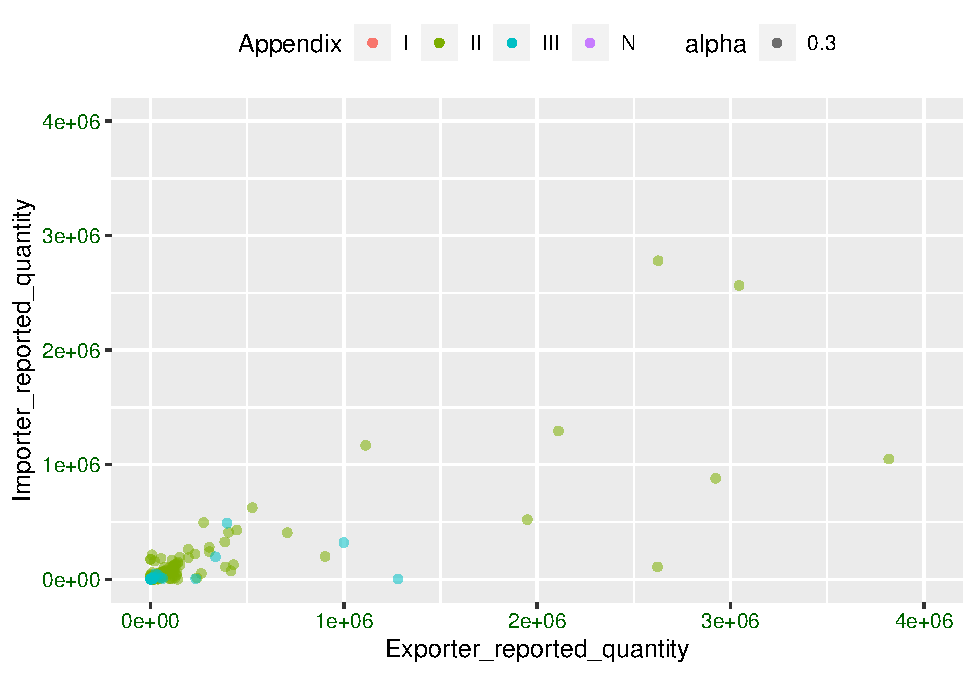
\includegraphics{Wood_ENV872_Project_files/figure-latex/unnamed-chunk-4-1.pdf}

\begin{Shaded}
\begin{Highlighting}[]
\NormalTok{Import.distribution }\OtherTok{\textless{}{-}} \FunctionTok{ggplot}\NormalTok{(CITESPoaching2016, }\FunctionTok{aes}\NormalTok{(}\AttributeTok{x =}\NormalTok{ Importer\_reported\_quantity)) }\SpecialCharTok{+}
    \FunctionTok{geom\_histogram}\NormalTok{(}\AttributeTok{binwidth =} \DecValTok{50}\NormalTok{, }\AttributeTok{colour =} \StringTok{"dark green"}\NormalTok{, }\AttributeTok{fill =} \StringTok{"light green"}\NormalTok{, }\AttributeTok{alpha =} \FloatTok{0.3}\NormalTok{) }\SpecialCharTok{+}
    \FunctionTok{xlim}\NormalTok{(}\DecValTok{0}\NormalTok{, }\DecValTok{1500}\NormalTok{) }\SpecialCharTok{+} \FunctionTok{ylim}\NormalTok{(}\DecValTok{0}\NormalTok{, }\DecValTok{2500}\NormalTok{) }\SpecialCharTok{+} \FunctionTok{labs}\NormalTok{(}\AttributeTok{title =} \StringTok{"Import Distribution"}\NormalTok{)}
\FunctionTok{print}\NormalTok{(Import.distribution)}
\end{Highlighting}
\end{Shaded}

\begin{verbatim}
## Warning: Removed 37201 rows containing non-finite values (stat_bin).
## Removed 3 rows containing missing values (geom_bar).
\end{verbatim}

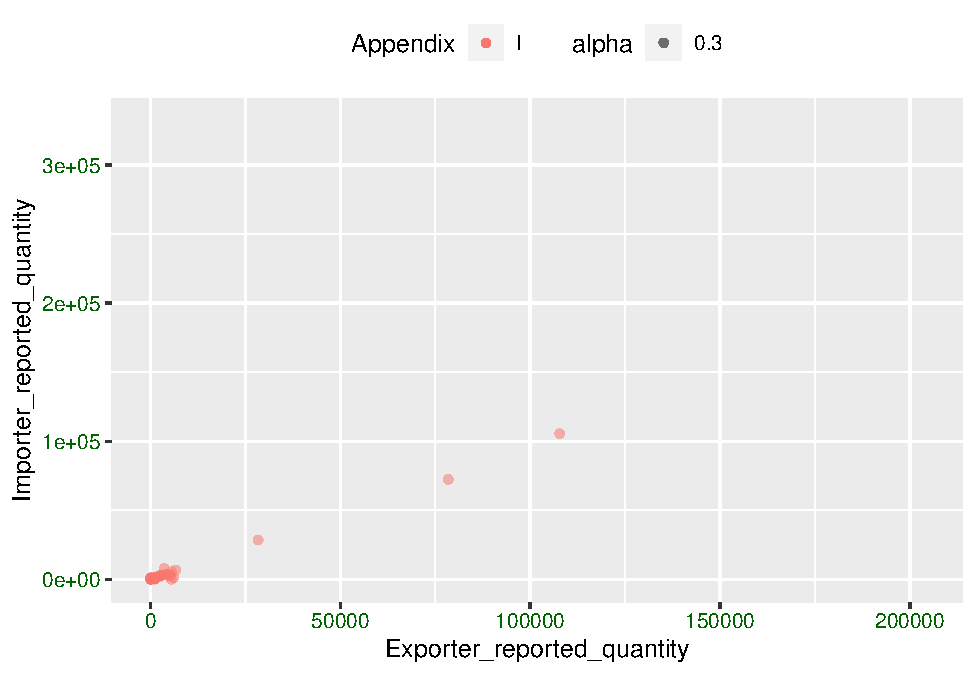
\includegraphics{Wood_ENV872_Project_files/figure-latex/unnamed-chunk-4-2.pdf}

\begin{Shaded}
\begin{Highlighting}[]
\NormalTok{Graphnew }\OtherTok{\textless{}{-}} \FunctionTok{ggplot}\NormalTok{(CITESPoaching2016, }\FunctionTok{aes}\NormalTok{(}\AttributeTok{x =}\NormalTok{ Exporter\_reported\_quantity, }\AttributeTok{y =}\NormalTok{ Importer\_reported\_quantity,}
    \AttributeTok{color =}\NormalTok{ Appendix, }\AttributeTok{alpha =} \FloatTok{0.3}\NormalTok{)) }\SpecialCharTok{+} \FunctionTok{geom\_point}\NormalTok{() }\SpecialCharTok{+} \FunctionTok{xlim}\NormalTok{(}\DecValTok{0}\NormalTok{, }\FloatTok{4e+06}\NormalTok{) }\SpecialCharTok{+} \FunctionTok{ylim}\NormalTok{(}\DecValTok{0}\NormalTok{, }\FloatTok{4e+06}\NormalTok{)}

\FunctionTok{print}\NormalTok{(Graphnew)}
\end{Highlighting}
\end{Shaded}

\begin{verbatim}
## Warning: Removed 58437 rows containing missing values (geom_point).
\end{verbatim}

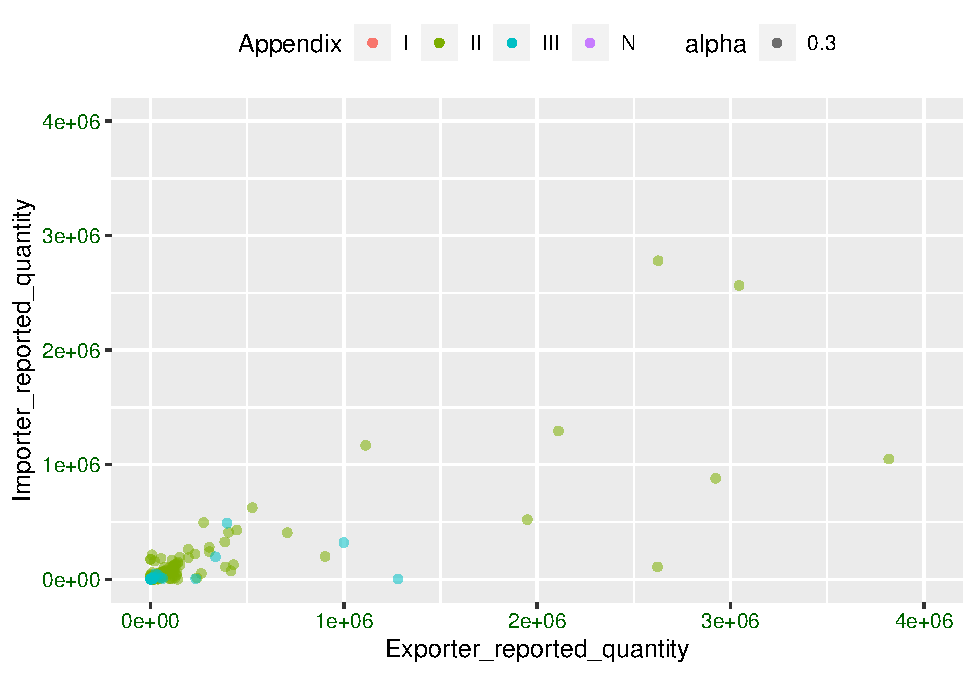
\includegraphics{Wood_ENV872_Project_files/figure-latex/unnamed-chunk-4-3.pdf}

\begin{Shaded}
\begin{Highlighting}[]
\NormalTok{Appendix1 }\OtherTok{\textless{}{-}} \FunctionTok{ggplot}\NormalTok{(}\FunctionTok{subset}\NormalTok{(CITESPoaching2016, Appendix }\SpecialCharTok{==} \StringTok{"I"}\NormalTok{), }\FunctionTok{aes}\NormalTok{(}\AttributeTok{x =}\NormalTok{ Exporter\_reported\_quantity,}
    \AttributeTok{y =}\NormalTok{ Importer\_reported\_quantity, }\AttributeTok{color =}\NormalTok{ Appendix, }\AttributeTok{alpha =} \FloatTok{0.3}\NormalTok{)) }\SpecialCharTok{+} \FunctionTok{geom\_point}\NormalTok{()}
\FunctionTok{print}\NormalTok{(Appendix1)}
\end{Highlighting}
\end{Shaded}

\begin{verbatim}
## Warning: Removed 5059 rows containing missing values (geom_point).
\end{verbatim}

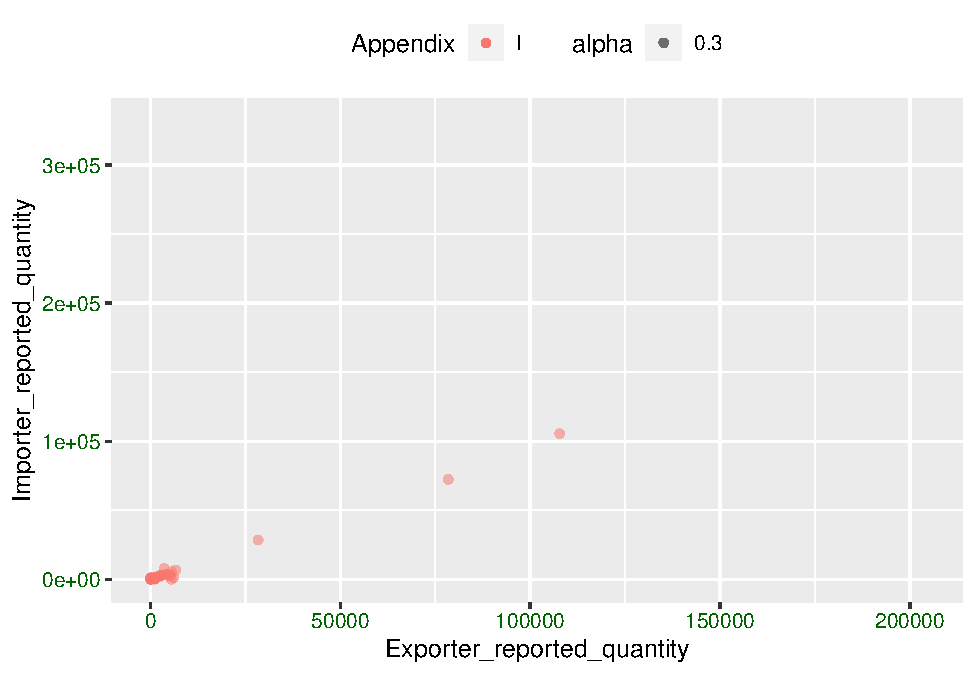
\includegraphics{Wood_ENV872_Project_files/figure-latex/unnamed-chunk-4-4.pdf}

\begin{Shaded}
\begin{Highlighting}[]
\CommentTok{\# Remove Null Values and combine Export and Import amounts into a total}
\CommentTok{\# reported quantity column. Previous graphs should not contain the zeros.}

\NormalTok{CITESPoaching2016[}\StringTok{"Importer\_reported\_quantity"}\NormalTok{][}\FunctionTok{is.na}\NormalTok{(CITESPoaching2016[}\StringTok{"Importer\_reported\_quantity"}\NormalTok{])] }\OtherTok{\textless{}{-}} \DecValTok{0}

\NormalTok{CITESPoaching2016[}\StringTok{"Exporter\_reported\_quantity"}\NormalTok{][}\FunctionTok{is.na}\NormalTok{(CITESPoaching2016[}\StringTok{"Exporter\_reported\_quantity"}\NormalTok{])] }\OtherTok{\textless{}{-}} \DecValTok{0}


\CommentTok{\# Visualizing countries with greater number of exports and imports Found}
\CommentTok{\# journal to visualize countries}
\CommentTok{\# https://journal.r{-}project.org/archive/2011{-}1/RJournal\_2011{-}1\_South.pdf}
\CommentTok{\# install.packages(\textquotesingle{}rworldmap\textquotesingle{})}
\FunctionTok{library}\NormalTok{(rworldmap)}

\CommentTok{\# Importer Countries}
\NormalTok{CITES\_Importer\_withmap }\OtherTok{\textless{}{-}} \FunctionTok{joinCountryData2Map}\NormalTok{(CITES2016\_Processed, }\AttributeTok{joinCode =} \StringTok{"ISO\_A2"}\NormalTok{,}
    \AttributeTok{nameJoinColumn =} \StringTok{"Importer"}\NormalTok{)}
\end{Highlighting}
\end{Shaded}

\begin{verbatim}
## 59647 codes from your data successfully matched countries in the map
## 1112 codes from your data failed to match with a country code in the map
## 41 codes from the map weren't represented in your data
\end{verbatim}

\begin{Shaded}
\begin{Highlighting}[]
\FunctionTok{mapDevice}\NormalTok{()  }\CommentTok{\#create world map shaped window}
\FunctionTok{mapCountryData}\NormalTok{(CITES\_Importer\_withmap, }\AttributeTok{nameColumnToPlot =} \StringTok{"Importer"}\NormalTok{)}
\end{Highlighting}
\end{Shaded}

\begin{verbatim}
## using catMethod='categorical' for non numeric data in mapCountryData
\end{verbatim}

\begin{Shaded}
\begin{Highlighting}[]
\NormalTok{Importerplot1 }\OtherTok{\textless{}{-}} \FunctionTok{ggplot}\NormalTok{(CITES2016\_Processed, }\FunctionTok{aes}\NormalTok{(}\AttributeTok{x =}\NormalTok{ Importer)) }\SpecialCharTok{+} \FunctionTok{geom\_bar}\NormalTok{(}\AttributeTok{binwidth =} \DecValTok{50}\NormalTok{,}
    \AttributeTok{colour =} \StringTok{"blue"}\NormalTok{, }\AttributeTok{fill =} \StringTok{"light blue"}\NormalTok{, }\AttributeTok{alpha =} \FloatTok{0.3}\NormalTok{)}
\end{Highlighting}
\end{Shaded}

\begin{verbatim}
## Warning: Ignoring unknown parameters: binwidth
\end{verbatim}

\begin{Shaded}
\begin{Highlighting}[]
\FunctionTok{print}\NormalTok{(Importerplot1)}

\CommentTok{\# Difficult to interpret. Wrangle new dataset and create bar graph with only}
\CommentTok{\# top 10 import countries:}

\FunctionTok{table}\NormalTok{(CITES2016\_Processed}\SpecialCharTok{$}\NormalTok{Importer)}
\end{Highlighting}
\end{Shaded}

\begin{verbatim}
## 
##   AD   AE   AF   AG   AI   AL   AM   AN   AO   AR   AT   AU   AW   AZ   BA   BB 
##   29 1295   94   14    1   95  103   12   60  286  498  490   99  168  145  116 
##   BD   BE   BF   BG   BH   BJ   BL   BM   BN   BO   BQ   BR   BS   BW   BY   BZ 
##  153  390    1   94  378    2   58   12   83    4   42  381   48    4  297    3 
##   CA   CC   CD   CF   CG   CH   CI   CL   CM   CN   CO   CR   CU   CV   CW   CY 
## 1230    4   21    1   17 2226   42  299    8 1779   74  108    7    7  107   87 
##   CZ   DE   DJ   DK   DM   DO   DZ   EC   EE   EG   ER   ES   ET   FI   FJ   FO 
##  409 4652    1  446    1   92   69   16   20  134    3  693   11   53    5   24 
##   FR   GA   GB   GD   GE   GF   GG   GH   GI   GL   GM   GN   GP   GQ   GR   GT 
## 2350    4 1121    4  145   60   17   51   45    9    1    2  127    2  138  197 
##   GU   GY   HK   HN   HR   HT   HU   ID   IE   IL   IM   IN   IQ   IR   IS   IT 
##   23    2 2249    8    9    5  124  337   88  362    6  317  202  252   29 1136 
##   JE   JM   JO   JP   KE   KG   KH   KN   KP   KR   KW   KY   KZ   LA   LB   LC 
##   29    9  220 4797   36   68   35   13  111 1206  671   21  376   30  385    5 
##   LI   LK   LR   LT   LU   LV   LY   MA   MC   MD   ME   MF   MG   MK   ML   MM 
##   10   22    2   48   12   29   25  176  172  159   92   18   93  142    3   28 
##   MN   MO   MP   MQ   MR   MT   MU   MV   MW   MX   MY   MZ   NC   NE   NG   NI 
##   18  265    8  114    2    4   86   97    8  608  622   12    9    4   87   11 
##   NL   NO   NP   NZ   OM   PA   PE   PF   PG   PH   PK   PL   PR   PT   PW   PY 
##  675  884   68  489  332  117  117    5    3  378  260  251    9  148    6   22 
##   QA   RE   RO   RS   RU   RW   SA   SC   SD   SE   SG   SI   SK   SM   SN   SR 
##  781  147   84  141  861    3  407    1   14  213 1364   24   68  122   87   99 
##   SU   SV   SX   SY   SZ   TC   TD   TF   TG   TH   TJ   TK   TL   TM   TN   TR 
##    7   22   64    4    7    1    2    2    5  812   26    2    2   63   98  938 
##   TT   TW   TZ   UA   UG   US   UY   UZ   VC   VE   VG   VI   VN   WS   XV   XX 
##   61 1066   13  483   19 8678   23  163    2   28   14    2  231    1   39  499 
##   YE   YT   YU   ZA   ZM   ZW 
##    2    1    5  523    8   74
\end{verbatim}

\begin{Shaded}
\begin{Highlighting}[]
\NormalTok{ImporterData }\OtherTok{\textless{}{-}}\NormalTok{ CITES2016\_Processed }\SpecialCharTok{\%\textgreater{}\%}
    \FunctionTok{group\_by}\NormalTok{(Importer) }\SpecialCharTok{\%\textgreater{}\%}
    \FunctionTok{summarise}\NormalTok{(Importer, }\AttributeTok{count =} \FunctionTok{n}\NormalTok{()) }\SpecialCharTok{\%\textgreater{}\%}
    \FunctionTok{filter}\NormalTok{(Importer }\SpecialCharTok{==} \StringTok{"US"} \SpecialCharTok{|}\NormalTok{ Importer }\SpecialCharTok{==} \StringTok{"JP"} \SpecialCharTok{|}\NormalTok{ Importer }\SpecialCharTok{==} \StringTok{"DE"} \SpecialCharTok{|}\NormalTok{ Importer }\SpecialCharTok{==} \StringTok{"FR"} \SpecialCharTok{|}
\NormalTok{        Importer }\SpecialCharTok{==} \StringTok{"HK"} \SpecialCharTok{|}\NormalTok{ Importer }\SpecialCharTok{==} \StringTok{"CH"} \SpecialCharTok{|}\NormalTok{ Importer }\SpecialCharTok{==} \StringTok{"CN"} \SpecialCharTok{|}\NormalTok{ Importer }\SpecialCharTok{==} \StringTok{"SG"} \SpecialCharTok{|}
\NormalTok{        Importer }\SpecialCharTok{==} \StringTok{"AE"} \SpecialCharTok{|}\NormalTok{ Importer }\SpecialCharTok{==} \StringTok{"CA"}\NormalTok{)}
\end{Highlighting}
\end{Shaded}

\begin{verbatim}
## `summarise()` has grouped output by 'Importer'. You can override using the
## `.groups` argument.
\end{verbatim}

\begin{Shaded}
\begin{Highlighting}[]
\NormalTok{Importerplot2 }\OtherTok{\textless{}{-}} \FunctionTok{ggplot}\NormalTok{(ImporterData, }\FunctionTok{aes}\NormalTok{(}\AttributeTok{x =}\NormalTok{ Importer)) }\SpecialCharTok{+} \FunctionTok{geom\_bar}\NormalTok{(}\AttributeTok{binwidth =} \DecValTok{50}\NormalTok{,}
    \AttributeTok{colour =} \StringTok{"purple"}\NormalTok{, }\AttributeTok{fill =} \StringTok{"lavender"}\NormalTok{, }\AttributeTok{alpha =} \FloatTok{0.3}\NormalTok{)}
\end{Highlighting}
\end{Shaded}

\begin{verbatim}
## Warning: Ignoring unknown parameters: binwidth
\end{verbatim}

\begin{Shaded}
\begin{Highlighting}[]
\FunctionTok{print}\NormalTok{(Importerplot2)}

\CommentTok{\# Exporter Countries}
\NormalTok{CITES\_Exporter\_withmap }\OtherTok{\textless{}{-}} \FunctionTok{joinCountryData2Map}\NormalTok{(CITES2016\_Processed, }\AttributeTok{joinCode =} \StringTok{"ISO\_A2"}\NormalTok{,}
    \AttributeTok{nameJoinColumn =} \StringTok{"Exporter"}\NormalTok{)}
\end{Highlighting}
\end{Shaded}

\begin{verbatim}
## 60130 codes from your data successfully matched countries in the map
## 629 codes from your data failed to match with a country code in the map
## 44 codes from the map weren't represented in your data
\end{verbatim}

\begin{Shaded}
\begin{Highlighting}[]
\FunctionTok{mapDevice}\NormalTok{()  }\CommentTok{\#create world map shaped window}
\FunctionTok{mapCountryData}\NormalTok{(CITES\_Exporter\_withmap, }\AttributeTok{nameColumnToPlot =} \StringTok{"Exporter"}\NormalTok{)}
\end{Highlighting}
\end{Shaded}

\begin{verbatim}
## using catMethod='categorical' for non numeric data in mapCountryData
\end{verbatim}

\begin{Shaded}
\begin{Highlighting}[]
\NormalTok{Exporterplot1 }\OtherTok{\textless{}{-}} \FunctionTok{ggplot}\NormalTok{(CITES2016\_Processed, }\FunctionTok{aes}\NormalTok{(}\AttributeTok{x =}\NormalTok{ Exporter)) }\SpecialCharTok{+} \FunctionTok{geom\_bar}\NormalTok{(}\AttributeTok{binwidth =} \DecValTok{50}\NormalTok{,}
    \AttributeTok{colour =} \StringTok{"blue"}\NormalTok{, }\AttributeTok{fill =} \StringTok{"light blue"}\NormalTok{, }\AttributeTok{alpha =} \FloatTok{0.3}\NormalTok{)}
\end{Highlighting}
\end{Shaded}

\begin{verbatim}
## Warning: Ignoring unknown parameters: binwidth
\end{verbatim}

\begin{Shaded}
\begin{Highlighting}[]
\FunctionTok{print}\NormalTok{(Exporterplot1)}

\CommentTok{\# Difficult to interpret. Wrangle new dataset and create bar graph with only}
\CommentTok{\# top 10 export countries:}

\FunctionTok{table}\NormalTok{(CITES2016\_Processed}\SpecialCharTok{$}\NormalTok{Exporter)}
\end{Highlighting}
\end{Shaded}

\begin{verbatim}
## 
##   AD   AE   AG   AL   AM   AO   AQ   AR   AT   AU   AW   AZ   BB   BD   BE   BG 
##    2  838    8    5   27   10    2  302  305 1391    2   10   35    2 1153   15 
##   BH   BI   BJ   BL   BM   BO   BR   BS   BW   BY   BZ   CA   CD   CF   CG   CH 
##   52    1   24    4   35   16  463   42    3   30   15 1040   46    9   17 1339 
##   CI   CK   CL   CM   CN   CO   CR   CU   CV   CW   CY   CZ   DD   DE   DK   DM 
##   22   15   46   35 1133  497   52   86    1   27    1  751    1 1859  313    7 
##   DO   EC   EE   EG   ER   ES   ET   FI   FJ   FK   FM   FO   FR   GA   GB   GD 
##  109 1500   35    8    2 1056   73   35  501    9   52    1 2720   11 1038    5 
##   GE   GG   GH   GI   GL   GM   GN   GP   GQ   GR   GS   GT   GW   GY   HK   HN 
##   19   18   57    2  109    1    4    1   11   84    2   21    7  314  730    6 
##   HR   HT   HU   ID   IE   IL   IM   IN   IO   IQ   IR   IS   IT   JE   JM   JO 
##   16   10   49 6449   33   36    1  345   10    4    3   15 4776   82   69   14 
##   JP   KE   KG   KH   KI   KM   KN   KR   KW   KY   KZ   LA   LB   LC   LI   LK 
##  838  114   26   35    2    2   12  273  283   17   77  142   40    4    2   87 
##   LR   LS   LT   LU   LV   MA   MC   MG   MH   MK   ML   MM   MN   MO   MT   MU 
##   11    1   24   64   39   38  421  867   56   28   60   16   51   52   37   39 
##   MV   MW   MX   MY   MZ   NC   NE   NG   NI   NL   NO   NP   NZ   OM   PA   PE 
##    6   15  378 1258   80    2    1   15   60 7156   97    7   97  115  113 1226 
##   PF   PG   PH   PK   PL   PT   PW   PY   QA   RO   RS   RU   RW   SA   SB   SC 
##    8   22 1150   37   35  179   64   12  172   27   66  194    5   35   95   29 
##   SD   SE   SG   SH   SI   SK   SL   SM   SN   SR   ST   SV   SX   SY   SZ   TC 
##   37  101 1315    5   45   35    1   19   28  117    6   65    8   10    1    9 
##   TD   TG   TH   TJ   TK   TL   TN   TO   TR   TT   TW   TZ   UA   UG   US   UY 
##    3   65 1371   15    1    1   36  275  218   14  618  164   93   56 3879   49 
##   UZ   VC   VE   VG   VN   VU   XV   XX   YE   ZA   ZM   ZW   ZZ 
##  110    1   74   15  189    4    3   61    5 1369  128  524    6
\end{verbatim}

\begin{Shaded}
\begin{Highlighting}[]
\NormalTok{ExporterData }\OtherTok{\textless{}{-}}\NormalTok{ CITES2016\_Processed }\SpecialCharTok{\%\textgreater{}\%}
    \FunctionTok{group\_by}\NormalTok{(Exporter) }\SpecialCharTok{\%\textgreater{}\%}
    \FunctionTok{summarise}\NormalTok{(Exporter, }\AttributeTok{count =} \FunctionTok{n}\NormalTok{()) }\SpecialCharTok{\%\textgreater{}\%}
    \FunctionTok{filter}\NormalTok{(Exporter }\SpecialCharTok{==} \StringTok{"NL"} \SpecialCharTok{|}\NormalTok{ Exporter }\SpecialCharTok{==} \StringTok{"ID"} \SpecialCharTok{|}\NormalTok{ Exporter }\SpecialCharTok{==} \StringTok{"IT"} \SpecialCharTok{|}\NormalTok{ Exporter }\SpecialCharTok{==} \StringTok{"US"} \SpecialCharTok{|}
\NormalTok{        Exporter }\SpecialCharTok{==} \StringTok{"FR"} \SpecialCharTok{|}\NormalTok{ Exporter }\SpecialCharTok{==} \StringTok{"DE"} \SpecialCharTok{|}\NormalTok{ Exporter }\SpecialCharTok{==} \StringTok{"EC"} \SpecialCharTok{|}\NormalTok{ Exporter }\SpecialCharTok{==} \StringTok{"AU"} \SpecialCharTok{|}
\NormalTok{        Exporter }\SpecialCharTok{==} \StringTok{"TH"} \SpecialCharTok{|}\NormalTok{ Exporter }\SpecialCharTok{==} \StringTok{"ZA"}\NormalTok{)}
\end{Highlighting}
\end{Shaded}

\begin{verbatim}
## `summarise()` has grouped output by 'Exporter'. You can override using the
## `.groups` argument.
\end{verbatim}

\begin{Shaded}
\begin{Highlighting}[]
\NormalTok{Exporterplot2 }\OtherTok{\textless{}{-}} \FunctionTok{ggplot}\NormalTok{(ExporterData, }\FunctionTok{aes}\NormalTok{(}\AttributeTok{x =}\NormalTok{ Exporter)) }\SpecialCharTok{+} \FunctionTok{geom\_bar}\NormalTok{(}\AttributeTok{binwidth =} \DecValTok{50}\NormalTok{,}
    \AttributeTok{colour =} \StringTok{"blue"}\NormalTok{, }\AttributeTok{fill =} \StringTok{"light blue"}\NormalTok{, }\AttributeTok{alpha =} \FloatTok{0.3}\NormalTok{)}
\end{Highlighting}
\end{Shaded}

\begin{verbatim}
## Warning: Ignoring unknown parameters: binwidth
\end{verbatim}

\begin{Shaded}
\begin{Highlighting}[]
\FunctionTok{print}\NormalTok{(Exporterplot2)}

\CommentTok{\# Which Classes get poached most often?}

\NormalTok{Classplot1 }\OtherTok{\textless{}{-}} \FunctionTok{ggplot}\NormalTok{(CITES2016\_Processed, }\FunctionTok{aes}\NormalTok{(}\AttributeTok{x =}\NormalTok{ Class)) }\SpecialCharTok{+} \FunctionTok{geom\_bar}\NormalTok{(}\FunctionTok{aes}\NormalTok{(}\AttributeTok{fill =}\NormalTok{ Class)) }\SpecialCharTok{+}
    \FunctionTok{labs}\NormalTok{(}\AttributeTok{title =} \StringTok{"Classes of poaching occurances 2016"}\NormalTok{, }\AttributeTok{x =} \StringTok{"Class"}\NormalTok{, }\AttributeTok{y =} \StringTok{"Count"}\NormalTok{) }\SpecialCharTok{+}
    \FunctionTok{theme}\NormalTok{(}\AttributeTok{legend.position =} \StringTok{"none"}\NormalTok{) }\SpecialCharTok{+} \FunctionTok{coord\_flip}\NormalTok{()}

\FunctionTok{print}\NormalTok{(Classplot1)}


\CommentTok{\# This has a lot of NAs perhaps they didn\textquotesingle{}t record always the Class Faceted by}
\CommentTok{\# appendix}

\NormalTok{Classplot2 }\OtherTok{\textless{}{-}} \FunctionTok{ggplot}\NormalTok{(CITES2016\_Processed, }\FunctionTok{aes}\NormalTok{(}\AttributeTok{x =}\NormalTok{ Class)) }\SpecialCharTok{+} \FunctionTok{geom\_bar}\NormalTok{(}\FunctionTok{aes}\NormalTok{(}\AttributeTok{fill =}\NormalTok{ Class)) }\SpecialCharTok{+}
    \FunctionTok{labs}\NormalTok{(}\AttributeTok{title =} \StringTok{"Classes of poaching occurances 2016"}\NormalTok{, }\AttributeTok{x =} \StringTok{"Class"}\NormalTok{, }\AttributeTok{y =} \StringTok{"Count"}\NormalTok{) }\SpecialCharTok{+}
    \FunctionTok{coord\_flip}\NormalTok{() }\SpecialCharTok{+} \FunctionTok{facet\_grid}\NormalTok{(}\AttributeTok{rows =} \StringTok{"Appendix"}\NormalTok{) }\SpecialCharTok{+} \FunctionTok{theme}\NormalTok{(}\AttributeTok{axis.text =} \FunctionTok{element\_text}\NormalTok{(}\AttributeTok{size =} \DecValTok{5}\NormalTok{))}
\FunctionTok{print}\NormalTok{(Classplot2)}

\CommentTok{\# create a facet dataset for Appendix I}

\NormalTok{AppendixI\_Facet }\OtherTok{\textless{}{-}}\NormalTok{ CITES2016\_Processed }\SpecialCharTok{\%\textgreater{}\%}
    \FunctionTok{filter}\NormalTok{(Appendix }\SpecialCharTok{==} \StringTok{"I"}\NormalTok{)}


\CommentTok{\# A closer look at Mammalia}

\NormalTok{Mammalia\_terms }\OtherTok{\textless{}{-}} \FunctionTok{ggplot}\NormalTok{(}\FunctionTok{subset}\NormalTok{(AppendixI\_Facet, Class }\SpecialCharTok{\%in\%} \StringTok{"Mammalia"}\NormalTok{), }\FunctionTok{aes}\NormalTok{(}\AttributeTok{x =}\NormalTok{ Term)) }\SpecialCharTok{+}
    \FunctionTok{geom\_bar}\NormalTok{(}\FunctionTok{aes}\NormalTok{(}\AttributeTok{fill =}\NormalTok{ Term)) }\SpecialCharTok{+} \FunctionTok{coord\_flip}\NormalTok{() }\SpecialCharTok{+} \FunctionTok{theme}\NormalTok{(}\AttributeTok{axis.text =} \FunctionTok{element\_text}\NormalTok{(}\AttributeTok{size =} \DecValTok{5}\NormalTok{),}
    \AttributeTok{legend.key.size =} \FunctionTok{unit}\NormalTok{(}\FloatTok{0.2}\NormalTok{, }\StringTok{"cm"}\NormalTok{), }\AttributeTok{legend.key.height =} \FunctionTok{unit}\NormalTok{(}\FloatTok{0.2}\NormalTok{, }\StringTok{"cm"}\NormalTok{), }\AttributeTok{legend.key.width =} \FunctionTok{unit}\NormalTok{(}\FloatTok{0.2}\NormalTok{,}
        \StringTok{"cm"}\NormalTok{), }\AttributeTok{legend.title =} \FunctionTok{element\_text}\NormalTok{(}\AttributeTok{size =} \DecValTok{3}\NormalTok{), }\AttributeTok{legend.text =} \FunctionTok{element\_text}\NormalTok{(}\AttributeTok{size =} \DecValTok{3}\NormalTok{))}

\FunctionTok{print}\NormalTok{(Mammalia\_terms)}

\CommentTok{\# A closer look at Aves}

\NormalTok{Aves\_terms }\OtherTok{\textless{}{-}} \FunctionTok{ggplot}\NormalTok{(}\FunctionTok{subset}\NormalTok{(AppendixI\_Facet, Class }\SpecialCharTok{\%in\%} \StringTok{"Aves"}\NormalTok{), }\FunctionTok{aes}\NormalTok{(}\AttributeTok{x =}\NormalTok{ Term)) }\SpecialCharTok{+}
    \FunctionTok{geom\_bar}\NormalTok{(}\FunctionTok{aes}\NormalTok{(}\AttributeTok{fill =}\NormalTok{ Term)) }\SpecialCharTok{+} \FunctionTok{coord\_flip}\NormalTok{() }\SpecialCharTok{+} \FunctionTok{theme}\NormalTok{(}\AttributeTok{axis.text =} \FunctionTok{element\_text}\NormalTok{(}\AttributeTok{size =} \DecValTok{5}\NormalTok{),}
    \AttributeTok{legend.key.size =} \FunctionTok{unit}\NormalTok{(}\FloatTok{0.2}\NormalTok{, }\StringTok{"cm"}\NormalTok{), }\AttributeTok{legend.key.height =} \FunctionTok{unit}\NormalTok{(}\FloatTok{0.2}\NormalTok{, }\StringTok{"cm"}\NormalTok{), }\AttributeTok{legend.key.width =} \FunctionTok{unit}\NormalTok{(}\FloatTok{0.2}\NormalTok{,}
        \StringTok{"cm"}\NormalTok{), }\AttributeTok{legend.title =} \FunctionTok{element\_text}\NormalTok{(}\AttributeTok{size =} \DecValTok{3}\NormalTok{), }\AttributeTok{legend.text =} \FunctionTok{element\_text}\NormalTok{(}\AttributeTok{size =} \DecValTok{3}\NormalTok{))}

\FunctionTok{print}\NormalTok{(Aves\_terms)}

\CommentTok{\# A closer look at Reptilia}

\NormalTok{Reptilia\_terms }\OtherTok{\textless{}{-}} \FunctionTok{ggplot}\NormalTok{(}\FunctionTok{subset}\NormalTok{(AppendixI\_Facet, Class }\SpecialCharTok{\%in\%} \StringTok{"Reptilia"}\NormalTok{), }\FunctionTok{aes}\NormalTok{(}\AttributeTok{x =}\NormalTok{ Term)) }\SpecialCharTok{+}
    \FunctionTok{geom\_bar}\NormalTok{(}\FunctionTok{aes}\NormalTok{(}\AttributeTok{fill =}\NormalTok{ Term)) }\SpecialCharTok{+} \FunctionTok{coord\_flip}\NormalTok{() }\SpecialCharTok{+} \FunctionTok{theme}\NormalTok{(}\AttributeTok{axis.text =} \FunctionTok{element\_text}\NormalTok{(}\AttributeTok{size =} \DecValTok{5}\NormalTok{),}
    \AttributeTok{legend.key.size =} \FunctionTok{unit}\NormalTok{(}\FloatTok{0.2}\NormalTok{, }\StringTok{"cm"}\NormalTok{), }\AttributeTok{legend.key.height =} \FunctionTok{unit}\NormalTok{(}\FloatTok{0.2}\NormalTok{, }\StringTok{"cm"}\NormalTok{), }\AttributeTok{legend.key.width =} \FunctionTok{unit}\NormalTok{(}\FloatTok{0.2}\NormalTok{,}
        \StringTok{"cm"}\NormalTok{), }\AttributeTok{legend.title =} \FunctionTok{element\_text}\NormalTok{(}\AttributeTok{size =} \DecValTok{3}\NormalTok{), }\AttributeTok{legend.text =} \FunctionTok{element\_text}\NormalTok{(}\AttributeTok{size =} \DecValTok{3}\NormalTok{))}

\FunctionTok{print}\NormalTok{(Reptilia\_terms)}

\CommentTok{\# Why arent plants represented in Class? monocotyledons or dicotyledons not}
\CommentTok{\# depicted so potentiall in NAs}

\NormalTok{AppendixI\_Facet[}\StringTok{"Class"}\NormalTok{][}\FunctionTok{is.na}\NormalTok{(AppendixI\_Facet[}\StringTok{"Class"}\NormalTok{])] }\OtherTok{\textless{}{-}} \StringTok{"Not\_recorded"}

\NormalTok{NA\_terms }\OtherTok{\textless{}{-}} \FunctionTok{ggplot}\NormalTok{(}\FunctionTok{subset}\NormalTok{(AppendixI\_Facet, Class }\SpecialCharTok{\%in\%} \StringTok{"Not\_recorded"}\NormalTok{), }\FunctionTok{aes}\NormalTok{(}\AttributeTok{x =}\NormalTok{ Term)) }\SpecialCharTok{+}
    \FunctionTok{geom\_bar}\NormalTok{(}\FunctionTok{aes}\NormalTok{(}\AttributeTok{fill =}\NormalTok{ Term)) }\SpecialCharTok{+} \FunctionTok{coord\_flip}\NormalTok{() }\SpecialCharTok{+} \FunctionTok{theme}\NormalTok{(}\AttributeTok{axis.text =} \FunctionTok{element\_text}\NormalTok{(}\AttributeTok{size =} \DecValTok{5}\NormalTok{),}
    \AttributeTok{legend.key.size =} \FunctionTok{unit}\NormalTok{(}\FloatTok{0.2}\NormalTok{, }\StringTok{"cm"}\NormalTok{), }\AttributeTok{legend.key.height =} \FunctionTok{unit}\NormalTok{(}\FloatTok{0.2}\NormalTok{, }\StringTok{"cm"}\NormalTok{), }\AttributeTok{legend.key.width =} \FunctionTok{unit}\NormalTok{(}\FloatTok{0.2}\NormalTok{,}
        \StringTok{"cm"}\NormalTok{), }\AttributeTok{legend.title =} \FunctionTok{element\_text}\NormalTok{(}\AttributeTok{size =} \DecValTok{3}\NormalTok{), }\AttributeTok{legend.text =} \FunctionTok{element\_text}\NormalTok{(}\AttributeTok{size =} \DecValTok{3}\NormalTok{))}

\FunctionTok{print}\NormalTok{(NA\_terms)}
\end{Highlighting}
\end{Shaded}

\hypertarget{rationale-and-research-questions}{%
\section{Rationale and Research
Questions}\label{rationale-and-research-questions}}

Does level of protection, class, term affect the amount
exported/imported?

What might the best set of predictors for Poaching?

\begin{Shaded}
\begin{Highlighting}[]
\CommentTok{\# Two way ANOVA}


\CommentTok{\# Linear modeling}

\CommentTok{\# 1.How Does Reported Poaching Quantity vary over Class and Term for only}
\CommentTok{\# Appendix 1.}

\NormalTok{Poaching}\FloatTok{.2}\NormalTok{way }\OtherTok{\textless{}{-}} \FunctionTok{aov}\NormalTok{(}\AttributeTok{data =}\NormalTok{ AppendixI\_Facet, Reported\_quantity }\SpecialCharTok{\textasciitilde{}}\NormalTok{ Class }\SpecialCharTok{+}\NormalTok{ Term)}
\FunctionTok{summary}\NormalTok{(Poaching}\FloatTok{.2}\NormalTok{way)}
\end{Highlighting}
\end{Shaded}

\begin{verbatim}
##              Df    Sum Sq   Mean Sq F value   Pr(>F)    
## Class         6 4.467e+09 744583316   9.911 1.37e-10 ***
## Term         26 3.259e+09 125332949   1.668   0.0198 *  
## Residuals   853 6.408e+10  75125682                     
## ---
## Signif. codes:  0 '***' 0.001 '**' 0.01 '*' 0.05 '.' 0.1 ' ' 1
## 4768 observations deleted due to missingness
\end{verbatim}

\begin{Shaded}
\begin{Highlighting}[]
\CommentTok{\# P{-}value is small. Reject our null hypothesis that the mean across our groups}
\CommentTok{\# is different.  Not enough information to tell us which groups are differing}

\NormalTok{Poaching}\FloatTok{.2}\NormalTok{way2lm }\OtherTok{\textless{}{-}} \FunctionTok{lm}\NormalTok{(}\AttributeTok{data =}\NormalTok{ AppendixI\_Facet, Reported\_quantity }\SpecialCharTok{\textasciitilde{}}\NormalTok{ Class }\SpecialCharTok{+}\NormalTok{ Term)}
\FunctionTok{summary}\NormalTok{(Poaching}\FloatTok{.2}\NormalTok{way2lm)}
\end{Highlighting}
\end{Shaded}

\begin{verbatim}
## 
## Call:
## lm(formula = Reported_quantity ~ Class + Term, data = AppendixI_Facet)
## 
## Residuals:
##    Min     1Q Median     3Q    Max 
## -11288    -54    -40    -11 201942 
## 
## Coefficients:
##                                Estimate Std. Error t value Pr(>|t|)    
## (Intercept)                   1.128e+04  6.391e+03   1.764    0.078 .  
## ClassAmphibia                -1.169e+04  9.028e+03  -1.295    0.196    
## ClassAves                    -1.123e+04  1.542e+03  -7.282 7.46e-13 ***
## ClassCoelacanthi             -1.124e+04  9.390e+03  -1.197    0.232    
## ClassMammalia                -1.127e+04  1.812e+03  -6.220 7.76e-10 ***
## ClassNot_recorded            -1.123e+04  1.521e+03  -7.386 3.59e-13 ***
## ClassReptilia                -1.087e+04  2.602e+03  -4.175 3.28e-05 ***
## Termbodies                   -3.633e+01  7.032e+03  -0.005    0.996    
## Termbones                     2.100e+01  1.062e+04   0.002    0.998    
## Termcarvings                 -2.632e+02  6.612e+03  -0.040    0.968    
## Termcloth                     2.000e+00  1.062e+04   0.000    1.000    
## Termcosmetics                 5.633e+04  1.083e+04   5.204 2.45e-07 ***
## Termeggs                      7.105e+01  7.359e+03   0.010    0.992    
## Termfeathers                 -3.855e+01  1.069e+04  -0.004    0.997    
## Termfeet                     -2.000e+00  8.668e+03   0.000    1.000    
## Termgarments                 -2.610e+02  7.397e+03  -0.035    0.972    
## Termhair                      2.260e+02  1.062e+04   0.021    0.983    
## Termhorn carvings            -2.000e+00  1.062e+04   0.000    1.000    
## Termivory carvings            2.679e+01  6.248e+03   0.004    0.997    
## Termivory pieces              1.570e-11  1.062e+04   0.000    1.000    
## Termleather products (large) -4.078e+02  1.083e+04  -0.038    0.970    
## Termleather products (small) -3.057e+02  6.644e+03  -0.046    0.963    
## Termlive                      1.360e+01  6.230e+03   0.002    0.998    
## Termoil                       1.063e+04  1.083e+04   0.982    0.326    
## Termpiano keys                2.540e+02  7.912e+03   0.032    0.974    
## Termskin pieces               1.765e+03  1.083e+04   0.163    0.871    
## Termskins                     3.111e+02  6.609e+03   0.047    0.962    
## Termskulls                    5.000e+00  8.668e+03   0.001    1.000    
## Termspecimens                 4.168e+02  6.420e+03   0.065    0.948    
## Termteeth                     1.880e+02  8.668e+03   0.022    0.983    
## Termtrophies                  8.776e+00  6.253e+03   0.001    0.999    
## Termtusks                     1.830e+01  6.292e+03   0.003    0.998    
## Termwood product             -1.015e+01  6.776e+03  -0.001    0.999    
## ---
## Signif. codes:  0 '***' 0.001 '**' 0.01 '*' 0.05 '.' 0.1 ' ' 1
## 
## Residual standard error: 8668 on 853 degrees of freedom
##   (4768 observations deleted due to missingness)
## Multiple R-squared:  0.1076, Adjusted R-squared:  0.07412 
## F-statistic: 3.214 on 32 and 853 DF,  p-value: 9.76e-09
\end{verbatim}

\begin{Shaded}
\begin{Highlighting}[]
\CommentTok{\# means are different. Reject null}

\FunctionTok{TukeyHSD}\NormalTok{(Poaching}\FloatTok{.2}\NormalTok{way)}
\end{Highlighting}
\end{Shaded}

\begin{verbatim}
##   Tukey multiple comparisons of means
##     95% family-wise confidence level
## 
## Fit: aov(formula = Reported_quantity ~ Class + Term, data = AppendixI_Facet)
## 
## $Class
##                                   diff        lwr       upr     p adj
## Amphibia-Actinopteri     -1.128759e+04 -37247.303 14672.114 0.8588566
## Aves-Actinopteri         -1.123236e+04 -15772.442 -6692.282 0.0000000
## Coelacanthi-Actinopteri  -1.128759e+04 -37247.303 14672.114 0.8588566
## Mammalia-Actinopteri     -1.124305e+04 -15784.531 -6701.579 0.0000000
## Not_recorded-Actinopteri -1.123459e+04 -15717.307 -6751.882 0.0000000
## Reptilia-Actinopteri     -1.025311e+04 -15099.786 -5406.433 0.0000000
## Aves-Amphibia             5.523246e+01 -25616.737 25727.202 1.0000000
## Coelacanthi-Amphibia     -6.821210e-13 -36226.291 36226.291 1.0000000
## Mammalia-Amphibia         4.453965e+01 -25627.677 25716.756 1.0000000
## Not_recorded-Amphibia     5.300054e+01 -25608.886 25714.887 1.0000000
## Reptilia-Amphibia         1.034485e+03 -24693.476 26762.446 0.9999998
## Coelacanthi-Aves         -5.523246e+01 -25727.202 25616.737 1.0000000
## Mammalia-Aves            -1.069281e+01  -2412.478  2391.093 1.0000000
## Not_recorded-Aves        -2.231917e+00  -2290.961  2286.497 1.0000000
## Reptilia-Aves             9.792528e+02  -1959.087  3917.593 0.9572473
## Mammalia-Coelacanthi      4.453965e+01 -25627.677 25716.756 1.0000000
## Not_recorded-Coelacanthi  5.300054e+01 -25608.886 25714.887 1.0000000
## Reptilia-Coelacanthi      1.034485e+03 -24693.476 26762.446 0.9999998
## Not_recorded-Mammalia     8.460892e+00  -2283.036  2299.958 1.0000000
## Reptilia-Mammalia         9.899456e+02  -1950.551  3930.442 0.9551104
## Reptilia-Not_recorded     9.814847e+02  -1867.414  3830.384 0.9498794
## 
## $Term
##                                                            diff         lwr
## bodies-baleen                                     -4.077150e+00  -25419.651
## bones-baleen                                       2.100000e+01  -39352.637
## carvings-baleen                                   -6.595024e+02  -24558.394
## cloth-baleen                                       2.000000e+00  -39371.637
## cosmetics-baleen                                   5.574605e+04   16372.417
## eggs-baleen                                        1.009072e+02  -26796.408
## feathers-baleen                                   -8.692809e+00  -39382.330
## feet-baleen                                       -2.000000e+00  -32150.440
## garments-baleen                                   -5.995785e+02  -27496.893
## hair-baleen                                        2.260000e+02  -39147.637
## horn carvings-baleen                              -2.000000e+00  -39375.637
## ivory carvings-baleen                              2.679412e+01  -23147.033
## ivory pieces-baleen                                1.580247e-11  -39373.637
## leather products (large)-baleen                   -9.919456e+02  -40365.583
## leather products (small)-baleen                   -8.898534e+02  -24245.154
## live-baleen                                        3.723147e+01  -22734.787
## oil-baleen                                         1.004605e+04  -29327.583
## piano keys-baleen                                  2.540000e+02  -29093.376
## skin pieces-baleen                                 1.181054e+03  -38192.583
## skins-baleen                                      -2.587762e+02  -23539.003
## skulls-baleen                                      5.000000e+00  -32143.440
## specimens-baleen                                   1.327203e+02  -23345.181
## teeth-baleen                                       1.880000e+02  -31960.440
## trophies-baleen                                    8.775510e+00  -23182.891
## tusks-baleen                                       1.829730e+01  -23320.386
## wood product-baleen                                2.172093e+01  -24690.982
## bones-bodies                                       2.507715e+01  -34073.493
## carvings-bodies                                   -6.554252e+02  -14204.823
## cloth-bodies                                       6.077150e+00  -34092.493
## cosmetics-bodies                                   5.575013e+04   21651.561
## eggs-bodies                                        1.049843e+02  -18222.446
## feathers-bodies                                   -4.615658e+00  -34103.186
## feet-bodies                                        2.077150e+00  -25413.496
## garments-bodies                                   -5.955013e+02  -18922.932
## hair-bodies                                        2.300772e+02  -33868.493
## horn carvings-bodies                               2.077150e+00  -34096.493
## ivory carvings-bodies                              3.087127e+01  -12194.325
## ivory pieces-bodies                                4.077150e+00  -34094.493
## leather products (large)-bodies                   -9.878685e+02  -35086.439
## leather products (small)-bodies                   -8.857762e+02  -13451.572
## live-bodies                                        4.130862e+01  -11403.951
## oil-bodies                                         1.005013e+04  -24048.439
## piano keys-bodies                                  2.580772e+02  -21506.520
## skin pieces-bodies                                 1.185132e+03  -32913.439
## skins-bodies                                      -2.546991e+02  -12680.404
## skulls-bodies                                      9.077150e+00  -25406.496
## specimens-bodies                                   1.367974e+02  -12655.427
## teeth-bodies                                       1.920772e+02  -25223.496
## trophies-bodies                                    1.285266e+01  -12246.126
## tusks-bodies                                       2.237445e+01  -12512.509
## wood product-bodies                                2.579808e+01  -14912.302
## carvings-bones                                    -6.805024e+02  -33664.106
## cloth-bones                                       -1.900000e+01  -45483.760
## cosmetics-bones                                    5.572505e+04   10260.294
## eggs-bones                                         7.990719e+01  -35136.945
## feathers-bones                                    -2.969281e+01  -45494.453
## feet-bones                                        -2.300000e+01  -39396.637
## garments-bones                                    -6.205785e+02  -35837.430
## hair-bones                                         2.050000e+02  -45259.760
## horn carvings-bones                               -2.300000e+01  -45487.760
## ivory carvings-bones                               5.794118e+00  -32456.297
## ivory pieces-bones                                -2.100000e+01  -45485.760
## leather products (large)-bones                    -1.012946e+03  -46477.706
## leather products (small)-bones                    -9.108534e+02  -33502.741
## live-bones                                         1.623147e+01  -32160.249
## oil-bones                                          1.002505e+04  -35439.706
## piano keys-bones                                   2.330000e+02  -36888.821
## skin pieces-bones                                  1.160054e+03  -44304.706
## skins-bones                                       -2.797762e+02  -32817.909
## skulls-bones                                      -1.600000e+01  -39389.637
## specimens-bones                                    1.117203e+02  -32568.135
## teeth-bones                                        1.670000e+02  -39206.637
## trophies-bones                                    -1.222449e+01  -32487.053
## tusks-bones                                       -2.702703e+00  -32582.685
## wood product-bones                                 7.209262e-01  -33577.230
## cloth-carvings                                     6.615024e+02  -32322.101
## cosmetics-carvings                                 5.640556e+04   23421.953
## eggs-carvings                                      7.604095e+02  -15398.190
## feathers-carvings                                  6.508095e+02  -32332.794
## feet-carvings                                      6.575024e+02  -23241.389
## garments-carvings                                  5.992386e+01  -16098.676
## hair-carvings                                      8.855024e+02  -32098.101
## horn carvings-carvings                             6.575024e+02  -32326.101
## ivory carvings-carvings                            6.862965e+02   -7954.366
## ivory pieces-carvings                              6.595024e+02  -32324.101
## leather products (large)-carvings                 -3.324433e+02  -33316.047
## leather products (small)-carvings                 -2.303510e+02   -9346.537
## live-carvings                                      6.967338e+02   -6799.906
## oil-carvings                                       1.070556e+04  -22278.047
## piano keys-carvings                                9.135024e+02  -19059.061
## skin pieces-carvings                               1.840557e+03  -31143.047
## skins-carvings                                     4.007261e+02   -8521.368
## skulls-carvings                                    6.645024e+02  -23234.389
## specimens-carvings                                 7.922226e+02   -8633.627
## teeth-carvings                                     8.475024e+02  -23051.389
## trophies-carvings                                  6.682779e+02   -8020.116
## tusks-carvings                                     6.777997e+02   -8395.730
## wood product-carvings                              6.812233e+02  -11498.780
## cosmetics-cloth                                    5.574405e+04   10279.294
## eggs-cloth                                         9.890719e+01  -35117.945
## feathers-cloth                                    -1.069281e+01  -45475.453
## feet-cloth                                        -4.000000e+00  -39377.637
## garments-cloth                                    -6.015785e+02  -35818.430
## hair-cloth                                         2.240000e+02  -45240.760
## horn carvings-cloth                               -4.000000e+00  -45468.760
## ivory carvings-cloth                               2.479412e+01  -32437.297
## ivory pieces-cloth                                -2.000000e+00  -45466.760
## leather products (large)-cloth                    -9.939456e+02  -46458.706
## leather products (small)-cloth                    -8.918534e+02  -33483.741
## live-cloth                                         3.523147e+01  -32141.249
## oil-cloth                                          1.004405e+04  -35420.706
## piano keys-cloth                                   2.520000e+02  -36869.821
## skin pieces-cloth                                  1.179054e+03  -44285.706
## skins-cloth                                       -2.607762e+02  -32798.909
## skulls-cloth                                       3.000000e+00  -39370.637
## specimens-cloth                                    1.307203e+02  -32549.135
## teeth-cloth                                        1.860000e+02  -39187.637
## trophies-cloth                                     6.775510e+00  -32468.053
## tusks-cloth                                        1.629730e+01  -32563.685
## wood product-cloth                                 1.972093e+01  -33558.230
## eggs-cosmetics                                    -5.564515e+04  -90861.999
## feathers-cosmetics                                -5.575475e+04 -101219.507
## feet-cosmetics                                    -5.574805e+04  -95121.692
## garments-cosmetics                                -5.634563e+04  -91562.485
## hair-cosmetics                                    -5.552005e+04 -100984.814
## horn carvings-cosmetics                           -5.574805e+04 -101212.814
## ivory carvings-cosmetics                          -5.571926e+04  -88181.351
## ivory pieces-cosmetics                            -5.574605e+04 -101210.814
## leather products (large)-cosmetics                -5.673800e+04 -102202.760
## leather products (small)-cosmetics                -5.663591e+04  -89227.796
## live-cosmetics                                    -5.570882e+04  -87885.304
## oil-cosmetics                                     -4.570000e+04  -91164.760
## piano keys-cosmetics                              -5.549205e+04  -92613.876
## skin pieces-cosmetics                             -5.456500e+04 -100029.760
## skins-cosmetics                                   -5.600483e+04  -88542.963
## skulls-cosmetics                                  -5.574105e+04  -95114.692
## specimens-cosmetics                               -5.561333e+04  -88293.189
## teeth-cosmetics                                   -5.555805e+04  -94931.692
## trophies-cosmetics                                -5.573728e+04  -88212.107
## tusks-cosmetics                                   -5.572776e+04  -88307.739
## wood product-cosmetics                            -5.572433e+04  -89302.284
## feathers-eggs                                     -1.096000e+02  -35326.452
## feet-eggs                                         -1.029072e+02  -27000.222
## garments-eggs                                     -7.004857e+02  -21032.944
## hair-eggs                                          1.250928e+02  -35091.759
## horn carvings-eggs                                -1.029072e+02  -35319.759
## ivory carvings-eggs                               -7.411307e+01  -15139.623
## ivory pieces-eggs                                 -1.009072e+02  -35317.759
## leather products (large)-eggs                     -1.092853e+03  -36309.705
## leather products (small)-eggs                     -9.907606e+02  -16333.948
## live-eggs                                         -6.367573e+01  -14503.487
## oil-eggs                                           9.945147e+03  -25271.705
## piano keys-eggs                                    1.530928e+02  -23324.808
## skin pieces-eggs                                   1.080147e+03  -34136.705
## skins-eggs                                        -3.596834e+02  -15588.350
## skulls-eggs                                       -9.590719e+01  -26993.222
## specimens-eggs                                     3.181308e+01  -15497.359
## teeth-eggs                                         8.709281e+01  -26810.222
## trophies-eggs                                     -9.213168e+01  -15185.068
## tusks-eggs                                        -8.260989e+01  -15400.491
## wood product-eggs                                 -7.918627e+01  -17418.765
## feet-feathers                                      6.692809e+00  -39366.944
## garments-feathers                                 -5.908857e+02  -35807.737
## hair-feathers                                      2.346928e+02  -45230.067
## horn carvings-feathers                             6.692809e+00  -45458.067
## ivory carvings-feathers                            3.548693e+01  -32426.604
## ivory pieces-feathers                              8.692809e+00  -45456.067
## leather products (large)-feathers                 -9.832528e+02  -46448.013
## leather products (small)-feathers                 -8.811606e+02  -33473.048
## live-feathers                                      4.592427e+01  -32130.556
## oil-feathers                                       1.005475e+04  -35410.013
## piano keys-feathers                                2.626928e+02  -36859.128
## skin pieces-feathers                               1.189747e+03  -44275.013
## skins-feathers                                    -2.500834e+02  -32788.216
## skulls-feathers                                    1.369281e+01  -39359.944
## specimens-feathers                                 1.414131e+02  -32538.442
## teeth-feathers                                     1.966928e+02  -39176.944
## trophies-feathers                                  1.746832e+01  -32457.360
## tusks-feathers                                     2.699011e+01  -32552.992
## wood product-feathers                              3.041373e+01  -33547.537
## garments-feet                                     -5.975785e+02  -27494.893
## hair-feet                                          2.280000e+02  -39145.637
## horn carvings-feet                                 0.000000e+00  -39373.637
## ivory carvings-feet                                2.879412e+01  -23145.033
## ivory pieces-feet                                  2.000000e+00  -39371.637
## leather products (large)-feet                     -9.899456e+02  -40363.583
## leather products (small)-feet                     -8.878534e+02  -24243.154
## live-feet                                          3.923147e+01  -22732.787
## oil-feet                                           1.004805e+04  -29325.583
## piano keys-feet                                    2.560000e+02  -29091.376
## skin pieces-feet                                   1.183054e+03  -38190.583
## skins-feet                                        -2.567762e+02  -23537.003
## skulls-feet                                        7.000000e+00  -32141.440
## specimens-feet                                     1.347203e+02  -23343.181
## teeth-feet                                         1.900000e+02  -31958.440
## trophies-feet                                      1.077551e+01  -23180.891
## tusks-feet                                         2.029730e+01  -23318.386
## wood product-feet                                  2.372093e+01  -24688.982
## hair-garments                                      8.255785e+02  -34391.273
## horn carvings-garments                             5.975785e+02  -34619.273
## ivory carvings-garments                            6.263726e+02  -14439.137
## ivory pieces-garments                              5.995785e+02  -34617.273
## leather products (large)-garments                 -3.923671e+02  -35609.219
## leather products (small)-garments                 -2.902749e+02  -15633.462
## live-garments                                      6.368100e+02  -13803.001
## oil-garments                                       1.064563e+04  -24571.219
## piano keys-garments                                8.535785e+02  -22624.323
## skin pieces-garments                               1.780633e+03  -33436.219
## skins-garments                                     3.408023e+02  -14887.865
## skulls-garments                                    6.045785e+02  -26292.736
## specimens-garments                                 7.322988e+02  -14796.873
## teeth-garments                                     7.875785e+02  -26109.736
## trophies-garments                                  6.083540e+02  -14484.582
## tusks-garments                                     6.178758e+02  -14700.005
## wood product-garments                              6.212994e+02  -16718.280
## horn carvings-hair                                -2.280000e+02  -45692.760
## ivory carvings-hair                               -1.992059e+02  -32661.297
## ivory pieces-hair                                 -2.260000e+02  -45690.760
## leather products (large)-hair                     -1.217946e+03  -46682.706
## leather products (small)-hair                     -1.115853e+03  -33707.741
## live-hair                                         -1.887685e+02  -32365.249
## oil-hair                                           9.820054e+03  -35644.706
## piano keys-hair                                    2.800000e+01  -37093.821
## skin pieces-hair                                   9.550544e+02  -44509.706
## skins-hair                                        -4.847762e+02  -33022.909
## skulls-hair                                       -2.210000e+02  -39594.637
## specimens-hair                                    -9.327973e+01  -32773.135
## teeth-hair                                        -3.800000e+01  -39411.637
## trophies-hair                                     -2.172245e+02  -32692.053
## tusks-hair                                        -2.077027e+02  -32787.685
## wood product-hair                                 -2.042791e+02  -33782.230
## ivory carvings-horn carvings                       2.879412e+01  -32433.297
## ivory pieces-horn carvings                         2.000000e+00  -45462.760
## leather products (large)-horn carvings            -9.899456e+02  -46454.706
## leather products (small)-horn carvings            -8.878534e+02  -33479.741
## live-horn carvings                                 3.923147e+01  -32137.249
## oil-horn carvings                                  1.004805e+04  -35416.706
## piano keys-horn carvings                           2.560000e+02  -36865.821
## skin pieces-horn carvings                          1.183054e+03  -44281.706
## skins-horn carvings                               -2.567762e+02  -32794.909
## skulls-horn carvings                               7.000000e+00  -39366.637
## specimens-horn carvings                            1.347203e+02  -32545.135
## teeth-horn carvings                                1.900000e+02  -39183.637
## trophies-horn carvings                             1.077551e+01  -32464.053
## tusks-horn carvings                                2.029730e+01  -32559.685
## wood product-horn carvings                         2.372093e+01  -33554.230
## ivory pieces-ivory carvings                       -2.679412e+01  -32488.885
## leather products (large)-ivory carvings           -1.018740e+03  -33480.831
## leather products (small)-ivory carvings           -9.166475e+02   -7914.797
## live-ivory carvings                                1.043735e+01   -4687.312
## oil-ivory carvings                                 1.001926e+04  -22442.831
## piano keys-ivory carvings                          2.272059e+02  -18871.814
## skin pieces-ivory carvings                         1.154260e+03  -31307.831
## skins-ivory carvings                              -2.855703e+02   -7028.937
## skulls-ivory carvings                             -2.179412e+01  -23195.621
## specimens-ivory carvings                           1.059262e+02   -7291.092
## teeth-ivory carvings                               1.612059e+02  -23012.621
## trophies-ivory carvings                           -1.801861e+01   -6448.993
## tusks-ivory carvings                              -8.496820e+00   -6950.987
## wood product-ivory carvings                       -5.073191e+00  -10692.529
## leather products (large)-ivory pieces             -9.919456e+02  -46456.706
## leather products (small)-ivory pieces             -8.898534e+02  -33481.741
## live-ivory pieces                                  3.723147e+01  -32139.249
## oil-ivory pieces                                   1.004605e+04  -35418.706
## piano keys-ivory pieces                            2.540000e+02  -36867.821
## skin pieces-ivory pieces                           1.181054e+03  -44283.706
## skins-ivory pieces                                -2.587762e+02  -32796.909
## skulls-ivory pieces                                5.000000e+00  -39368.637
## specimens-ivory pieces                             1.327203e+02  -32547.135
## teeth-ivory pieces                                 1.880000e+02  -39185.637
## trophies-ivory pieces                              8.775510e+00  -32466.053
## tusks-ivory pieces                                 1.829730e+01  -32561.685
## wood product-ivory pieces                          2.172093e+01  -33556.230
## leather products (small)-leather products (large)  1.020922e+02  -32489.796
## live-leather products (large)                      1.029177e+03  -31147.304
## oil-leather products (large)                       1.103800e+04  -34426.760
## piano keys-leather products (large)                1.245946e+03  -35875.876
## skin pieces-leather products (large)               2.173000e+03  -43291.760
## skins-leather products (large)                     7.331694e+02  -31804.963
## skulls-leather products (large)                    9.969456e+02  -38376.692
## specimens-leather products (large)                 1.124666e+03  -31555.189
## teeth-leather products (large)                     1.179946e+03  -38193.692
## trophies-leather products (large)                  1.000721e+03  -31474.107
## tusks-leather products (large)                     1.010243e+03  -31569.739
## wood product-leather products (large)              1.013667e+03  -32564.284
## live-leather products (small)                      9.270849e+02   -4596.741
## oil-leather products (small)                       1.093591e+04  -21655.980
## piano keys-leather products (small)                1.143853e+03  -18174.955
## skin pieces-leather products (small)               2.070908e+03  -30520.980
## skins-leather products (small)                     6.310772e+02   -6711.729
## skulls-leather products (small)                    8.948534e+02  -22460.447
## specimens-leather products (small)                 1.022574e+03   -6924.733
## teeth-leather products (small)                     1.077853e+03  -22277.447
## trophies-leather products (small)                  8.986289e+02   -6158.370
## tusks-leather products (small)                     9.081507e+02   -6617.936
## wood product-leather products (small)              9.115743e+02  -10163.872
## oil-live                                           1.000882e+04  -22167.658
## piano keys-live                                    2.167685e+02  -18392.667
## skin pieces-live                                   1.143823e+03  -31032.658
## skins-live                                        -2.960077e+02   -5493.273
## skulls-live                                       -3.223147e+01  -22804.250
## specimens-live                                     9.548881e+01   -5925.678
## teeth-live                                         1.507685e+02  -22621.250
## trophies-live                                     -2.845596e+01   -4813.432
## tusks-live                                        -1.893417e+01   -5472.074
## wood product-live                                 -1.551054e+01   -9801.228
## piano keys-oil                                    -9.792054e+03  -46913.876
## skin pieces-oil                                   -8.865000e+03  -54329.760
## skins-oil                                         -1.030483e+04  -42842.963
## skulls-oil                                        -1.004105e+04  -49414.692
## specimens-oil                                     -9.913334e+03  -42593.189
## teeth-oil                                         -9.858054e+03  -49231.692
## trophies-oil                                      -1.003728e+04  -42512.107
## tusks-oil                                         -1.002776e+04  -42607.739
## wood product-oil                                  -1.002433e+04  -43602.284
## skin pieces-piano keys                             9.270544e+02  -36194.767
## skins-piano keys                                  -5.127762e+02  -19740.757
## skulls-piano keys                                 -2.490000e+02  -29596.376
## specimens-piano keys                              -1.212797e+02  -19588.127
## teeth-piano keys                                  -6.600000e+01  -29413.376
## trophies-piano keys                               -2.452245e+02  -19365.886
## tusks-piano keys                                  -2.357027e+02  -19534.419
## wood product-piano keys                           -2.322791e+02  -21171.810
## skins-skin pieces                                 -1.439831e+03  -33977.963
## skulls-skin pieces                                -1.176054e+03  -40549.692
## specimens-skin pieces                             -1.048334e+03  -33728.189
## teeth-skin pieces                                 -9.930544e+02  -40366.692
## trophies-skin pieces                              -1.172279e+03  -33647.107
## tusks-skin pieces                                 -1.162757e+03  -33742.739
## wood product-skin pieces                          -1.159333e+03  -34737.284
## skulls-skins                                       2.637762e+02  -23016.451
## specimens-skins                                    3.914965e+02   -7332.401
## teeth-skins                                        4.467762e+02  -22833.451
## trophies-skins                                     2.675517e+02   -6536.870
## tusks-skins                                        2.770735e+02   -7012.706
## wood product-skins                                 2.804971e+02  -10635.749
## specimens-skulls                                   1.277203e+02  -23350.181
## teeth-skulls                                       1.830000e+02  -31965.440
## trophies-skulls                                    3.775510e+00  -23187.891
## tusks-skulls                                       1.329730e+01  -23325.386
## wood product-skulls                                1.672093e+01  -24695.982
## teeth-specimens                                    5.527973e+01  -23422.621
## trophies-specimens                                -1.239448e+02   -7576.664
## tusks-specimens                                   -1.144230e+02   -8012.763
## wood product-specimens                            -1.109993e+02  -11442.694
## trophies-teeth                                    -1.792245e+02  -23370.891
## tusks-teeth                                       -1.697027e+02  -23508.386
## wood product-teeth                                -1.662791e+02  -24878.982
## tusks-trophies                                     9.521787e+00   -6992.287
## wood product-trophies                              1.294542e+01  -10713.137
## wood product-tusks                                 3.423629e+00  -11036.939
##                                                           upr     p adj
## bodies-baleen                                      25411.4964 1.0000000
## bones-baleen                                       39394.6372 1.0000000
## carvings-baleen                                    23239.3890 1.0000000
## cloth-baleen                                       39375.6372 1.0000000
## cosmetics-baleen                                   95119.6916 0.0000639
## eggs-baleen                                        26998.2220 1.0000000
## feathers-baleen                                    39364.9444 1.0000000
## feet-baleen                                        32146.4401 1.0000000
## garments-baleen                                    26297.7363 1.0000000
## hair-baleen                                        39599.6372 1.0000000
## horn carvings-baleen                               39371.6372 1.0000000
## ivory carvings-baleen                              23200.6208 1.0000000
## ivory pieces-baleen                                39373.6372 1.0000000
## leather products (large)-baleen                    38381.6916 1.0000000
## leather products (small)-baleen                    22465.4469 1.0000000
## live-baleen                                        22809.2495 1.0000000
## oil-baleen                                         49419.6916 0.9999999
## piano keys-baleen                                  29601.3764 1.0000000
## skin pieces-baleen                                 40554.6916 1.0000000
## skins-baleen                                       23021.4506 1.0000000
## skulls-baleen                                      32153.4401 1.0000000
## specimens-baleen                                   23610.6214 1.0000000
## teeth-baleen                                       32336.4401 1.0000000
## trophies-baleen                                    23200.4419 1.0000000
## tusks-baleen                                       23356.9805 1.0000000
## wood product-baleen                                24734.4234 1.0000000
## bones-bodies                                       34123.6472 1.0000000
## carvings-bodies                                    12893.9726 1.0000000
## cloth-bodies                                       34104.6472 1.0000000
## cosmetics-bodies                                   89848.7016 0.0000007
## eggs-bodies                                        18432.4150 1.0000000
## feathers-bodies                                    34093.9544 1.0000000
## feet-bodies                                        25417.6507 1.0000000
## garments-bodies                                    17731.9294 1.0000000
## hair-bodies                                        34328.6472 1.0000000
## horn carvings-bodies                               34100.6472 1.0000000
## ivory carvings-bodies                              12256.0672 1.0000000
## ivory pieces-bodies                                34102.6472 1.0000000
## leather products (large)-bodies                    33110.7016 1.0000000
## leather products (small)-bodies                    11680.0196 1.0000000
## live-bodies                                        11486.5687 1.0000000
## oil-bodies                                         44148.7016 0.9999986
## piano keys-bodies                                  22022.6740 1.0000000
## skin pieces-bodies                                 35283.7016 1.0000000
## skins-bodies                                       12171.0055 1.0000000
## skulls-bodies                                      25424.6507 1.0000000
## specimens-bodies                                   12929.0222 1.0000000
## teeth-bodies                                       25607.6507 1.0000000
## trophies-bodies                                    12271.8316 1.0000000
## tusks-bodies                                       12557.2581 1.0000000
## wood product-bodies                                14963.8983 1.0000000
## carvings-bones                                     32303.1013 1.0000000
## cloth-bones                                        45445.7601 1.0000000
## cosmetics-bones                                   101189.8144 0.0019089
## eggs-bones                                         35296.7589 1.0000000
## feathers-bones                                     45435.0672 1.0000000
## feet-bones                                         39350.6372 1.0000000
## garments-bones                                     34596.2732 1.0000000
## hair-bones                                         45669.7601 1.0000000
## horn carvings-bones                                45441.7601 1.0000000
## ivory carvings-bones                               32467.8850 1.0000000
## ivory pieces-bones                                 45443.7601 1.0000000
## leather products (large)-bones                     44451.8144 1.0000000
## leather products (small)-bones                     31681.0345 1.0000000
## live-bones                                         32192.7121 1.0000000
## oil-bones                                          55489.8144 1.0000000
## piano keys-bones                                   37354.8211 1.0000000
## skin pieces-bones                                  46624.8144 1.0000000
## skins-bones                                        32258.3562 1.0000000
## skulls-bones                                       39357.6372 1.0000000
## specimens-bones                                    32791.5756 1.0000000
## teeth-bones                                        39540.6372 1.0000000
## trophies-bones                                     32462.6041 1.0000000
## tusks-bones                                        32577.2794 1.0000000
## wood product-bones                                 33578.6715 1.0000000
## cloth-carvings                                     33645.1060 1.0000000
## cosmetics-carvings                                 89389.1604 0.0000001
## eggs-carvings                                      16919.0093 1.0000000
## feathers-carvings                                  33634.4132 1.0000000
## feet-carvings                                      24556.3937 1.0000000
## garments-carvings                                  16218.5236 1.0000000
## hair-carvings                                      33869.1060 1.0000000
## horn carvings-carvings                             33641.1060 1.0000000
## ivory carvings-carvings                             9326.9589 1.0000000
## ivory pieces-carvings                              33643.1060 1.0000000
## leather products (large)-carvings                  32651.1604 1.0000000
## leather products (small)-carvings                   8885.8354 1.0000000
## live-carvings                                       8193.3737 1.0000000
## oil-carvings                                       43689.1604 0.9999902
## piano keys-carvings                                20886.0662 1.0000000
## skin pieces-carvings                               34824.1604 1.0000000
## skins-carvings                                      9322.8203 1.0000000
## skulls-carvings                                    24563.3937 1.0000000
## specimens-carvings                                 10218.0725 1.0000000
## teeth-carvings                                     24746.3937 1.0000000
## trophies-carvings                                   9356.6722 1.0000000
## tusks-carvings                                      9751.3292 1.0000000
## wood product-carvings                              12861.2261 1.0000000
## cosmetics-cloth                                   101208.8144 0.0018959
## eggs-cloth                                         35315.7589 1.0000000
## feathers-cloth                                     45454.0672 1.0000000
## feet-cloth                                         39369.6372 1.0000000
## garments-cloth                                     34615.2732 1.0000000
## hair-cloth                                         45688.7601 1.0000000
## horn carvings-cloth                                45460.7601 1.0000000
## ivory carvings-cloth                               32486.8850 1.0000000
## ivory pieces-cloth                                 45462.7601 1.0000000
## leather products (large)-cloth                     44470.8144 1.0000000
## leather products (small)-cloth                     31700.0345 1.0000000
## live-cloth                                         32211.7121 1.0000000
## oil-cloth                                          55508.8144 1.0000000
## piano keys-cloth                                   37373.8211 1.0000000
## skin pieces-cloth                                  46643.8144 1.0000000
## skins-cloth                                        32277.3562 1.0000000
## skulls-cloth                                       39376.6372 1.0000000
## specimens-cloth                                    32810.5756 1.0000000
## teeth-cloth                                        39559.6372 1.0000000
## trophies-cloth                                     32481.6041 1.0000000
## tusks-cloth                                        32596.2794 1.0000000
## wood product-cloth                                 33597.6715 1.0000000
## eggs-cosmetics                                    -20428.2955 0.0000023
## feathers-cosmetics                                -10289.9871 0.0018885
## feet-cosmetics                                    -16374.4172 0.0000639
## garments-cosmetics                                -21128.7812 0.0000015
## hair-cosmetics                                    -10055.2943 0.0020554
## horn carvings-cosmetics                           -10283.2943 0.0018931
## ivory carvings-cosmetics                          -23257.1694 0.0000001
## ivory pieces-cosmetics                            -10281.2943 0.0018945
## leather products (large)-cosmetics                -11273.2399 0.0013185
## leather products (small)-cosmetics                -24044.0199 0.0000001
## live-cosmetics                                    -23532.3423 0.0000001
## oil-cosmetics                                       -235.2399 0.0469014
## piano keys-cosmetics                              -18370.2332 0.0000134
## skin pieces-cosmetics                              -9100.2399 0.0028881
## skins-cosmetics                                   -23466.6982 0.0000001
## skulls-cosmetics                                  -16367.4172 0.0000641
## specimens-cosmetics                               -22933.4788 0.0000002
## teeth-cosmetics                                   -16184.4172 0.0000701
## trophies-cosmetics                                -23262.4503 0.0000001
## tusks-cosmetics                                   -23147.7749 0.0000001
## wood product-cosmetics                            -22146.3828 0.0000004
## feathers-eggs                                      35107.2517 1.0000000
## feet-eggs                                          26794.4076 1.0000000
## garments-eggs                                      19631.9731 1.0000000
## hair-eggs                                          35341.9445 1.0000000
## horn carvings-eggs                                 35113.9445 1.0000000
## ivory carvings-eggs                                14991.3966 1.0000000
## ivory pieces-eggs                                  35115.9445 1.0000000
## leather products (large)-eggs                      34123.9989 1.0000000
## leather products (small)-eggs                      14352.4265 1.0000000
## live-eggs                                          14376.1354 1.0000000
## oil-eggs                                           45161.9989 0.9999994
## piano keys-eggs                                    23630.9939 1.0000000
## skin pieces-eggs                                   36296.9989 1.0000000
## skins-eggs                                         14868.9836 1.0000000
## skulls-eggs                                        26801.4076 1.0000000
## specimens-eggs                                     15560.9850 1.0000000
## teeth-eggs                                         26984.4076 1.0000000
## trophies-eggs                                      15000.8048 1.0000000
## tusks-eggs                                         15235.2709 1.0000000
## wood product-eggs                                  17260.3929 1.0000000
## feet-feathers                                      39380.3300 1.0000000
## garments-feathers                                  34625.9660 1.0000000
## hair-feathers                                      45699.4529 1.0000000
## horn carvings-feathers                             45471.4529 1.0000000
## ivory carvings-feathers                            32497.5778 1.0000000
## ivory pieces-feathers                              45473.4529 1.0000000
## leather products (large)-feathers                  44481.5073 1.0000000
## leather products (small)-feathers                  31710.7273 1.0000000
## live-feathers                                      32222.4049 1.0000000
## oil-feathers                                       55519.5073 1.0000000
## piano keys-feathers                                37384.5139 1.0000000
## skin pieces-feathers                               46654.5073 1.0000000
## skins-feathers                                     32288.0490 1.0000000
## skulls-feathers                                    39387.3300 1.0000000
## specimens-feathers                                 32821.2684 1.0000000
## teeth-feathers                                     39570.3300 1.0000000
## trophies-feathers                                  32492.2969 1.0000000
## tusks-feathers                                     32606.9722 1.0000000
## wood product-feathers                              33608.3644 1.0000000
## garments-feet                                      26299.7363 1.0000000
## hair-feet                                          39601.6372 1.0000000
## horn carvings-feet                                 39373.6372 1.0000000
## ivory carvings-feet                                23202.6208 1.0000000
## ivory pieces-feet                                  39375.6372 1.0000000
## leather products (large)-feet                      38383.6916 1.0000000
## leather products (small)-feet                      22467.4469 1.0000000
## live-feet                                          22811.2495 1.0000000
## oil-feet                                           49421.6916 0.9999999
## piano keys-feet                                    29603.3764 1.0000000
## skin pieces-feet                                   40556.6916 1.0000000
## skins-feet                                         23023.4506 1.0000000
## skulls-feet                                        32155.4401 1.0000000
## specimens-feet                                     23612.6214 1.0000000
## teeth-feet                                         32338.4401 1.0000000
## trophies-feet                                      23202.4419 1.0000000
## tusks-feet                                         23358.9805 1.0000000
## wood product-feet                                  24736.4234 1.0000000
## hair-garments                                      36042.4302 1.0000000
## horn carvings-garments                             35814.4302 1.0000000
## ivory carvings-garments                            15691.8823 1.0000000
## ivory pieces-garments                              35816.4302 1.0000000
## leather products (large)-garments                  34824.4846 1.0000000
## leather products (small)-garments                  15052.9122 1.0000000
## live-garments                                      15076.6211 1.0000000
## oil-garments                                       45862.4846 0.9999976
## piano keys-garments                                24331.4796 1.0000000
## skin pieces-garments                               36997.4846 1.0000000
## skins-garments                                     15569.4693 1.0000000
## skulls-garments                                    27501.8933 1.0000000
## specimens-garments                                 16261.4707 1.0000000
## teeth-garments                                     27684.8933 1.0000000
## trophies-garments                                  15701.2904 1.0000000
## tusks-garments                                     15935.7566 1.0000000
## wood product-garments                              17960.8786 1.0000000
## horn carvings-hair                                 45236.7601 1.0000000
## ivory carvings-hair                                32262.8850 1.0000000
## ivory pieces-hair                                  45238.7601 1.0000000
## leather products (large)-hair                      44246.8144 1.0000000
## leather products (small)-hair                      31476.0345 1.0000000
## live-hair                                          31987.7121 1.0000000
## oil-hair                                           55284.8144 1.0000000
## piano keys-hair                                    37149.8211 1.0000000
## skin pieces-hair                                   46419.8144 1.0000000
## skins-hair                                         32053.3562 1.0000000
## skulls-hair                                        39152.6372 1.0000000
## specimens-hair                                     32586.5756 1.0000000
## teeth-hair                                         39335.6372 1.0000000
## trophies-hair                                      32257.6041 1.0000000
## tusks-hair                                         32372.2794 1.0000000
## wood product-hair                                  33373.6715 1.0000000
## ivory carvings-horn carvings                       32490.8850 1.0000000
## ivory pieces-horn carvings                         45466.7601 1.0000000
## leather products (large)-horn carvings             44474.8144 1.0000000
## leather products (small)-horn carvings             31704.0345 1.0000000
## live-horn carvings                                 32215.7121 1.0000000
## oil-horn carvings                                  55512.8144 1.0000000
## piano keys-horn carvings                           37377.8211 1.0000000
## skin pieces-horn carvings                          46647.8144 1.0000000
## skins-horn carvings                                32281.3562 1.0000000
## skulls-horn carvings                               39380.6372 1.0000000
## specimens-horn carvings                            32814.5756 1.0000000
## teeth-horn carvings                                39563.6372 1.0000000
## trophies-horn carvings                             32485.6041 1.0000000
## tusks-horn carvings                                32600.2794 1.0000000
## wood product-horn carvings                         33601.6715 1.0000000
## ivory pieces-ivory carvings                        32435.2968 1.0000000
## leather products (large)-ivory carvings            31443.3512 1.0000000
## leather products (small)-ivory carvings             6081.5016 1.0000000
## live-ivory carvings                                 4708.1863 1.0000000
## oil-ivory carvings                                 42481.3512 0.9999964
## piano keys-ivory carvings                          19326.2253 1.0000000
## skin pieces-ivory carvings                         33616.3512 1.0000000
## skins-ivory carvings                                6457.7968 1.0000000
## skulls-ivory carvings                              23152.0326 1.0000000
## specimens-ivory carvings                            7502.9446 1.0000000
## teeth-ivory carvings                               23335.0326 1.0000000
## trophies-ivory carvings                             6412.9557 1.0000000
## tusks-ivory carvings                                6933.9936 1.0000000
## wood product-ivory carvings                        10682.3823 1.0000000
## leather products (large)-ivory pieces              44472.8144 1.0000000
## leather products (small)-ivory pieces              31702.0345 1.0000000
## live-ivory pieces                                  32213.7121 1.0000000
## oil-ivory pieces                                   55510.8144 1.0000000
## piano keys-ivory pieces                            37375.8211 1.0000000
## skin pieces-ivory pieces                           46645.8144 1.0000000
## skins-ivory pieces                                 32279.3562 1.0000000
## skulls-ivory pieces                                39378.6372 1.0000000
## specimens-ivory pieces                             32812.5756 1.0000000
## teeth-ivory pieces                                 39561.6372 1.0000000
## trophies-ivory pieces                              32483.6041 1.0000000
## tusks-ivory pieces                                 32598.2794 1.0000000
## wood product-ivory pieces                          33599.6715 1.0000000
## leather products (small)-leather products (large)  32693.9801 1.0000000
## live-leather products (large)                      33205.6577 1.0000000
## oil-leather products (large)                       56502.7601 1.0000000
## piano keys-leather products (large)                38367.7668 1.0000000
## skin pieces-leather products (large)               47637.7601 1.0000000
## skins-leather products (large)                     33271.3018 1.0000000
## skulls-leather products (large)                    40370.5828 1.0000000
## specimens-leather products (large)                 33804.5212 1.0000000
## teeth-leather products (large)                     40553.5828 1.0000000
## trophies-leather products (large)                  33475.5497 1.0000000
## tusks-leather products (large)                     33590.2251 1.0000000
## wood product-leather products (large)              34591.6172 1.0000000
## live-leather products (small)                       6450.9109 1.0000000
## oil-leather products (small)                       43527.7956 0.9999812
## piano keys-leather products (small)                20462.6616 1.0000000
## skin pieces-leather products (small)               34662.7956 1.0000000
## skins-leather products (small)                      7973.8838 1.0000000
## skulls-leather products (small)                    24250.1537 1.0000000
## specimens-leather products (small)                  8969.8808 1.0000000
## teeth-leather products (small)                     24433.1537 1.0000000
## trophies-leather products (small)                   7955.6283 1.0000000
## tusks-leather products (small)                      8434.2375 1.0000000
## wood product-leather products (small)              11987.0208 1.0000000
## oil-live                                           42185.3036 0.9999958
## piano keys-live                                    18826.2044 1.0000000
## skin pieces-live                                   33320.3036 1.0000000
## skins-live                                          4901.2572 1.0000000
## skulls-live                                        22739.7866 1.0000000
## specimens-live                                      6116.6551 1.0000000
## teeth-live                                         22922.7866 1.0000000
## trophies-live                                       4756.5199 1.0000000
## tusks-live                                          5434.2059 1.0000000
## wood product-live                                   9770.2070 1.0000000
## piano keys-oil                                     27329.7668 0.9999999
## skin pieces-oil                                    36599.7601 1.0000000
## skins-oil                                          22233.3018 0.9999940
## skulls-oil                                         29332.5828 0.9999999
## specimens-oil                                      22766.5212 0.9999975
## teeth-oil                                          29515.5828 1.0000000
## trophies-oil                                       22437.5497 0.9999963
## tusks-oil                                          22552.2251 0.9999966
## wood product-oil                                   23553.6172 0.9999982
## skin pieces-piano keys                             38048.8755 1.0000000
## skins-piano keys                                   18715.2050 1.0000000
## skulls-piano keys                                  29098.3764 1.0000000
## specimens-piano keys                               19345.5675 1.0000000
## teeth-piano keys                                   29281.3764 1.0000000
## trophies-piano keys                                18875.4369 1.0000000
## tusks-piano keys                                   19063.0132 1.0000000
## wood product-piano keys                            20707.2521 1.0000000
## skins-skin pieces                                  31098.3018 1.0000000
## skulls-skin pieces                                 38197.5828 1.0000000
## specimens-skin pieces                              31631.5212 1.0000000
## teeth-skin pieces                                  38380.5828 1.0000000
## trophies-skin pieces                               31302.5497 1.0000000
## tusks-skin pieces                                  31417.2251 1.0000000
## wood product-skin pieces                           32418.6172 1.0000000
## skulls-skins                                       23544.0030 1.0000000
## specimens-skins                                     8115.3944 1.0000000
## teeth-skins                                        23727.0030 1.0000000
## trophies-skins                                      7071.9730 1.0000000
## tusks-skins                                         7566.8534 1.0000000
## wood product-skins                                 11196.7429 1.0000000
## specimens-skulls                                   23605.6214 1.0000000
## teeth-skulls                                       32331.4401 1.0000000
## trophies-skulls                                    23195.4419 1.0000000
## tusks-skulls                                       23351.9805 1.0000000
## wood product-skulls                                24729.4234 1.0000000
## teeth-specimens                                    23533.1809 1.0000000
## trophies-specimens                                  7328.7749 1.0000000
## tusks-specimens                                     7783.9169 1.0000000
## wood product-specimens                             11220.6953 1.0000000
## trophies-teeth                                     23012.4419 1.0000000
## tusks-teeth                                        23168.9805 1.0000000
## wood product-teeth                                 24546.4234 1.0000000
## tusks-trophies                                      7011.3303 1.0000000
## wood product-trophies                              10739.0283 1.0000000
## wood product-tusks                                 11043.7858 1.0000000
\end{verbatim}

\begin{Shaded}
\begin{Highlighting}[]
\CommentTok{\# check interaction between the variables}

\NormalTok{Poaching}\FloatTok{.2}\NormalTok{way3 }\OtherTok{\textless{}{-}} \FunctionTok{aov}\NormalTok{(}\AttributeTok{data =}\NormalTok{ CITES2016\_Processed, Reported\_quantity }\SpecialCharTok{\textasciitilde{}}\NormalTok{ Class }\SpecialCharTok{*}\NormalTok{ Appendix)}
\FunctionTok{summary}\NormalTok{(Poaching}\FloatTok{.2}\NormalTok{way3)}
\end{Highlighting}
\end{Shaded}

\begin{verbatim}
##                  Df    Sum Sq   Mean Sq F value Pr(>F)    
## Class            13 1.463e+10 1.125e+09   1.748 0.0453 *  
## Appendix          2 8.712e+10 4.356e+10  67.690 <2e-16 ***
## Class:Appendix    8 3.787e+11 4.734e+10  73.564 <2e-16 ***
## Residuals      6777 4.361e+12 6.435e+08                   
## ---
## Signif. codes:  0 '***' 0.001 '**' 0.01 '*' 0.05 '.' 0.1 ' ' 1
## 53958 observations deleted due to missingness
\end{verbatim}

\begin{Shaded}
\begin{Highlighting}[]
\CommentTok{\# Interaction is not significant between variables}




\CommentTok{\# 2. How Does Reported Poaching Quantity vary over Class and Appendix for}
\CommentTok{\# entire data}

\NormalTok{Poaching}\FloatTok{.2}\NormalTok{way.test }\OtherTok{\textless{}{-}} \FunctionTok{aov}\NormalTok{(}\AttributeTok{data =}\NormalTok{ CITES2016\_Processed, Reported\_quantity }\SpecialCharTok{\textasciitilde{}}\NormalTok{ Class }\SpecialCharTok{+}
\NormalTok{    Appendix)}
\FunctionTok{summary}\NormalTok{(Poaching}\FloatTok{.2}\NormalTok{way.test)}
\end{Highlighting}
\end{Shaded}

\begin{verbatim}
##               Df    Sum Sq   Mean Sq F value Pr(>F)    
## Class         13 1.463e+10 1.125e+09    1.61 0.0745 .  
## Appendix       2 8.712e+10 4.356e+10   62.35 <2e-16 ***
## Residuals   6785 4.740e+12 6.986e+08                   
## ---
## Signif. codes:  0 '***' 0.001 '**' 0.01 '*' 0.05 '.' 0.1 ' ' 1
## 53958 observations deleted due to missingness
\end{verbatim}

\begin{Shaded}
\begin{Highlighting}[]
\CommentTok{\# P{-}value is small. Reject our null hypothesis that the mean across our groups}
\CommentTok{\# is different.  Not enough information to tell us which groups are differing}

\NormalTok{Poaching}\FloatTok{.2}\NormalTok{way2lm.test }\OtherTok{\textless{}{-}} \FunctionTok{lm}\NormalTok{(}\AttributeTok{data =}\NormalTok{ CITES2016\_Processed, Reported\_quantity }\SpecialCharTok{\textasciitilde{}}\NormalTok{ Class }\SpecialCharTok{+}
\NormalTok{    Appendix)}
\FunctionTok{summary}\NormalTok{(Poaching}\FloatTok{.2}\NormalTok{way2lm.test)}
\end{Highlighting}
\end{Shaded}

\begin{verbatim}
## 
## Call:
## lm(formula = Reported_quantity ~ Class + Appendix, data = CITES2016_Processed)
## 
## Residuals:
##     Min      1Q  Median      3Q     Max 
##  -31209   -2443   -2022    -761 1288663 
## 
## Coefficients:
##                     Estimate Std. Error t value Pr(>|t|)    
## (Intercept)            13105       3274   4.002 6.35e-05 ***
## ClassAmphibia         -13713       4232  -3.240 0.001202 ** 
## ClassAnthozoa         -11972       3380  -3.542 0.000400 ***
## ClassArachnida        -13015      10520  -1.237 0.216079    
## ClassAves             -11703       3350  -3.493 0.000480 ***
## ClassBivalvia         -13445       5845  -2.300 0.021456 *  
## ClassCoelacanthi      -13103      26632  -0.492 0.622749    
## ClassElasmobranchii   -13968      12272  -1.138 0.255043    
## ClassGastropoda         2839       8312   0.342 0.732683    
## ClassHirudinoidea     -11188      18978  -0.590 0.555539    
## ClassHydrozoa         -13835       7049  -1.963 0.049712 *  
## ClassInsecta          -13527       5138  -2.633 0.008492 ** 
## ClassMammalia         -14989       3374  -4.442 9.03e-06 ***
## ClassReptilia         -11495       3322  -3.461 0.000542 ***
## AppendixII               883       1215   0.727 0.467556    
## AppendixIII            29602       2777  10.659  < 2e-16 ***
## ---
## Signif. codes:  0 '***' 0.001 '**' 0.01 '*' 0.05 '.' 0.1 ' ' 1
## 
## Residual standard error: 26430 on 6785 degrees of freedom
##   (53958 observations deleted due to missingness)
## Multiple R-squared:  0.02101,    Adjusted R-squared:  0.01885 
## F-statistic:  9.71 on 15 and 6785 DF,  p-value: < 2.2e-16
\end{verbatim}

\begin{Shaded}
\begin{Highlighting}[]
\CommentTok{\# means are different. Reject null}

\FunctionTok{TukeyHSD}\NormalTok{(Poaching}\FloatTok{.2}\NormalTok{way.test)}
\end{Highlighting}
\end{Shaded}

\begin{verbatim}
##   Tukey multiple comparisons of means
##     95% family-wise confidence level
## 
## Fit: aov(formula = Reported_quantity ~ Class + Appendix, data = CITES2016_Processed)
## 
## $Class
##                                     diff         lwr         upr     p adj
## Amphibia-Actinopteri        -12944.04086  -26971.327   1083.2455 0.1070969
## Anthozoa-Actinopteri        -11235.95598  -22350.741   -121.1712 0.0445431
## Arachnida-Actinopteri       -12527.11301  -47748.305  22694.0794 0.9959387
## Aves-Actinopteri            -10987.64711  -22136.056    160.7616 0.0580844
## Bivalvia-Actinopteri        -12957.77015  -32436.582   6521.0413 0.6061167
## Coelacanthi-Actinopteri     -13497.97015 -102826.805  75830.8651 0.9999998
## Elasmobranchii-Actinopteri  -13480.77015  -54588.024  27626.4833 0.9981976
## Gastropoda-Actinopteri        3326.77985  -24467.802  31121.3612 1.0000000
## Hirudinoidea-Actinopteri    -10699.97015  -74327.749  52927.8086 0.9999991
## Hydrozoa-Actinopteri        -13347.69237  -36887.907  10192.5226 0.8257038
## Insecta-Actinopteri         -13039.12570  -30129.043   4050.7919 0.3669473
## Mammalia-Actinopteri        -12916.68103  -24167.268  -1666.0943 0.0088847
## Reptilia-Actinopteri        -10809.15892  -21752.623    134.3051 0.0568147
## Anthozoa-Amphibia             1708.08488   -7544.368  10960.5378 0.9999973
## Arachnida-Amphibia             416.92785  -34261.622  35095.4779 1.0000000
## Aves-Amphibia                 1956.39374   -7336.424  11249.2114 0.9999869
## Bivalvia-Amphibia              -13.72929  -18493.273  18465.8145 1.0000000
## Coelacanthi-Amphibia          -553.92929  -89670.203  88562.3444 1.0000000
## Elasmobranchii-Amphibia       -536.72929  -41180.003  40106.5448 1.0000000
## Gastropoda-Amphibia          16270.82071  -10832.836  43374.4772 0.7591836
## Hirudinoidea-Amphibia         2244.07071  -61084.941  65573.0820 1.0000000
## Hydrozoa-Amphibia             -403.65152  -23123.932  22316.6294 1.0000000
## Insecta-Amphibia               -95.08485  -16036.689  15846.5188 1.0000000
## Mammalia-Amphibia               27.35982   -9387.795   9442.5149 1.0000000
## Reptilia-Amphibia             2134.88194   -6911.048  11180.8119 0.9999505
## Arachnida-Anthozoa           -1291.15703  -34897.340  32315.0257 1.0000000
## Aves-Anthozoa                  248.30886   -3375.245   3871.8624 1.0000000
## Bivalvia-Anthozoa            -1721.81417  -18100.679  14657.0509 1.0000000
## Coelacanthi-Anthozoa         -2262.01417  -90966.489  86442.4610 1.0000000
## Elasmobranchii-Anthozoa      -2244.81417  -41977.035  37487.4071 1.0000000
## Gastropoda-Anthozoa          14562.73583  -11154.610  40280.0817 0.8270863
## Hirudinoidea-Anthozoa          535.98583  -62212.220  63284.1918 1.0000000
## Hydrozoa-Anthozoa            -2111.73640  -23158.942  18935.4688 1.0000000
## Insecta-Anthozoa             -1803.16973  -15253.389  11647.0499 0.9999999
## Mammalia-Anthozoa            -1680.72506   -5607.406   2245.9562 0.9777372
## Reptilia-Anthozoa              426.79706   -2506.210   3359.8038 0.9999999
## Aves-Arachnida                1539.46589  -32077.852  35156.7842 1.0000000
## Bivalvia-Arachnida            -430.65714  -37649.754  36788.4397 1.0000000
## Coelacanthi-Arachnida         -970.85714  -95762.618  93820.9034 1.0000000
## Elasmobranchii-Arachnida      -953.65714  -52873.243  50965.9284 1.0000000
## Gastropoda-Arachnida         15853.89286  -26316.901  58024.6864 0.9930787
## Hirudinoidea-Arachnida        1827.14286  -69266.678  72920.9633 1.0000000
## Hydrozoa-Arachnida            -820.57937  -40317.146  38675.9875 1.0000000
## Insecta-Arachnida             -512.01270  -36538.425  35514.3993 1.0000000
## Mammalia-Arachnida            -389.56803  -34040.909  33261.7734 1.0000000
## Reptilia-Arachnida            1717.95409  -31831.956  35267.8644 1.0000000
## Bivalvia-Aves                -1970.12304  -18371.824  14431.5780 1.0000000
## Coelacanthi-Aves             -2510.32304  -91219.018  86198.3716 1.0000000
## Elasmobranchii-Aves          -2493.12304  -42234.763  37248.5174 1.0000000
## Gastropoda-Aves              14314.42696  -11417.469  40046.3226 0.8447708
## Hirudinoidea-Aves              287.67696  -62466.494  63041.8476 1.0000000
## Hydrozoa-Aves                -2360.04526  -23425.026  18704.9357 1.0000000
## Insecta-Aves                 -2051.47859  -15529.497  11426.5399 0.9999997
## Mammalia-Aves                -1929.03392   -5949.905   2091.8369 0.9440651
## Reptilia-Aves                  178.48820   -2879.469   3236.4458 1.0000000
## Coelacanthi-Bivalvia          -540.20000  -90675.485  89595.0849 1.0000000
## Elasmobranchii-Bivalvia       -523.00000  -43354.473  42308.4728 1.0000000
## Gastropoda-Bivalvia          16284.55000  -14001.875  46570.9749 0.8748846
## Hirudinoidea-Bivalvia         2257.80000  -62497.300  67012.9002 1.0000000
## Hydrozoa-Bivalvia             -389.92222  -26826.081  26046.2368 1.0000000
## Insecta-Bivalvia               -81.35556  -20980.974  20818.2632 1.0000000
## Mammalia-Bivalvia               41.08912  -16430.234  16512.4121 1.0000000
## Reptilia-Bivalvia             2148.61123  -14114.481  18411.7039 1.0000000
## Elasmobranchii-Coelacanthi      17.20000  -97115.450  97149.8504 1.0000000
## Gastropoda-Coelacanthi       16824.75000  -75465.467 109114.9674 0.9999977
## Hirudinoidea-Coelacanthi      2798.00000 -105799.605 111395.6045 1.0000000
## Hydrozoa-Coelacanthi           150.27778  -90949.048  91249.6038 1.0000000
## Insecta-Coelacanthi            458.84444  -89190.532  90108.2213 1.0000000
## Mammalia-Coelacanthi           581.28912  -88140.305  89302.8828 1.0000000
## Reptilia-Coelacanthi          2688.81123  -85994.360  91371.9826 1.0000000
## Gastropoda-Elasmobranchii    16807.55000  -30390.434  64005.5343 0.9958896
## Hirudinoidea-Elasmobranchii   2780.80000  -71405.487  76967.0871 1.0000000
## Hydrozoa-Elasmobranchii        133.07778  -44691.611  44957.7662 1.0000000
## Insecta-Elasmobranchii         441.64444  -41357.593  42240.8819 1.0000000
## Mammalia-Elasmobranchii        564.08912  -39206.335  40334.5137 1.0000000
## Reptilia-Elasmobranchii       2671.61123  -37013.025  42356.2477 1.0000000
## Hirudinoidea-Gastropoda     -14026.75000  -81749.255  53695.7549 0.9999892
## Hydrozoa-Gastropoda         -16674.47222  -49719.671  16370.7265 0.9188871
## Insecta-Gastropoda          -16365.90556  -45174.042  12442.2308 0.8237102
## Mammalia-Gastropoda         -16243.46088  -42019.790   9532.8682 0.6916709
## Reptilia-Gastropoda         -14135.93877  -39779.707  11507.8293 0.8533184
## Hydrozoa-Hirudinoidea        -2647.72222  -68738.120  63442.6752 1.0000000
## Insecta-Hirudinoidea         -2339.15556  -66416.173  61737.8621 1.0000000
## Mammalia-Hirudinoidea        -2216.71088  -64989.114  60555.6924 1.0000000
## Reptilia-Hirudinoidea         -109.18877  -62827.275  62608.8973 1.0000000
## Insecta-Hydrozoa               308.56667  -24420.196  25037.3290 1.0000000
## Mammalia-Hydrozoa              431.01134  -20688.224  21550.2468 1.0000000
## Reptilia-Hydrozoa             2538.53346  -18418.704  23495.7711 1.0000000
## Mammalia-Insecta               122.44467  -13440.212  13685.1018 1.0000000
## Reptilia-Insecta              2229.96679  -11079.029  15538.9627 0.9999992
## Reptilia-Mammalia             2107.52212   -1304.192   5519.2358 0.7205625
## 
## $Appendix
##             diff       lwr       upr     p adj
## II-I    1229.498 -1405.787  3864.783 0.5179994
## III-I  29383.421 22913.602 35853.240 0.0000000
## III-II 28153.923 22139.310 34168.535 0.0000000
\end{verbatim}

\begin{Shaded}
\begin{Highlighting}[]
\CommentTok{\# check interaction between the variables}

\NormalTok{Poaching}\FloatTok{.2}\NormalTok{way3 }\OtherTok{\textless{}{-}} \FunctionTok{aov}\NormalTok{(}\AttributeTok{data =}\NormalTok{ CITES2016\_Processed, Reported\_quantity }\SpecialCharTok{\textasciitilde{}}\NormalTok{ Class }\SpecialCharTok{*}\NormalTok{ Appendix)}
\FunctionTok{summary}\NormalTok{(Poaching}\FloatTok{.2}\NormalTok{way3)}
\end{Highlighting}
\end{Shaded}

\begin{verbatim}
##                  Df    Sum Sq   Mean Sq F value Pr(>F)    
## Class            13 1.463e+10 1.125e+09   1.748 0.0453 *  
## Appendix          2 8.712e+10 4.356e+10  67.690 <2e-16 ***
## Class:Appendix    8 3.787e+11 4.734e+10  73.564 <2e-16 ***
## Residuals      6777 4.361e+12 6.435e+08                   
## ---
## Signif. codes:  0 '***' 0.001 '**' 0.01 '*' 0.05 '.' 0.1 ' ' 1
## 53958 observations deleted due to missingness
\end{verbatim}

\begin{Shaded}
\begin{Highlighting}[]
\CommentTok{\# significant because the pvalue is \textless{}2e{-}16}

\FunctionTok{TukeyHSD}\NormalTok{(Poaching}\FloatTok{.2}\NormalTok{way3)}
\end{Highlighting}
\end{Shaded}

\begin{verbatim}
##   Tukey multiple comparisons of means
##     95% family-wise confidence level
## 
## Fit: aov(formula = Reported_quantity ~ Class * Appendix, data = CITES2016_Processed)
## 
## $Class
##                                     diff         lwr         upr     p adj
## Amphibia-Actinopteri        -12944.04086  -26407.209    519.1272 0.0740718
## Anthozoa-Actinopteri        -11235.95598  -21903.751   -568.1609 0.0279212
## Arachnida-Actinopteri       -12527.11301  -46331.858  21277.6317 0.9939623
## Aves-Actinopteri            -10987.64711  -21687.714   -287.5803 0.0374741
## Bivalvia-Actinopteri        -12957.77015  -31653.226   5737.6858 0.5359909
## Coelacanthi-Actinopteri     -13497.97015  -99234.377  72238.4364 0.9999996
## Elasmobranchii-Actinopteri  -13480.77015  -52934.863  25973.3231 0.9972696
## Gastropoda-Actinopteri        3326.77985  -23350.021  30003.5805 1.0000000
## Hirudinoidea-Actinopteri    -10699.97015  -71768.908  50368.9679 0.9999986
## Hydrozoa-Actinopteri        -13347.69237  -35941.219   9245.8346 0.7793038
## Insecta-Actinopteri         -13039.12570  -29441.759   3363.5076 0.2984291
## Mammalia-Actinopteri        -12916.68103  -23714.817  -2118.5454 0.0047290
## Reptilia-Actinopteri        -10809.15892  -21312.523   -305.7948 0.0365661
## Anthozoa-Amphibia             1708.08488   -7172.273  10588.4432 0.9999955
## Arachnida-Amphibia             416.92785  -32866.997  33700.8531 1.0000000
## Aves-Amphibia                 1956.39374   -6962.706  10875.4935 0.9999788
## Bivalvia-Amphibia              -13.72929  -17750.104  17722.6453 1.0000000
## Coelacanthi-Amphibia          -553.92929  -86086.323  84978.4641 1.0000000
## Elasmobranchii-Amphibia       -536.72929  -39545.502  38472.0439 1.0000000
## Gastropoda-Amphibia          16270.82071   -9742.841  42284.4826 0.7026954
## Hirudinoidea-Amphibia         2244.07071  -58538.115  63026.2565 1.0000000
## Hydrozoa-Amphibia             -403.65152  -22210.219  21402.9156 1.0000000
## Insecta-Amphibia               -95.08485  -15395.585  15205.4148 1.0000000
## Mammalia-Amphibia               27.35982   -9009.158   9063.8772 1.0000000
## Reptilia-Amphibia             2134.88194   -6547.259  10817.0228 0.9999208
## Arachnida-Anthozoa           -1291.15703  -33545.841  30963.5269 1.0000000
## Aves-Anthozoa                  248.30886   -3229.521   3726.1384 1.0000000
## Bivalvia-Anthozoa            -1721.81417  -17441.990  13998.3621 1.0000000
## Coelacanthi-Anthozoa         -2262.01417  -87399.170  82875.1415 1.0000000
## Elasmobranchii-Anthozoa      -2244.81417  -40379.173  35889.5449 1.0000000
## Gastropoda-Anthozoa          14562.73583  -10120.367  39245.8386 0.7809272
## Hirudinoidea-Anthozoa          535.98583  -59688.752  60760.7238 1.0000000
## Hydrozoa-Anthozoa            -2111.73640  -22312.512  18089.0390 1.0000000
## Insecta-Anthozoa             -1803.16973  -14712.478  11106.1388 0.9999999
## Mammalia-Anthozoa            -1680.72506   -5449.492   2088.0416 0.9686032
## Reptilia-Anthozoa              426.79706   -2388.257   3241.8506 0.9999998
## Aves-Arachnida                1539.46589  -30725.906  33804.8376 1.0000000
## Bivalvia-Arachnida            -430.65714  -36152.959  35291.6448 1.0000000
## Coelacanthi-Arachnida         -970.85714  -91950.493  90008.7790 1.0000000
## Elasmobranchii-Arachnida      -953.65714  -50785.256  48877.9418 1.0000000
## Gastropoda-Arachnida         15853.89286  -24620.969  56328.7551 0.9898565
## Hirudinoidea-Arachnida        1827.14286  -66407.584  70061.8700 1.0000000
## Hydrozoa-Arachnida            -820.57937  -38728.761  37087.6024 1.0000000
## Insecta-Arachnida             -512.01270  -35089.594  34065.5691 1.0000000
## Mammalia-Arachnida            -389.56803  -32687.595  31908.4585 1.0000000
## Reptilia-Arachnida            1717.95409  -30482.720  33918.6286 1.0000000
## Bivalvia-Aves                -1970.12304  -17712.217  13771.9708 1.0000000
## Coelacanthi-Aves             -2510.32304  -87651.528  82630.8823 1.0000000
## Elasmobranchii-Aves          -2493.12304  -40636.522  35650.2764 1.0000000
## Gastropoda-Aves              14314.42696  -10382.640  39011.4944 0.8018144
## Hirudinoidea-Aves              287.67696  -59942.786  60518.1397 1.0000000
## Hydrozoa-Aves                -2360.04526  -22577.882  17857.7911 1.0000000
## Insecta-Aves                 -2051.47859  -14987.468  10884.5109 0.9999996
## Mammalia-Aves                -1929.03392   -5788.202   1930.1344 0.9241948
## Reptilia-Aves                  178.48820   -2756.491   3113.4677 1.0000000
## Coelacanthi-Bivalvia          -540.20000  -87050.624  85970.2242 1.0000000
## Elasmobranchii-Bivalvia       -523.00000  -41631.972  40585.9718 1.0000000
## Gastropoda-Bivalvia          16284.55000  -12783.883  45352.9827 0.8379379
## Hirudinoidea-Bivalvia         2257.80000  -59893.123  64408.7235 1.0000000
## Hydrozoa-Bivalvia             -389.92222  -25762.930  24983.0860 1.0000000
## Insecta-Bivalvia               -81.35556  -20140.480  19977.7687 1.0000000
## Mammalia-Bivalvia               41.08912  -15767.827  15850.0050 1.0000000
## Reptilia-Bivalvia             2148.61123  -13460.449  17757.6710 0.9999999
## Elasmobranchii-Coelacanthi      17.20000  -93209.185  93243.5852 1.0000000
## Gastropoda-Coelacanthi       16824.75000  -71753.944 105403.4445 0.9999962
## Hirudinoidea-Coelacanthi      2798.00000 -101432.267 107028.2673 1.0000000
## Hydrozoa-Coelacanthi           150.27778  -87285.418  87585.9735 1.0000000
## Insecta-Coelacanthi            458.84444  -85585.213  86502.9018 1.0000000
## Mammalia-Coelacanthi           581.28912  -84572.297  85734.8748 1.0000000
## Reptilia-Coelacanthi          2688.81123  -82427.897  87805.5198 1.0000000
## Gastropoda-Elasmobranchii    16807.55000  -28492.331  62107.4306 0.9938911
## Hirudinoidea-Elasmobranchii   2780.80000  -68422.028  73983.6278 1.0000000
## Hydrozoa-Elasmobranchii        133.07778  -42888.951  43155.1064 1.0000000
## Insecta-Elasmobranchii         441.64444  -39676.604  40559.8930 1.0000000
## Mammalia-Elasmobranchii        564.08912  -37606.937  38735.1151 1.0000000
## Reptilia-Elasmobranchii       2671.61123  -35417.077  40760.2992 1.0000000
## Hirudinoidea-Gastropoda     -14026.75000  -79025.742  50972.2416 0.9999825
## Hydrozoa-Gastropoda         -16674.47222  -48390.733  15041.7881 0.8921839
## Insecta-Gastropoda          -16365.90556  -44015.500  11283.6892 0.7769653
## Mammalia-Gastropoda         -16243.46088  -40983.175   8496.2530 0.6276439
## Reptilia-Gastropoda         -14135.93877  -38748.423  10476.5452 0.8119941
## Hydrozoa-Hirudinoidea        -2647.72222  -66080.243  60784.7984 1.0000000
## Insecta-Hirudinoidea         -2339.15556  -63839.266  59160.9550 1.0000000
## Mammalia-Hirudinoidea        -2216.71088  -62464.673  58031.2513 1.0000000
## Reptilia-Hirudinoidea         -109.18877  -60305.018  60086.6406 1.0000000
## Insecta-Hydrozoa               308.56667  -23425.709  24042.8426 1.0000000
## Mammalia-Hydrozoa              431.01134  -19838.898  20700.9203 1.0000000
## Reptilia-Hydrozoa             2538.53346  -17575.893  22652.9595 1.0000000
## Mammalia-Insecta               122.44467  -12894.780  13139.6690 1.0000000
## Reptilia-Insecta              2229.96679  -10543.797  15003.7311 0.9999986
## Reptilia-Mammalia             2107.52212   -1166.987   5382.0310 0.6594516
## 
## $Appendix
##             diff       lwr       upr     p adj
## II-I    1229.498 -1299.807  3758.803 0.4897286
## III-I  29383.421 23173.792 35593.050 0.0000000
## III-II 28153.923 22381.194 33926.652 0.0000000
## 
## $`Class:Appendix`
##                                               diff         lwr         upr
## Amphibia:I-Actinopteri:I             -1.128759e+04 -111872.226   89297.037
## Anthozoa:I-Actinopteri:I                        NA          NA          NA
## Arachnida:I-Actinopteri:I                       NA          NA          NA
## Aves:I-Actinopteri:I                 -1.123236e+04  -28823.557    6358.833
## Bivalvia:I-Actinopteri:I                        NA          NA          NA
## Coelacanthi:I-Actinopteri:I          -1.128759e+04 -111872.226   89297.037
## Elasmobranchii:I-Actinopteri:I                  NA          NA          NA
## Gastropoda:I-Actinopteri:I                      NA          NA          NA
## Hirudinoidea:I-Actinopteri:I                    NA          NA          NA
## Hydrozoa:I-Actinopteri:I                        NA          NA          NA
## Insecta:I-Actinopteri:I                         NA          NA          NA
## Mammalia:I-Actinopteri:I             -1.124305e+04  -28839.659    6353.549
## Reptilia:I-Actinopteri:I             -1.025311e+04  -29032.257    8526.038
## Actinopteri:II-Actinopteri:I          4.936505e+03  -19448.149   29321.160
## Amphibia:II-Actinopteri:I            -1.072429e+04  -29902.420    8453.849
## Anthozoa:II-Actinopteri:I            -9.006620e+03  -25561.631    7548.391
## Arachnida:II-Actinopteri:I           -1.031674e+04  -51225.576   30592.101
## Aves:II-Actinopteri:I                -1.118484e+04  -27837.914    5468.237
## Bivalvia:II-Actinopteri:I            -1.074739e+04  -35132.049   13637.260
## Coelacanthi:II-Actinopteri:I                    NA          NA          NA
## Elasmobranchii:II-Actinopteri:I      -1.127039e+04  -58561.501   36020.712
## Gastropoda:II-Actinopteri:I           5.537155e+03  -27434.993   38509.304
## Hirudinoidea:II-Actinopteri:I        -8.489595e+03  -80543.435   63564.246
## Hydrozoa:II-Actinopteri:I            -1.113732e+04  -39659.642   17385.008
## Insecta:II-Actinopteri:I             -1.082875e+04  -32854.997   11197.497
## Mammalia:II-Actinopteri:I            -1.060114e+04  -27438.482    6236.205
## Reptilia:II-Actinopteri:I            -8.623772e+03  -25037.220    7789.676
## Actinopteri:III-Actinopteri:I                   NA          NA          NA
## Amphibia:III-Actinopteri:I           -1.108959e+04 -111674.226   89495.037
## Anthozoa:III-Actinopteri:I           -1.119569e+04  -45280.749   22889.378
## Arachnida:III-Actinopteri:I                     NA          NA          NA
## Aves:III-Actinopteri:I                1.599782e+05  130280.863  189675.573
## Bivalvia:III-Actinopteri:I                      NA          NA          NA
## Coelacanthi:III-Actinopteri:I                   NA          NA          NA
## Elasmobranchii:III-Actinopteri:I                NA          NA          NA
## Gastropoda:III-Actinopteri:I                    NA          NA          NA
## Hirudinoidea:III-Actinopteri:I                  NA          NA          NA
## Hydrozoa:III-Actinopteri:I                      NA          NA          NA
## Insecta:III-Actinopteri:I                       NA          NA          NA
## Mammalia:III-Actinopteri:I           -9.562014e+03  -30743.853   11619.824
## Reptilia:III-Actinopteri:I            1.653405e+03  -23745.993   27052.804
## Anthozoa:I-Amphibia:I                           NA          NA          NA
## Arachnida:I-Amphibia:I                          NA          NA          NA
## Aves:I-Amphibia:I                     5.523246e+01  -99414.514   99524.979
## Bivalvia:I-Amphibia:I                           NA          NA          NA
## Coelacanthi:I-Amphibia:I              4.819123e-11 -140363.985  140363.985
## Elasmobranchii:I-Amphibia:I                     NA          NA          NA
## Gastropoda:I-Amphibia:I                         NA          NA          NA
## Hirudinoidea:I-Amphibia:I                       NA          NA          NA
## Hydrozoa:I-Amphibia:I                           NA          NA          NA
## Insecta:I-Amphibia:I                            NA          NA          NA
## Mammalia:I-Amphibia:I                 4.453965e+01  -99426.163   99515.243
## Reptilia:I-Amphibia:I                 1.034485e+03  -98652.207  100721.178
## Actinopteri:II-Amphibia:I             1.622410e+04  -84668.871  117117.071
## Amphibia:II-Amphibia:I                5.633093e+02  -99199.315  100325.933
## Anthozoa:II-Amphibia:I                2.280975e+03  -97010.761  101572.710
## Arachnida:II-Amphibia:I               9.708571e+02 -105134.342  107076.057
## Aves:II-Amphibia:I                    1.027559e+02  -99205.377   99410.888
## Bivalvia:II-Amphibia:I                5.402000e+02 -100352.771  101433.171
## Coelacanthi:II-Amphibia:I                       NA          NA          NA
## Elasmobranchii:II-Amphibia:I          1.720000e+01 -108708.275  108742.675
## Gastropoda:II-Amphibia:I              1.682475e+04  -86480.346  120129.846
## Hirudinoidea:II-Amphibia:I            2.798000e+03 -118760.777  124356.777
## Hydrozoa:II-Amphibia:I                1.502778e+02 -101821.793  102122.349
## Insecta:II-Amphibia:I                 4.588444e+02  -99890.225  100807.914
## Mammalia:II-Amphibia:I                6.864562e+02  -98652.743  100025.655
## Reptilia:II-Amphibia:I                2.663823e+03  -96604.407  101932.053
## Actinopteri:III-Amphibia:I                      NA          NA          NA
## Amphibia:III-Amphibia:I               1.980000e+02 -140165.985  140561.985
## Anthozoa:III-Amphibia:I               9.190909e+01 -103573.764  103757.582
## Arachnida:III-Amphibia:I                        NA          NA          NA
## Aves:III-Amphibia:I                   1.712658e+05   68958.857  273572.768
## Bivalvia:III-Amphibia:I                         NA          NA          NA
## Coelacanthi:III-Amphibia:I                      NA          NA          NA
## Elasmobranchii:III-Amphibia:I                   NA          NA          NA
## Gastropoda:III-Amphibia:I                       NA          NA          NA
## Hirudinoidea:III-Amphibia:I                     NA          NA          NA
## Hydrozoa:III-Amphibia:I                         NA          NA          NA
## Insecta:III-Amphibia:I                          NA          NA          NA
## Mammalia:III-Amphibia:I               1.725580e+03  -98441.533  101892.693
## Reptilia:III-Amphibia:I               1.294100e+04  -88202.016  114084.016
## Arachnida:I-Anthozoa:I                          NA          NA          NA
## Aves:I-Anthozoa:I                               NA          NA          NA
## Bivalvia:I-Anthozoa:I                           NA          NA          NA
## Coelacanthi:I-Anthozoa:I                        NA          NA          NA
## Elasmobranchii:I-Anthozoa:I                     NA          NA          NA
## Gastropoda:I-Anthozoa:I                         NA          NA          NA
## Hirudinoidea:I-Anthozoa:I                       NA          NA          NA
## Hydrozoa:I-Anthozoa:I                           NA          NA          NA
## Insecta:I-Anthozoa:I                            NA          NA          NA
## Mammalia:I-Anthozoa:I                           NA          NA          NA
## Reptilia:I-Anthozoa:I                           NA          NA          NA
## Actinopteri:II-Anthozoa:I                       NA          NA          NA
## Amphibia:II-Anthozoa:I                          NA          NA          NA
## Anthozoa:II-Anthozoa:I                          NA          NA          NA
## Arachnida:II-Anthozoa:I                         NA          NA          NA
## Aves:II-Anthozoa:I                              NA          NA          NA
## Bivalvia:II-Anthozoa:I                          NA          NA          NA
## Coelacanthi:II-Anthozoa:I                       NA          NA          NA
## Elasmobranchii:II-Anthozoa:I                    NA          NA          NA
## Gastropoda:II-Anthozoa:I                        NA          NA          NA
## Hirudinoidea:II-Anthozoa:I                      NA          NA          NA
## Hydrozoa:II-Anthozoa:I                          NA          NA          NA
## Insecta:II-Anthozoa:I                           NA          NA          NA
## Mammalia:II-Anthozoa:I                          NA          NA          NA
## Reptilia:II-Anthozoa:I                          NA          NA          NA
## Actinopteri:III-Anthozoa:I                      NA          NA          NA
## Amphibia:III-Anthozoa:I                         NA          NA          NA
## Anthozoa:III-Anthozoa:I                         NA          NA          NA
## Arachnida:III-Anthozoa:I                        NA          NA          NA
## Aves:III-Anthozoa:I                             NA          NA          NA
## Bivalvia:III-Anthozoa:I                         NA          NA          NA
## Coelacanthi:III-Anthozoa:I                      NA          NA          NA
## Elasmobranchii:III-Anthozoa:I                   NA          NA          NA
## Gastropoda:III-Anthozoa:I                       NA          NA          NA
## Hirudinoidea:III-Anthozoa:I                     NA          NA          NA
## Hydrozoa:III-Anthozoa:I                         NA          NA          NA
## Insecta:III-Anthozoa:I                          NA          NA          NA
## Mammalia:III-Anthozoa:I                         NA          NA          NA
## Reptilia:III-Anthozoa:I                         NA          NA          NA
## Aves:I-Arachnida:I                              NA          NA          NA
## Bivalvia:I-Arachnida:I                          NA          NA          NA
## Coelacanthi:I-Arachnida:I                       NA          NA          NA
## Elasmobranchii:I-Arachnida:I                    NA          NA          NA
## Gastropoda:I-Arachnida:I                        NA          NA          NA
## Hirudinoidea:I-Arachnida:I                      NA          NA          NA
## Hydrozoa:I-Arachnida:I                          NA          NA          NA
## Insecta:I-Arachnida:I                           NA          NA          NA
## Mammalia:I-Arachnida:I                          NA          NA          NA
## Reptilia:I-Arachnida:I                          NA          NA          NA
## Actinopteri:II-Arachnida:I                      NA          NA          NA
## Amphibia:II-Arachnida:I                         NA          NA          NA
## Anthozoa:II-Arachnida:I                         NA          NA          NA
## Arachnida:II-Arachnida:I                        NA          NA          NA
## Aves:II-Arachnida:I                             NA          NA          NA
## Bivalvia:II-Arachnida:I                         NA          NA          NA
## Coelacanthi:II-Arachnida:I                      NA          NA          NA
## Elasmobranchii:II-Arachnida:I                   NA          NA          NA
## Gastropoda:II-Arachnida:I                       NA          NA          NA
## Hirudinoidea:II-Arachnida:I                     NA          NA          NA
## Hydrozoa:II-Arachnida:I                         NA          NA          NA
## Insecta:II-Arachnida:I                          NA          NA          NA
## Mammalia:II-Arachnida:I                         NA          NA          NA
## Reptilia:II-Arachnida:I                         NA          NA          NA
## Actinopteri:III-Arachnida:I                     NA          NA          NA
## Amphibia:III-Arachnida:I                        NA          NA          NA
## Anthozoa:III-Arachnida:I                        NA          NA          NA
## Arachnida:III-Arachnida:I                       NA          NA          NA
## Aves:III-Arachnida:I                            NA          NA          NA
## Bivalvia:III-Arachnida:I                        NA          NA          NA
## Coelacanthi:III-Arachnida:I                     NA          NA          NA
## Elasmobranchii:III-Arachnida:I                  NA          NA          NA
## Gastropoda:III-Arachnida:I                      NA          NA          NA
## Hirudinoidea:III-Arachnida:I                    NA          NA          NA
## Hydrozoa:III-Arachnida:I                        NA          NA          NA
## Insecta:III-Arachnida:I                         NA          NA          NA
## Mammalia:III-Arachnida:I                        NA          NA          NA
## Reptilia:III-Arachnida:I                        NA          NA          NA
## Bivalvia:I-Aves:I                               NA          NA          NA
## Coelacanthi:I-Aves:I                 -5.523246e+01  -99524.979   99414.514
## Elasmobranchii:I-Aves:I                         NA          NA          NA
## Gastropoda:I-Aves:I                             NA          NA          NA
## Hirudinoidea:I-Aves:I                           NA          NA          NA
## Hydrozoa:I-Aves:I                               NA          NA          NA
## Insecta:I-Aves:I                                NA          NA          NA
## Mammalia:I-Aves:I                    -1.069281e+01   -9316.757    9295.371
## Reptilia:I-Aves:I                     9.792528e+02  -10405.770   12364.275
## Actinopteri:II-Aves:I                 1.616887e+04   -3107.380   35445.115
## Amphibia:II-Aves:I                    5.080768e+02  -11523.681   12539.835
## Anthozoa:II-Aves:I                    2.225742e+03   -4917.837    9369.322
## Arachnida:II-Aves:I                   9.156247e+02  -37169.745   39000.995
## Aves:II-Aves:I                        4.752345e+01   -7320.466    7415.513
## Bivalvia:II-Aves:I                    4.849675e+02  -18791.280   19761.215
## Coelacanthi:II-Aves:I                           NA          NA          NA
## Elasmobranchii:II-Aves:I             -3.803246e+01  -44909.082   44833.017
## Gastropoda:II-Aves:I                  1.676952e+04  -12626.484   46165.519
## Hirudinoidea:II-Aves:I                2.742768e+03  -67746.369   73231.904
## Hydrozoa:II-Aves:I                    9.504532e+01  -24204.859   24394.950
## Insecta:II-Aves:I                     4.036120e+02  -15786.443   16593.667
## Mammalia:II-Aves:I                    6.312238e+02   -7144.281    8406.729
## Reptilia:II-Aves:I                    2.608590e+03   -4200.494    9417.674
## Actinopteri:III-Aves:I                          NA          NA          NA
## Amphibia:III-Aves:I                   1.427675e+02  -99326.979   99612.514
## Anthozoa:III-Aves:I                   3.667663e+01  -30602.414   30675.768
## Arachnida:III-Aves:I                            NA          NA          NA
## Aves:III-Aves:I                       1.712106e+05  145541.625  196879.535
## Bivalvia:III-Aves:I                             NA          NA          NA
## Coelacanthi:III-Aves:I                          NA          NA          NA
## Elasmobranchii:III-Aves:I                       NA          NA          NA
## Gastropoda:III-Aves:I                           NA          NA          NA
## Hirudinoidea:III-Aves:I                         NA          NA          NA
## Hydrozoa:III-Aves:I                             NA          NA          NA
## Insecta:III-Aves:I                              NA          NA          NA
## Mammalia:III-Aves:I                   1.670348e+03  -13350.725   16691.420
## Reptilia:III-Aves:I                   1.288577e+04   -7659.105   33430.640
## Coelacanthi:I-Bivalvia:I                        NA          NA          NA
## Elasmobranchii:I-Bivalvia:I                     NA          NA          NA
## Gastropoda:I-Bivalvia:I                         NA          NA          NA
## Hirudinoidea:I-Bivalvia:I                       NA          NA          NA
## Hydrozoa:I-Bivalvia:I                           NA          NA          NA
## Insecta:I-Bivalvia:I                            NA          NA          NA
## Mammalia:I-Bivalvia:I                           NA          NA          NA
## Reptilia:I-Bivalvia:I                           NA          NA          NA
## Actinopteri:II-Bivalvia:I                       NA          NA          NA
## Amphibia:II-Bivalvia:I                          NA          NA          NA
## Anthozoa:II-Bivalvia:I                          NA          NA          NA
## Arachnida:II-Bivalvia:I                         NA          NA          NA
## Aves:II-Bivalvia:I                              NA          NA          NA
## Bivalvia:II-Bivalvia:I                          NA          NA          NA
## Coelacanthi:II-Bivalvia:I                       NA          NA          NA
## Elasmobranchii:II-Bivalvia:I                    NA          NA          NA
## Gastropoda:II-Bivalvia:I                        NA          NA          NA
## Hirudinoidea:II-Bivalvia:I                      NA          NA          NA
## Hydrozoa:II-Bivalvia:I                          NA          NA          NA
## Insecta:II-Bivalvia:I                           NA          NA          NA
## Mammalia:II-Bivalvia:I                          NA          NA          NA
## Reptilia:II-Bivalvia:I                          NA          NA          NA
## Actinopteri:III-Bivalvia:I                      NA          NA          NA
## Amphibia:III-Bivalvia:I                         NA          NA          NA
## Anthozoa:III-Bivalvia:I                         NA          NA          NA
## Arachnida:III-Bivalvia:I                        NA          NA          NA
## Aves:III-Bivalvia:I                             NA          NA          NA
## Bivalvia:III-Bivalvia:I                         NA          NA          NA
## Coelacanthi:III-Bivalvia:I                      NA          NA          NA
## Elasmobranchii:III-Bivalvia:I                   NA          NA          NA
## Gastropoda:III-Bivalvia:I                       NA          NA          NA
## Hirudinoidea:III-Bivalvia:I                     NA          NA          NA
## Hydrozoa:III-Bivalvia:I                         NA          NA          NA
## Insecta:III-Bivalvia:I                          NA          NA          NA
## Mammalia:III-Bivalvia:I                         NA          NA          NA
## Reptilia:III-Bivalvia:I                         NA          NA          NA
## Elasmobranchii:I-Coelacanthi:I                  NA          NA          NA
## Gastropoda:I-Coelacanthi:I                      NA          NA          NA
## Hirudinoidea:I-Coelacanthi:I                    NA          NA          NA
## Hydrozoa:I-Coelacanthi:I                        NA          NA          NA
## Insecta:I-Coelacanthi:I                         NA          NA          NA
## Mammalia:I-Coelacanthi:I              4.453965e+01  -99426.163   99515.243
## Reptilia:I-Coelacanthi:I              1.034485e+03  -98652.207  100721.178
## Actinopteri:II-Coelacanthi:I          1.622410e+04  -84668.871  117117.071
## Amphibia:II-Coelacanthi:I             5.633093e+02  -99199.315  100325.933
## Anthozoa:II-Coelacanthi:I             2.280975e+03  -97010.761  101572.710
## Arachnida:II-Coelacanthi:I            9.708571e+02 -105134.342  107076.057
## Aves:II-Coelacanthi:I                 1.027559e+02  -99205.377   99410.888
## Bivalvia:II-Coelacanthi:I             5.402000e+02 -100352.771  101433.171
## Coelacanthi:II-Coelacanthi:I                    NA          NA          NA
## Elasmobranchii:II-Coelacanthi:I       1.720000e+01 -108708.275  108742.675
## Gastropoda:II-Coelacanthi:I           1.682475e+04  -86480.346  120129.846
## Hirudinoidea:II-Coelacanthi:I         2.798000e+03 -118760.777  124356.777
## Hydrozoa:II-Coelacanthi:I             1.502778e+02 -101821.793  102122.349
## Insecta:II-Coelacanthi:I              4.588444e+02  -99890.225  100807.914
## Mammalia:II-Coelacanthi:I             6.864562e+02  -98652.743  100025.655
## Reptilia:II-Coelacanthi:I             2.663823e+03  -96604.407  101932.053
## Actinopteri:III-Coelacanthi:I                   NA          NA          NA
## Amphibia:III-Coelacanthi:I            1.980000e+02 -140165.985  140561.985
## Anthozoa:III-Coelacanthi:I            9.190909e+01 -103573.764  103757.582
## Arachnida:III-Coelacanthi:I                     NA          NA          NA
## Aves:III-Coelacanthi:I                1.712658e+05   68958.857  273572.768
## Bivalvia:III-Coelacanthi:I                      NA          NA          NA
## Coelacanthi:III-Coelacanthi:I                   NA          NA          NA
## Elasmobranchii:III-Coelacanthi:I                NA          NA          NA
## Gastropoda:III-Coelacanthi:I                    NA          NA          NA
## Hirudinoidea:III-Coelacanthi:I                  NA          NA          NA
## Hydrozoa:III-Coelacanthi:I                      NA          NA          NA
## Insecta:III-Coelacanthi:I                       NA          NA          NA
## Mammalia:III-Coelacanthi:I            1.725580e+03  -98441.533  101892.693
## Reptilia:III-Coelacanthi:I            1.294100e+04  -88202.016  114084.016
## Gastropoda:I-Elasmobranchii:I                   NA          NA          NA
## Hirudinoidea:I-Elasmobranchii:I                 NA          NA          NA
## Hydrozoa:I-Elasmobranchii:I                     NA          NA          NA
## Insecta:I-Elasmobranchii:I                      NA          NA          NA
## Mammalia:I-Elasmobranchii:I                     NA          NA          NA
## Reptilia:I-Elasmobranchii:I                     NA          NA          NA
## Actinopteri:II-Elasmobranchii:I                 NA          NA          NA
## Amphibia:II-Elasmobranchii:I                    NA          NA          NA
## Anthozoa:II-Elasmobranchii:I                    NA          NA          NA
## Arachnida:II-Elasmobranchii:I                   NA          NA          NA
## Aves:II-Elasmobranchii:I                        NA          NA          NA
## Bivalvia:II-Elasmobranchii:I                    NA          NA          NA
## Coelacanthi:II-Elasmobranchii:I                 NA          NA          NA
## Elasmobranchii:II-Elasmobranchii:I              NA          NA          NA
## Gastropoda:II-Elasmobranchii:I                  NA          NA          NA
## Hirudinoidea:II-Elasmobranchii:I                NA          NA          NA
## Hydrozoa:II-Elasmobranchii:I                    NA          NA          NA
## Insecta:II-Elasmobranchii:I                     NA          NA          NA
## Mammalia:II-Elasmobranchii:I                    NA          NA          NA
## Reptilia:II-Elasmobranchii:I                    NA          NA          NA
## Actinopteri:III-Elasmobranchii:I                NA          NA          NA
## Amphibia:III-Elasmobranchii:I                   NA          NA          NA
## Anthozoa:III-Elasmobranchii:I                   NA          NA          NA
## Arachnida:III-Elasmobranchii:I                  NA          NA          NA
## Aves:III-Elasmobranchii:I                       NA          NA          NA
## Bivalvia:III-Elasmobranchii:I                   NA          NA          NA
## Coelacanthi:III-Elasmobranchii:I                NA          NA          NA
## Elasmobranchii:III-Elasmobranchii:I             NA          NA          NA
## Gastropoda:III-Elasmobranchii:I                 NA          NA          NA
## Hirudinoidea:III-Elasmobranchii:I               NA          NA          NA
## Hydrozoa:III-Elasmobranchii:I                   NA          NA          NA
## Insecta:III-Elasmobranchii:I                    NA          NA          NA
## Mammalia:III-Elasmobranchii:I                   NA          NA          NA
## Reptilia:III-Elasmobranchii:I                   NA          NA          NA
## Hirudinoidea:I-Gastropoda:I                     NA          NA          NA
## Hydrozoa:I-Gastropoda:I                         NA          NA          NA
## Insecta:I-Gastropoda:I                          NA          NA          NA
## Mammalia:I-Gastropoda:I                         NA          NA          NA
## Reptilia:I-Gastropoda:I                         NA          NA          NA
## Actinopteri:II-Gastropoda:I                     NA          NA          NA
## Amphibia:II-Gastropoda:I                        NA          NA          NA
## Anthozoa:II-Gastropoda:I                        NA          NA          NA
## Arachnida:II-Gastropoda:I                       NA          NA          NA
## Aves:II-Gastropoda:I                            NA          NA          NA
## Bivalvia:II-Gastropoda:I                        NA          NA          NA
## Coelacanthi:II-Gastropoda:I                     NA          NA          NA
## Elasmobranchii:II-Gastropoda:I                  NA          NA          NA
## Gastropoda:II-Gastropoda:I                      NA          NA          NA
## Hirudinoidea:II-Gastropoda:I                    NA          NA          NA
## Hydrozoa:II-Gastropoda:I                        NA          NA          NA
## Insecta:II-Gastropoda:I                         NA          NA          NA
## Mammalia:II-Gastropoda:I                        NA          NA          NA
## Reptilia:II-Gastropoda:I                        NA          NA          NA
## Actinopteri:III-Gastropoda:I                    NA          NA          NA
## Amphibia:III-Gastropoda:I                       NA          NA          NA
## Anthozoa:III-Gastropoda:I                       NA          NA          NA
## Arachnida:III-Gastropoda:I                      NA          NA          NA
## Aves:III-Gastropoda:I                           NA          NA          NA
## Bivalvia:III-Gastropoda:I                       NA          NA          NA
## Coelacanthi:III-Gastropoda:I                    NA          NA          NA
## Elasmobranchii:III-Gastropoda:I                 NA          NA          NA
## Gastropoda:III-Gastropoda:I                     NA          NA          NA
## Hirudinoidea:III-Gastropoda:I                   NA          NA          NA
## Hydrozoa:III-Gastropoda:I                       NA          NA          NA
## Insecta:III-Gastropoda:I                        NA          NA          NA
## Mammalia:III-Gastropoda:I                       NA          NA          NA
## Reptilia:III-Gastropoda:I                       NA          NA          NA
## Hydrozoa:I-Hirudinoidea:I                       NA          NA          NA
## Insecta:I-Hirudinoidea:I                        NA          NA          NA
## Mammalia:I-Hirudinoidea:I                       NA          NA          NA
## Reptilia:I-Hirudinoidea:I                       NA          NA          NA
## Actinopteri:II-Hirudinoidea:I                   NA          NA          NA
## Amphibia:II-Hirudinoidea:I                      NA          NA          NA
## Anthozoa:II-Hirudinoidea:I                      NA          NA          NA
## Arachnida:II-Hirudinoidea:I                     NA          NA          NA
## Aves:II-Hirudinoidea:I                          NA          NA          NA
## Bivalvia:II-Hirudinoidea:I                      NA          NA          NA
## Coelacanthi:II-Hirudinoidea:I                   NA          NA          NA
## Elasmobranchii:II-Hirudinoidea:I                NA          NA          NA
## Gastropoda:II-Hirudinoidea:I                    NA          NA          NA
## Hirudinoidea:II-Hirudinoidea:I                  NA          NA          NA
## Hydrozoa:II-Hirudinoidea:I                      NA          NA          NA
## Insecta:II-Hirudinoidea:I                       NA          NA          NA
## Mammalia:II-Hirudinoidea:I                      NA          NA          NA
## Reptilia:II-Hirudinoidea:I                      NA          NA          NA
## Actinopteri:III-Hirudinoidea:I                  NA          NA          NA
## Amphibia:III-Hirudinoidea:I                     NA          NA          NA
## Anthozoa:III-Hirudinoidea:I                     NA          NA          NA
## Arachnida:III-Hirudinoidea:I                    NA          NA          NA
## Aves:III-Hirudinoidea:I                         NA          NA          NA
## Bivalvia:III-Hirudinoidea:I                     NA          NA          NA
## Coelacanthi:III-Hirudinoidea:I                  NA          NA          NA
## Elasmobranchii:III-Hirudinoidea:I               NA          NA          NA
## Gastropoda:III-Hirudinoidea:I                   NA          NA          NA
## Hirudinoidea:III-Hirudinoidea:I                 NA          NA          NA
## Hydrozoa:III-Hirudinoidea:I                     NA          NA          NA
## Insecta:III-Hirudinoidea:I                      NA          NA          NA
## Mammalia:III-Hirudinoidea:I                     NA          NA          NA
## Reptilia:III-Hirudinoidea:I                     NA          NA          NA
## Insecta:I-Hydrozoa:I                            NA          NA          NA
## Mammalia:I-Hydrozoa:I                           NA          NA          NA
## Reptilia:I-Hydrozoa:I                           NA          NA          NA
## Actinopteri:II-Hydrozoa:I                       NA          NA          NA
## Amphibia:II-Hydrozoa:I                          NA          NA          NA
## Anthozoa:II-Hydrozoa:I                          NA          NA          NA
## Arachnida:II-Hydrozoa:I                         NA          NA          NA
## Aves:II-Hydrozoa:I                              NA          NA          NA
## Bivalvia:II-Hydrozoa:I                          NA          NA          NA
## Coelacanthi:II-Hydrozoa:I                       NA          NA          NA
## Elasmobranchii:II-Hydrozoa:I                    NA          NA          NA
## Gastropoda:II-Hydrozoa:I                        NA          NA          NA
## Hirudinoidea:II-Hydrozoa:I                      NA          NA          NA
## Hydrozoa:II-Hydrozoa:I                          NA          NA          NA
## Insecta:II-Hydrozoa:I                           NA          NA          NA
## Mammalia:II-Hydrozoa:I                          NA          NA          NA
## Reptilia:II-Hydrozoa:I                          NA          NA          NA
## Actinopteri:III-Hydrozoa:I                      NA          NA          NA
## Amphibia:III-Hydrozoa:I                         NA          NA          NA
## Anthozoa:III-Hydrozoa:I                         NA          NA          NA
## Arachnida:III-Hydrozoa:I                        NA          NA          NA
## Aves:III-Hydrozoa:I                             NA          NA          NA
## Bivalvia:III-Hydrozoa:I                         NA          NA          NA
## Coelacanthi:III-Hydrozoa:I                      NA          NA          NA
## Elasmobranchii:III-Hydrozoa:I                   NA          NA          NA
## Gastropoda:III-Hydrozoa:I                       NA          NA          NA
## Hirudinoidea:III-Hydrozoa:I                     NA          NA          NA
## Hydrozoa:III-Hydrozoa:I                         NA          NA          NA
## Insecta:III-Hydrozoa:I                          NA          NA          NA
## Mammalia:III-Hydrozoa:I                         NA          NA          NA
## Reptilia:III-Hydrozoa:I                         NA          NA          NA
## Mammalia:I-Insecta:I                            NA          NA          NA
## Reptilia:I-Insecta:I                            NA          NA          NA
## Actinopteri:II-Insecta:I                        NA          NA          NA
## Amphibia:II-Insecta:I                           NA          NA          NA
## Anthozoa:II-Insecta:I                           NA          NA          NA
## Arachnida:II-Insecta:I                          NA          NA          NA
## Aves:II-Insecta:I                               NA          NA          NA
## Bivalvia:II-Insecta:I                           NA          NA          NA
## Coelacanthi:II-Insecta:I                        NA          NA          NA
## Elasmobranchii:II-Insecta:I                     NA          NA          NA
## Gastropoda:II-Insecta:I                         NA          NA          NA
## Hirudinoidea:II-Insecta:I                       NA          NA          NA
## Hydrozoa:II-Insecta:I                           NA          NA          NA
## Insecta:II-Insecta:I                            NA          NA          NA
## Mammalia:II-Insecta:I                           NA          NA          NA
## Reptilia:II-Insecta:I                           NA          NA          NA
## Actinopteri:III-Insecta:I                       NA          NA          NA
## Amphibia:III-Insecta:I                          NA          NA          NA
## Anthozoa:III-Insecta:I                          NA          NA          NA
## Arachnida:III-Insecta:I                         NA          NA          NA
## Aves:III-Insecta:I                              NA          NA          NA
## Bivalvia:III-Insecta:I                          NA          NA          NA
## Coelacanthi:III-Insecta:I                       NA          NA          NA
## Elasmobranchii:III-Insecta:I                    NA          NA          NA
## Gastropoda:III-Insecta:I                        NA          NA          NA
## Hirudinoidea:III-Insecta:I                      NA          NA          NA
## Hydrozoa:III-Insecta:I                          NA          NA          NA
## Insecta:III-Insecta:I                           NA          NA          NA
## Mammalia:III-Insecta:I                          NA          NA          NA
## Reptilia:III-Insecta:I                          NA          NA          NA
## Reptilia:I-Mammalia:I                 9.899456e+02  -10403.433   12383.324
## Actinopteri:II-Mammalia:I             1.617956e+04   -3101.624   35460.744
## Amphibia:II-Mammalia:I                5.187696e+02  -11520.895   12558.435
## Anthozoa:II-Mammalia:I                2.236435e+03   -4920.454    9393.324
## Arachnida:II-Mammalia:I               9.263175e+02  -37161.551   39014.186
## Aves:II-Mammalia:I                    5.821626e+01   -7322.678    7439.110
## Bivalvia:II-Mammalia:I                4.956604e+02  -18785.524   19776.844
## Coelacanthi:II-Mammalia:I                       NA          NA          NA
## Elasmobranchii:II-Mammalia:I         -2.733965e+01  -44900.510   44845.831
## Gastropoda:II-Mammalia:I              1.678021e+04  -12619.029   46179.450
## Hirudinoidea:II-Mammalia:I            2.753460e+03  -67737.026   73243.947
## Hydrozoa:II-Mammalia:I                1.057381e+02  -24198.083   24409.559
## Insecta:II-Mammalia:I                 4.143048e+02  -15781.628   16610.237
## Mammalia:II-Mammalia:I                6.419166e+02   -7145.818    8429.651
## Reptilia:II-Mammalia:I                2.619283e+03   -4203.763    9442.330
## Actinopteri:III-Mammalia:I                      NA          NA          NA
## Amphibia:III-Mammalia:I               1.534604e+02  -99317.243   99624.163
## Anthozoa:III-Mammalia:I               4.736944e+01  -30594.828   30689.566
## Arachnida:III-Mammalia:I                        NA          NA          NA
## Aves:III-Mammalia:I                   1.712213e+05  145548.610  196893.935
## Bivalvia:III-Mammalia:I                         NA          NA          NA
## Coelacanthi:III-Mammalia:I                      NA          NA          NA
## Elasmobranchii:III-Mammalia:I                   NA          NA          NA
## Gastropoda:III-Mammalia:I                       NA          NA          NA
## Hirudinoidea:III-Mammalia:I                     NA          NA          NA
## Hydrozoa:III-Mammalia:I                         NA          NA          NA
## Insecta:III-Mammalia:I                          NA          NA          NA
## Mammalia:III-Mammalia:I               1.681041e+03  -13346.366   16708.447
## Reptilia:III-Mammalia:I               1.289646e+04   -7653.044   33445.965
## Actinopteri:II-Reptilia:I             1.518961e+04   -5176.533   35555.762
## Amphibia:II-Reptilia:I               -4.711760e+02  -14181.371   13239.019
## Anthozoa:II-Reptilia:I                1.246489e+03   -8461.084   10954.062
## Arachnida:II-Reptilia:I              -6.362812e+01  -38712.065   38584.809
## Aves:II-Reptilia:I                   -9.317294e+02  -10805.610    8942.151
## Bivalvia:II-Reptilia:I               -4.942853e+02  -20860.433   19871.862
## Coelacanthi:II-Reptilia:I                       NA          NA          NA
## Elasmobranchii:II-Reptilia:I         -1.017285e+03  -46367.228   44332.658
## Gastropoda:II-Reptilia:I              1.579026e+04  -14331.674   45912.203
## Hirudinoidea:II-Reptilia:I            1.763515e+03  -69031.433   72558.462
## Hydrozoa:II-Reptilia:I               -8.842075e+02  -26057.440   24289.025
## Insecta:II-Reptilia:I                -5.756408e+02  -18049.168   16897.886
## Mammalia:II-Reptilia:I               -3.480291e+02  -10529.617    9833.558
## Reptilia:II-Reptilia:I                1.629338e+03   -7834.799   11093.474
## Actinopteri:III-Reptilia:I                      NA          NA          NA
## Amphibia:III-Reptilia:I              -8.364853e+02 -100523.178   98850.207
## Anthozoa:III-Reptilia:I              -9.425762e+02  -32278.819   30393.667
## Arachnida:III-Reptilia:I                        NA          NA          NA
## Aves:III-Reptilia:I                   1.702313e+05  143734.129  196728.525
## Bivalvia:III-Reptilia:I                         NA          NA          NA
## Coelacanthi:III-Reptilia:I                      NA          NA          NA
## Elasmobranchii:III-Reptilia:I                   NA          NA          NA
## Gastropoda:III-Reptilia:I                       NA          NA          NA
## Hirudinoidea:III-Reptilia:I                     NA          NA          NA
## Hydrozoa:III-Reptilia:I                         NA          NA          NA
## Insecta:III-Reptilia:I                          NA          NA          NA
## Mammalia:III-Reptilia:I               6.910949e+02  -15705.212   17087.401
## Reptilia:III-Reptilia:I               1.190651e+04   -9664.253   33477.283
## Amphibia:II-Actinopteri:II           -1.566079e+04  -36395.410    5073.828
## Anthozoa:II-Actinopteri:II           -1.394313e+04  -32278.663    4392.413
## Arachnida:II-Actinopteri:II          -1.525324e+04  -56914.456   26407.970
## Aves:II-Actinopteri:II               -1.612134e+04  -34545.472    2302.784
## Bivalvia:II-Actinopteri:II           -1.568390e+04  -41310.740    9942.940
## Coelacanthi:II-Actinopteri:II                   NA          NA          NA
## Elasmobranchii:II-Actinopteri:II     -1.620690e+04  -64150.328   31736.528
## Gastropoda:II-Actinopteri:II          6.006500e+02  -33300.473   34501.773
## Hirudinoidea:II-Actinopteri:II       -1.342610e+04  -85909.750   59057.550
## Hydrozoa:II-Actinopteri:II           -1.607382e+04  -45665.149   13517.504
## Insecta:II-Actinopteri:II            -1.576526e+04  -39159.253    7628.742
## Mammalia:II-Actinopteri:II           -1.553764e+04  -34128.494    3053.206
## Reptilia:II-Actinopteri:II           -1.356028e+04  -31768.101    4647.547
## Actinopteri:III-Actinopteri:II                  NA          NA          NA
## Amphibia:III-Actinopteri:II          -1.602610e+04 -116919.071   84866.871
## Anthozoa:III-Actinopteri:II          -1.613219e+04  -51116.689   18852.307
## Arachnida:III-Actinopteri:II                    NA          NA          NA
## Aves:III-Actinopteri:II               1.550417e+05  124316.210  185767.215
## Bivalvia:III-Actinopteri:II                     NA          NA          NA
## Coelacanthi:III-Actinopteri:II                  NA          NA          NA
## Elasmobranchii:III-Actinopteri:II               NA          NA          NA
## Gastropoda:III-Actinopteri:II                   NA          NA          NA
## Hirudinoidea:III-Actinopteri:II                 NA          NA          NA
## Hydrozoa:III-Actinopteri:II                     NA          NA          NA
## Insecta:III-Actinopteri:II                      NA          NA          NA
## Mammalia:III-Actinopteri:II          -1.449852e+04  -37099.269    8102.229
## Reptilia:III-Actinopteri:II          -3.283100e+03  -29877.329   23311.129
## Anthozoa:II-Amphibia:II               1.717665e+03   -8740.893   12176.223
## Arachnida:II-Amphibia:II              4.075479e+02  -38436.321   39251.416
## Aves:II-Amphibia:II                  -4.605534e+02  -11073.657   10152.550
## Bivalvia:II-Amphibia:II              -2.310928e+01  -20757.728   20711.510
## Coelacanthi:II-Amphibia:II                      NA          NA          NA
## Elasmobranchii:II-Amphibia:II        -5.461093e+02  -46062.719   44970.501
## Gastropoda:II-Amphibia:II             1.626144e+04  -14110.843   46633.725
## Hirudinoidea:II-Amphibia:II           2.234691e+03  -68667.136   73136.517
## Hydrozoa:II-Amphibia:II              -4.130315e+02  -25885.292   25059.229
## Insecta:II-Amphibia:II               -1.044648e+02  -18006.102   17797.172
## Mammalia:II-Amphibia:II               1.231469e+02  -10776.816   11023.109
## Reptilia:II-Amphibia:II               2.100514e+03   -8132.488   12333.516
## Actinopteri:III-Amphibia:II                     NA          NA          NA
## Amphibia:III-Amphibia:II             -3.653093e+02 -100127.933   99397.315
## Anthozoa:III-Amphibia:II             -4.714002e+02  -32048.363   31105.563
## Arachnida:III-Amphibia:II                       NA          NA          NA
## Aves:III-Amphibia:II                  1.707025e+05  143921.055  197483.951
## Bivalvia:III-Amphibia:II                        NA          NA          NA
## Coelacanthi:III-Amphibia:II                     NA          NA          NA
## Elasmobranchii:III-Amphibia:II                  NA          NA          NA
## Gastropoda:III-Amphibia:II                      NA          NA          NA
## Hirudinoidea:III-Amphibia:II                    NA          NA          NA
## Hydrozoa:III-Amphibia:II                        NA          NA          NA
## Insecta:III-Amphibia:II                         NA          NA          NA
## Mammalia:III-Amphibia:II              1.162271e+03  -15689.534   18014.076
## Reptilia:III-Amphibia:II              1.237769e+04   -9541.308   34296.689
## Arachnida:II-Anthozoa:II             -1.310117e+03  -38928.114   36307.879
## Aves:II-Anthozoa:II                  -2.178219e+03   -6526.264    2169.827
## Bivalvia:II-Anthozoa:II              -1.740775e+03  -20076.313   16594.763
## Coelacanthi:II-Anthozoa:II                      NA          NA          NA
## Elasmobranchii:II-Anthozoa:II        -2.263775e+03  -46738.816   42211.267
## Gastropoda:II-Anthozoa:II             1.454378e+04  -14244.124   43331.675
## Hirudinoidea:II-Anthozoa:II           5.170254e+02  -69720.689   70754.740
## Hydrozoa:II-Anthozoa:II              -2.130697e+03  -25691.334   21429.940
## Insecta:II-Anthozoa:II               -1.822130e+03  -16879.890   13235.630
## Mammalia:II-Anthozoa:II              -1.594518e+03   -6602.184    3413.147
## Reptilia:II-Anthozoa:II               3.828483e+02   -2931.041    3696.738
## Actinopteri:III-Anthozoa:II                     NA          NA          NA
## Amphibia:III-Anthozoa:II             -2.082975e+03 -101374.710   97208.761
## Anthozoa:III-Anthozoa:II             -2.189065e+03  -32245.215   27867.084
## Arachnida:III-Anthozoa:II                       NA          NA          NA
## Aves:III-Anthozoa:II                  1.689848e+05  144014.586  193955.090
## Bivalvia:III-Anthozoa:II                        NA          NA          NA
## Coelacanthi:III-Anthozoa:II                     NA          NA          NA
## Elasmobranchii:III-Anthozoa:II                  NA          NA          NA
## Gastropoda:III-Anthozoa:II                      NA          NA          NA
## Hirudinoidea:III-Anthozoa:II                    NA          NA          NA
## Hydrozoa:III-Anthozoa:II                        NA          NA          NA
## Insecta:III-Anthozoa:II                         NA          NA          NA
## Mammalia:III-Anthozoa:II             -5.553944e+02  -14348.540   13237.751
## Reptilia:III-Anthozoa:II              1.066003e+04   -9004.919   30324.970
## Aves:II-Arachnida:II                 -8.681012e+02  -38529.357   36793.155
## Bivalvia:II-Arachnida:II             -4.306571e+02  -42091.870   41230.556
## Coelacanthi:II-Arachnida:II                     NA          NA          NA
## Elasmobranchii:II-Arachnida:II       -9.536571e+02  -59069.868   57162.554
## Gastropoda:II-Arachnida:II            1.585389e+04  -31350.004   63057.789
## Hirudinoidea:II-Arachnida:II          1.827143e+03  -77751.757   81406.042
## Hydrozoa:II-Arachnida:II             -8.205794e+02  -45031.079   43389.920
## Insecta:II-Arachnida:II              -5.120127e+02  -40838.193   39814.168
## Mammalia:II-Arachnida:II             -2.844009e+02  -38027.498   37458.696
## Reptilia:II-Arachnida:II              1.692966e+03  -35862.947   39248.878
## Actinopteri:III-Arachnida:II                    NA          NA          NA
## Amphibia:III-Arachnida:II            -7.728571e+02 -106878.057  105332.342
## Anthozoa:III-Arachnida:II            -8.789481e+02  -48866.830   47108.934
## Arachnida:III-Arachnida:II                      NA          NA          NA
## Aves:III-Arachnida:II                 1.702950e+05  125317.426  215272.485
## Bivalvia:III-Arachnida:II                       NA          NA          NA
## Coelacanthi:III-Arachnida:II                    NA          NA          NA
## Elasmobranchii:III-Arachnida:II                 NA          NA          NA
## Gastropoda:III-Arachnida:II                     NA          NA          NA
## Hirudinoidea:III-Arachnida:II                   NA          NA          NA
## Hydrozoa:III-Arachnida:II                       NA          NA          NA
## Insecta:III-Arachnida:II                        NA          NA          NA
## Mammalia:III-Arachnida:II             7.547230e+02  -39116.514   40625.960
## Reptilia:III-Arachnida:II             1.197014e+04  -30293.017   54233.303
## Bivalvia:II-Aves:II                   4.374441e+02  -17986.684   18861.572
## Coelacanthi:II-Aves:II                          NA          NA          NA
## Elasmobranchii:II-Aves:II            -8.555591e+01  -44597.193   44426.081
## Gastropoda:II-Aves:II                 1.672199e+04  -12122.411   45566.399
## Hirudinoidea:II-Aves:II               2.695244e+03  -67565.649   72956.137
## Hydrozoa:II-Aves:II                   4.752187e+01  -23582.123   23677.167
## Insecta:II-Aves:II                    3.560885e+02  -14809.421   15521.598
## Mammalia:II-Aves:II                   5.837003e+02   -4739.198    5906.599
## Reptilia:II-Aves:II                   2.561067e+03   -1212.313    6334.447
## Actinopteri:III-Aves:II                         NA          NA          NA
## Amphibia:III-Aves:II                  9.524409e+01  -99212.888   99403.377
## Anthozoa:III-Aves:II                 -1.084681e+01  -30121.122   30099.428
## Arachnida:III-Aves:II                           NA          NA          NA
## Aves:III-Aves:II                      1.711631e+05  146127.681  196198.432
## Bivalvia:III-Aves:II                            NA          NA          NA
## Coelacanthi:III-Aves:II                         NA          NA          NA
## Elasmobranchii:III-Aves:II                      NA          NA          NA
## Gastropoda:III-Aves:II                          NA          NA          NA
## Hirudinoidea:III-Aves:II                        NA          NA          NA
## Hydrozoa:III-Aves:II                            NA          NA          NA
## Insecta:III-Aves:II                             NA          NA          NA
## Mammalia:III-Aves:II                  1.622824e+03  -12287.869   15533.518
## Reptilia:III-Aves:II                  1.283824e+04   -6909.327   32585.815
## Coelacanthi:II-Bivalvia:II                      NA          NA          NA
## Elasmobranchii:II-Bivalvia:II        -5.230000e+02  -48466.428   47420.428
## Gastropoda:II-Bivalvia:II             1.628455e+04  -17616.573   50185.673
## Hirudinoidea:II-Bivalvia:II           2.257800e+03  -70225.850   74741.450
## Hydrozoa:II-Bivalvia:II              -3.899222e+02  -29981.249   29201.404
## Insecta:II-Bivalvia:II               -8.135556e+01  -23475.353   23312.642
## Mammalia:II-Bivalvia:II               1.462562e+02  -18444.594   18737.106
## Reptilia:II-Bivalvia:II               2.123623e+03  -16084.201   20331.447
## Actinopteri:III-Bivalvia:II                     NA          NA          NA
## Amphibia:III-Bivalvia:II             -3.422000e+02 -101235.171  100550.771
## Anthozoa:III-Bivalvia:II             -4.482909e+02  -35432.789   34536.207
## Arachnida:III-Bivalvia:II                       NA          NA          NA
## Aves:III-Bivalvia:II                  1.707256e+05  140000.110  201451.115
## Bivalvia:III-Bivalvia:II                        NA          NA          NA
## Coelacanthi:III-Bivalvia:II                     NA          NA          NA
## Elasmobranchii:III-Bivalvia:II                  NA          NA          NA
## Gastropoda:III-Bivalvia:II                      NA          NA          NA
## Hirudinoidea:III-Bivalvia:II                    NA          NA          NA
## Hydrozoa:III-Bivalvia:II                        NA          NA          NA
## Insecta:III-Bivalvia:II                         NA          NA          NA
## Mammalia:III-Bivalvia:II              1.185380e+03  -21415.369   23786.129
## Reptilia:III-Bivalvia:II              1.240080e+04  -14193.429   38995.029
## Elasmobranchii:II-Coelacanthi:II                NA          NA          NA
## Gastropoda:II-Coelacanthi:II                    NA          NA          NA
## Hirudinoidea:II-Coelacanthi:II                  NA          NA          NA
## Hydrozoa:II-Coelacanthi:II                      NA          NA          NA
## Insecta:II-Coelacanthi:II                       NA          NA          NA
## Mammalia:II-Coelacanthi:II                      NA          NA          NA
## Reptilia:II-Coelacanthi:II                      NA          NA          NA
## Actinopteri:III-Coelacanthi:II                  NA          NA          NA
## Amphibia:III-Coelacanthi:II                     NA          NA          NA
## Anthozoa:III-Coelacanthi:II                     NA          NA          NA
## Arachnida:III-Coelacanthi:II                    NA          NA          NA
## Aves:III-Coelacanthi:II                         NA          NA          NA
## Bivalvia:III-Coelacanthi:II                     NA          NA          NA
## Coelacanthi:III-Coelacanthi:II                  NA          NA          NA
## Elasmobranchii:III-Coelacanthi:II               NA          NA          NA
## Gastropoda:III-Coelacanthi:II                   NA          NA          NA
## Hirudinoidea:III-Coelacanthi:II                 NA          NA          NA
## Hydrozoa:III-Coelacanthi:II                     NA          NA          NA
## Insecta:III-Coelacanthi:II                      NA          NA          NA
## Mammalia:III-Coelacanthi:II                     NA          NA          NA
## Reptilia:III-Coelacanthi:II                     NA          NA          NA
## Gastropoda:II-Elasmobranchii:II       1.680755e+04  -36023.535   69638.635
## Hirudinoidea:II-Elasmobranchii:II     2.780800e+03  -80259.654   85821.254
## Hydrozoa:II-Elasmobranchii:II         1.330778e+02  -50041.457   50307.613
## Insecta:II-Elasmobranchii:II          4.416444e+02  -46346.351   47229.640
## Mammalia:II-Elasmobranchii:II         6.692562e+02  -43911.649   45250.161
## Reptilia:II-Elasmobranchii:II         2.646623e+03  -41775.919   47069.165
## Actinopteri:III-Elasmobranchii:II               NA          NA          NA
## Amphibia:III-Elasmobranchii:II        1.808000e+02 -108544.675  108906.275
## Anthozoa:III-Elasmobranchii:II        7.470909e+01  -53458.014   53607.433
## Arachnida:III-Elasmobranchii:II                 NA          NA          NA
## Aves:III-Elasmobranchii:II            1.712486e+05  120396.928  222100.297
## Bivalvia:III-Elasmobranchii:II                  NA          NA          NA
## Coelacanthi:III-Elasmobranchii:II               NA          NA          NA
## Elasmobranchii:III-Elasmobranchii:II            NA          NA          NA
## Gastropoda:III-Elasmobranchii:II                NA          NA          NA
## Hirudinoidea:III-Elasmobranchii:II              NA          NA          NA
## Hydrozoa:III-Elasmobranchii:II                  NA          NA          NA
## Insecta:III-Elasmobranchii:II                   NA          NA          NA
## Mammalia:III-Elasmobranchii:II        1.708380e+03  -44688.077   48104.837
## Reptilia:III-Elasmobranchii:II        1.292380e+04  -35543.616   61391.216
## Hirudinoidea:II-Gastropoda:II        -1.402675e+04  -89831.966   61778.466
## Hydrozoa:II-Gastropoda:II            -1.667447e+04  -53663.630   20314.686
## Insecta:II-Gastropoda:II             -1.636591e+04  -48612.306   15880.495
## Mammalia:II-Gastropoda:II            -1.613829e+04  -45089.475   12812.888
## Reptilia:II-Gastropoda:II            -1.416093e+04  -42867.652   14545.798
## Actinopteri:III-Gastropoda:II                   NA          NA          NA
## Amphibia:III-Gastropoda:II           -1.662675e+04 -119931.846   86678.346
## Anthozoa:III-Gastropoda:II           -1.673284e+04  -58163.100   24697.418
## Arachnida:III-Gastropoda:II                     NA          NA          NA
## Aves:III-Gastropoda:II                1.544411e+05  116538.455  192343.670
## Bivalvia:III-Gastropoda:II                      NA          NA          NA
## Coelacanthi:III-Gastropoda:II                   NA          NA          NA
## Elasmobranchii:III-Gastropoda:II                NA          NA          NA
## Gastropoda:III-Gastropoda:II                    NA          NA          NA
## Hirudinoidea:III-Gastropoda:II                  NA          NA          NA
## Hydrozoa:III-Gastropoda:II                      NA          NA          NA
## Insecta:III-Gastropoda:II                       NA          NA          NA
## Mammalia:III-Gastropoda:II           -1.509917e+04  -46774.792   16576.453
## Reptilia:III-Gastropoda:II           -3.883750e+03  -38521.940   30754.440
## Hydrozoa:II-Hirudinoidea:II          -2.647722e+03  -76626.038   71330.594
## Insecta:II-Hirudinoidea:II           -2.339156e+03  -74063.794   69385.483
## Mammalia:II-Hirudinoidea:II          -2.111544e+03  -72416.340   68193.252
## Reptilia:II-Hirudinoidea:II          -1.341771e+02  -70338.660   70070.306
## Actinopteri:III-Hirudinoidea:II                 NA          NA          NA
## Amphibia:III-Hirudinoidea:II         -2.600000e+03 -124158.777  118958.777
## Anthozoa:III-Hirudinoidea:II         -2.706091e+03  -79001.961   73589.779
## Arachnida:III-Hirudinoidea:II                   NA          NA          NA
## Aves:III-Hirudinoidea:II              1.684678e+05   94028.568  242907.057
## Bivalvia:III-Hirudinoidea:II                    NA          NA          NA
## Coelacanthi:III-Hirudinoidea:II                 NA          NA          NA
## Elasmobranchii:III-Hirudinoidea:II              NA          NA          NA
## Gastropoda:III-Hirudinoidea:II                  NA          NA          NA
## Hirudinoidea:III-Hirudinoidea:II                NA          NA          NA
## Hydrozoa:III-Hirudinoidea:II                    NA          NA          NA
## Insecta:III-Hirudinoidea:II                     NA          NA          NA
## Mammalia:III-Hirudinoidea:II         -1.072420e+03  -72542.263   70397.423
## Reptilia:III-Hirudinoidea:II          1.014300e+04  -62688.296   82974.296
## Insecta:II-Hydrozoa:II                3.085667e+02  -27371.585   27988.718
## Mammalia:II-Hydrozoa:II               5.361784e+02  -23223.690   24296.047
## Reptilia:II-Hydrozoa:II               2.513545e+03  -20947.838   25974.928
## Actinopteri:III-Hydrozoa:II                     NA          NA          NA
## Amphibia:III-Hydrozoa:II              4.772222e+01 -101924.349  102019.793
## Anthozoa:III-Hydrozoa:II             -5.836869e+01  -38042.928   37926.191
## Arachnida:III-Hydrozoa:II                       NA          NA          NA
## Aves:III-Hydrozoa:II                  1.711155e+05  137013.216  205217.853
## Bivalvia:III-Hydrozoa:II                        NA          NA          NA
## Coelacanthi:III-Hydrozoa:II                     NA          NA          NA
## Elasmobranchii:III-Hydrozoa:II                  NA          NA          NA
## Gastropoda:III-Hydrozoa:II                      NA          NA          NA
## Hirudinoidea:III-Hydrozoa:II                    NA          NA          NA
## Hydrozoa:III-Hydrozoa:II                        NA          NA          NA
## Insecta:III-Hydrozoa:II                         NA          NA          NA
## Mammalia:III-Hydrozoa:II              1.575302e+03  -25437.759   28588.364
## Reptilia:III-Hydrozoa:II              1.279072e+04  -17642.231   43223.676
## Mammalia:II-Insecta:II                2.276118e+02  -15140.013   15595.236
## Reptilia:II-Insecta:II                2.204978e+03  -12697.002   17106.959
## Actinopteri:III-Insecta:II                      NA          NA          NA
## Amphibia:III-Insecta:II              -2.608444e+02 -100609.914  100088.225
## Anthozoa:III-Insecta:II              -3.669354e+02  -33750.454   33016.583
## Arachnida:III-Insecta:II                        NA          NA          NA
## Aves:III-Insecta:II                   1.708070e+05  141917.512  199696.424
## Bivalvia:III-Insecta:II                         NA          NA          NA
## Coelacanthi:III-Insecta:II                      NA          NA          NA
## Elasmobranchii:III-Insecta:II                   NA          NA          NA
## Gastropoda:III-Insecta:II                       NA          NA          NA
## Hirudinoidea:III-Insecta:II                     NA          NA          NA
## Hydrozoa:III-Insecta:II                         NA          NA          NA
## Insecta:III-Insecta:II                          NA          NA          NA
## Mammalia:III-Insecta:II               1.266736e+03  -18766.687   21300.158
## Reptilia:III-Insecta:II               1.248216e+04  -11967.736   36932.047
## Reptilia:II-Mammalia:II               1.977367e+03   -2540.333    6495.066
## Actinopteri:III-Mammalia:II                     NA          NA          NA
## Amphibia:III-Mammalia:II             -4.884562e+02  -99827.655   98850.743
## Anthozoa:III-Mammalia:II             -5.945471e+02  -30807.125   29618.031
## Arachnida:III-Mammalia:II                       NA          NA          NA
## Aves:III-Mammalia:II                  1.705794e+05  145421.033  195737.680
## Bivalvia:III-Mammalia:II                        NA          NA          NA
## Coelacanthi:III-Mammalia:II                     NA          NA          NA
## Elasmobranchii:III-Mammalia:II                  NA          NA          NA
## Gastropoda:III-Mammalia:II                      NA          NA          NA
## Hirudinoidea:III-Mammalia:II                    NA          NA          NA
## Hydrozoa:III-Mammalia:II                        NA          NA          NA
## Insecta:III-Mammalia:II                         NA          NA          NA
## Mammalia:III-Mammalia:II              1.039124e+03  -13091.644   15169.892
## Reptilia:III-Mammalia:II              1.225454e+04   -7648.666   32157.754
## Actinopteri:III-Reptilia:II                     NA          NA          NA
## Amphibia:III-Reptilia:II             -2.465823e+03 -101734.053   96802.407
## Anthozoa:III-Reptilia:II             -2.571914e+03  -32550.323   27406.496
## Arachnida:III-Reptilia:II                       NA          NA          NA
## Aves:III-Reptilia:II                  1.686020e+05  143725.366  193478.613
## Bivalvia:III-Reptilia:II                        NA          NA          NA
## Coelacanthi:III-Reptilia:II                     NA          NA          NA
## Elasmobranchii:III-Reptilia:II                  NA          NA          NA
## Gastropoda:III-Reptilia:II                      NA          NA          NA
## Hirudinoidea:III-Reptilia:II                    NA          NA          NA
## Hydrozoa:III-Reptilia:II                        NA          NA          NA
## Insecta:III-Reptilia:II                         NA          NA          NA
## Mammalia:III-Reptilia:II             -9.382427e+02  -14561.155   12684.670
## Reptilia:III-Reptilia:II              1.027718e+04   -9268.741   29823.096
## Amphibia:III-Actinopteri:III                    NA          NA          NA
## Anthozoa:III-Actinopteri:III                    NA          NA          NA
## Arachnida:III-Actinopteri:III                   NA          NA          NA
## Aves:III-Actinopteri:III                        NA          NA          NA
## Bivalvia:III-Actinopteri:III                    NA          NA          NA
## Coelacanthi:III-Actinopteri:III                 NA          NA          NA
## Elasmobranchii:III-Actinopteri:III              NA          NA          NA
## Gastropoda:III-Actinopteri:III                  NA          NA          NA
## Hirudinoidea:III-Actinopteri:III                NA          NA          NA
## Hydrozoa:III-Actinopteri:III                    NA          NA          NA
## Insecta:III-Actinopteri:III                     NA          NA          NA
## Mammalia:III-Actinopteri:III                    NA          NA          NA
## Reptilia:III-Actinopteri:III                    NA          NA          NA
## Anthozoa:III-Amphibia:III            -1.060909e+02 -103771.764  103559.582
## Arachnida:III-Amphibia:III                      NA          NA          NA
## Aves:III-Amphibia:III                 1.710678e+05   68760.857  273374.768
## Bivalvia:III-Amphibia:III                       NA          NA          NA
## Coelacanthi:III-Amphibia:III                    NA          NA          NA
## Elasmobranchii:III-Amphibia:III                 NA          NA          NA
## Gastropoda:III-Amphibia:III                     NA          NA          NA
## Hirudinoidea:III-Amphibia:III                   NA          NA          NA
## Hydrozoa:III-Amphibia:III                       NA          NA          NA
## Insecta:III-Amphibia:III                        NA          NA          NA
## Mammalia:III-Amphibia:III             1.527580e+03  -98639.533  101694.693
## Reptilia:III-Amphibia:III             1.274300e+04  -88400.016  113886.016
## Arachnida:III-Anthozoa:III                      NA          NA          NA
## Aves:III-Anthozoa:III                 1.711739e+05  132299.276  210048.531
## Bivalvia:III-Anthozoa:III                       NA          NA          NA
## Coelacanthi:III-Anthozoa:III                    NA          NA          NA
## Elasmobranchii:III-Anthozoa:III                 NA          NA          NA
## Gastropoda:III-Anthozoa:III                     NA          NA          NA
## Hirudinoidea:III-Anthozoa:III                   NA          NA          NA
## Hydrozoa:III-Anthozoa:III                       NA          NA          NA
## Insecta:III-Anthozoa:III                        NA          NA          NA
## Mammalia:III-Anthozoa:III             1.633671e+03  -31198.844   34466.186
## Reptilia:III-Anthozoa:III             1.284909e+04  -22850.114   48548.295
## Aves:III-Arachnida:III                          NA          NA          NA
## Bivalvia:III-Arachnida:III                      NA          NA          NA
## Coelacanthi:III-Arachnida:III                   NA          NA          NA
## Elasmobranchii:III-Arachnida:III                NA          NA          NA
## Gastropoda:III-Arachnida:III                    NA          NA          NA
## Hirudinoidea:III-Arachnida:III                  NA          NA          NA
## Hydrozoa:III-Arachnida:III                      NA          NA          NA
## Insecta:III-Arachnida:III                       NA          NA          NA
## Mammalia:III-Arachnida:III                      NA          NA          NA
## Reptilia:III-Arachnida:III                      NA          NA          NA
## Bivalvia:III-Aves:III                           NA          NA          NA
## Coelacanthi:III-Aves:III                        NA          NA          NA
## Elasmobranchii:III-Aves:III                     NA          NA          NA
## Gastropoda:III-Aves:III                         NA          NA          NA
## Hirudinoidea:III-Aves:III                       NA          NA          NA
## Hydrozoa:III-Aves:III                           NA          NA          NA
## Insecta:III-Aves:III                            NA          NA          NA
## Mammalia:III-Aves:III                -1.695402e+05 -197791.168 -141289.296
## Reptilia:III-Aves:III                -1.583248e+05 -189861.689 -126787.936
## Coelacanthi:III-Bivalvia:III                    NA          NA          NA
## Elasmobranchii:III-Bivalvia:III                 NA          NA          NA
## Gastropoda:III-Bivalvia:III                     NA          NA          NA
## Hirudinoidea:III-Bivalvia:III                   NA          NA          NA
## Hydrozoa:III-Bivalvia:III                       NA          NA          NA
## Insecta:III-Bivalvia:III                        NA          NA          NA
## Mammalia:III-Bivalvia:III                       NA          NA          NA
## Reptilia:III-Bivalvia:III                       NA          NA          NA
## Elasmobranchii:III-Coelacanthi:III              NA          NA          NA
## Gastropoda:III-Coelacanthi:III                  NA          NA          NA
## Hirudinoidea:III-Coelacanthi:III                NA          NA          NA
## Hydrozoa:III-Coelacanthi:III                    NA          NA          NA
## Insecta:III-Coelacanthi:III                     NA          NA          NA
## Mammalia:III-Coelacanthi:III                    NA          NA          NA
## Reptilia:III-Coelacanthi:III                    NA          NA          NA
## Gastropoda:III-Elasmobranchii:III               NA          NA          NA
## Hirudinoidea:III-Elasmobranchii:III             NA          NA          NA
## Hydrozoa:III-Elasmobranchii:III                 NA          NA          NA
## Insecta:III-Elasmobranchii:III                  NA          NA          NA
## Mammalia:III-Elasmobranchii:III                 NA          NA          NA
## Reptilia:III-Elasmobranchii:III                 NA          NA          NA
## Hirudinoidea:III-Gastropoda:III                 NA          NA          NA
## Hydrozoa:III-Gastropoda:III                     NA          NA          NA
## Insecta:III-Gastropoda:III                      NA          NA          NA
## Mammalia:III-Gastropoda:III                     NA          NA          NA
## Reptilia:III-Gastropoda:III                     NA          NA          NA
## Hydrozoa:III-Hirudinoidea:III                   NA          NA          NA
## Insecta:III-Hirudinoidea:III                    NA          NA          NA
## Mammalia:III-Hirudinoidea:III                   NA          NA          NA
## Reptilia:III-Hirudinoidea:III                   NA          NA          NA
## Insecta:III-Hydrozoa:III                        NA          NA          NA
## Mammalia:III-Hydrozoa:III                       NA          NA          NA
## Reptilia:III-Hydrozoa:III                       NA          NA          NA
## Mammalia:III-Insecta:III                        NA          NA          NA
## Reptilia:III-Insecta:III                        NA          NA          NA
## Reptilia:III-Mammalia:III             1.121542e+04  -12476.602   34907.442
##                                          p adj
## Amphibia:I-Actinopteri:I             1.0000000
## Anthozoa:I-Actinopteri:I                    NA
## Arachnida:I-Actinopteri:I                   NA
## Aves:I-Actinopteri:I                 0.9041742
## Bivalvia:I-Actinopteri:I                    NA
## Coelacanthi:I-Actinopteri:I          1.0000000
## Elasmobranchii:I-Actinopteri:I              NA
## Gastropoda:I-Actinopteri:I                  NA
## Hirudinoidea:I-Actinopteri:I                NA
## Hydrozoa:I-Actinopteri:I                    NA
## Insecta:I-Actinopteri:I                     NA
## Mammalia:I-Actinopteri:I             0.9034603
## Reptilia:I-Actinopteri:I             0.9896350
## Actinopteri:II-Actinopteri:I         1.0000000
## Amphibia:II-Actinopteri:I            0.9846390
## Anthozoa:II-Actinopteri:I            0.9902411
## Arachnida:II-Actinopteri:I           1.0000000
## Aves:II-Actinopteri:I                0.8355495
## Bivalvia:II-Actinopteri:I            0.9998645
## Coelacanthi:II-Actinopteri:I                NA
## Elasmobranchii:II-Actinopteri:I      1.0000000
## Gastropoda:II-Actinopteri:I          1.0000000
## Hirudinoidea:II-Actinopteri:I        1.0000000
## Hydrozoa:II-Actinopteri:I            0.9999935
## Insecta:II-Actinopteri:I             0.9985207
## Mammalia:II-Actinopteri:I            0.9187741
## Reptilia:II-Actinopteri:I            0.9947057
## Actinopteri:III-Actinopteri:I               NA
## Amphibia:III-Actinopteri:I           1.0000000
## Anthozoa:III-Actinopteri:I           1.0000000
## Arachnida:III-Actinopteri:I                 NA
## Aves:III-Actinopteri:I               0.0000000
## Bivalvia:III-Actinopteri:I                  NA
## Coelacanthi:III-Actinopteri:I               NA
## Elasmobranchii:III-Actinopteri:I            NA
## Gastropoda:III-Actinopteri:I                NA
## Hirudinoidea:III-Actinopteri:I              NA
## Hydrozoa:III-Actinopteri:I                  NA
## Insecta:III-Actinopteri:I                   NA
## Mammalia:III-Actinopteri:I           0.9997643
## Reptilia:III-Actinopteri:I           1.0000000
## Anthozoa:I-Amphibia:I                       NA
## Arachnida:I-Amphibia:I                      NA
## Aves:I-Amphibia:I                    1.0000000
## Bivalvia:I-Amphibia:I                       NA
## Coelacanthi:I-Amphibia:I             1.0000000
## Elasmobranchii:I-Amphibia:I                 NA
## Gastropoda:I-Amphibia:I                     NA
## Hirudinoidea:I-Amphibia:I                   NA
## Hydrozoa:I-Amphibia:I                       NA
## Insecta:I-Amphibia:I                        NA
## Mammalia:I-Amphibia:I                1.0000000
## Reptilia:I-Amphibia:I                1.0000000
## Actinopteri:II-Amphibia:I            1.0000000
## Amphibia:II-Amphibia:I               1.0000000
## Anthozoa:II-Amphibia:I               1.0000000
## Arachnida:II-Amphibia:I              1.0000000
## Aves:II-Amphibia:I                   1.0000000
## Bivalvia:II-Amphibia:I               1.0000000
## Coelacanthi:II-Amphibia:I                   NA
## Elasmobranchii:II-Amphibia:I         1.0000000
## Gastropoda:II-Amphibia:I             1.0000000
## Hirudinoidea:II-Amphibia:I           1.0000000
## Hydrozoa:II-Amphibia:I               1.0000000
## Insecta:II-Amphibia:I                1.0000000
## Mammalia:II-Amphibia:I               1.0000000
## Reptilia:II-Amphibia:I               1.0000000
## Actinopteri:III-Amphibia:I                  NA
## Amphibia:III-Amphibia:I              1.0000000
## Anthozoa:III-Amphibia:I              1.0000000
## Arachnida:III-Amphibia:I                    NA
## Aves:III-Amphibia:I                  0.0000001
## Bivalvia:III-Amphibia:I                     NA
## Coelacanthi:III-Amphibia:I                  NA
## Elasmobranchii:III-Amphibia:I               NA
## Gastropoda:III-Amphibia:I                   NA
## Hirudinoidea:III-Amphibia:I                 NA
## Hydrozoa:III-Amphibia:I                     NA
## Insecta:III-Amphibia:I                      NA
## Mammalia:III-Amphibia:I              1.0000000
## Reptilia:III-Amphibia:I              1.0000000
## Arachnida:I-Anthozoa:I                      NA
## Aves:I-Anthozoa:I                           NA
## Bivalvia:I-Anthozoa:I                       NA
## Coelacanthi:I-Anthozoa:I                    NA
## Elasmobranchii:I-Anthozoa:I                 NA
## Gastropoda:I-Anthozoa:I                     NA
## Hirudinoidea:I-Anthozoa:I                   NA
## Hydrozoa:I-Anthozoa:I                       NA
## Insecta:I-Anthozoa:I                        NA
## Mammalia:I-Anthozoa:I                       NA
## Reptilia:I-Anthozoa:I                       NA
## Actinopteri:II-Anthozoa:I                   NA
## Amphibia:II-Anthozoa:I                      NA
## Anthozoa:II-Anthozoa:I                      NA
## Arachnida:II-Anthozoa:I                     NA
## Aves:II-Anthozoa:I                          NA
## Bivalvia:II-Anthozoa:I                      NA
## Coelacanthi:II-Anthozoa:I                   NA
## Elasmobranchii:II-Anthozoa:I                NA
## Gastropoda:II-Anthozoa:I                    NA
## Hirudinoidea:II-Anthozoa:I                  NA
## Hydrozoa:II-Anthozoa:I                      NA
## Insecta:II-Anthozoa:I                       NA
## Mammalia:II-Anthozoa:I                      NA
## Reptilia:II-Anthozoa:I                      NA
## Actinopteri:III-Anthozoa:I                  NA
## Amphibia:III-Anthozoa:I                     NA
## Anthozoa:III-Anthozoa:I                     NA
## Arachnida:III-Anthozoa:I                    NA
## Aves:III-Anthozoa:I                         NA
## Bivalvia:III-Anthozoa:I                     NA
## Coelacanthi:III-Anthozoa:I                  NA
## Elasmobranchii:III-Anthozoa:I               NA
## Gastropoda:III-Anthozoa:I                   NA
## Hirudinoidea:III-Anthozoa:I                 NA
## Hydrozoa:III-Anthozoa:I                     NA
## Insecta:III-Anthozoa:I                      NA
## Mammalia:III-Anthozoa:I                     NA
## Reptilia:III-Anthozoa:I                     NA
## Aves:I-Arachnida:I                          NA
## Bivalvia:I-Arachnida:I                      NA
## Coelacanthi:I-Arachnida:I                   NA
## Elasmobranchii:I-Arachnida:I                NA
## Gastropoda:I-Arachnida:I                    NA
## Hirudinoidea:I-Arachnida:I                  NA
## Hydrozoa:I-Arachnida:I                      NA
## Insecta:I-Arachnida:I                       NA
## Mammalia:I-Arachnida:I                      NA
## Reptilia:I-Arachnida:I                      NA
## Actinopteri:II-Arachnida:I                  NA
## Amphibia:II-Arachnida:I                     NA
## Anthozoa:II-Arachnida:I                     NA
## Arachnida:II-Arachnida:I                    NA
## Aves:II-Arachnida:I                         NA
## Bivalvia:II-Arachnida:I                     NA
## Coelacanthi:II-Arachnida:I                  NA
## Elasmobranchii:II-Arachnida:I               NA
## Gastropoda:II-Arachnida:I                   NA
## Hirudinoidea:II-Arachnida:I                 NA
## Hydrozoa:II-Arachnida:I                     NA
## Insecta:II-Arachnida:I                      NA
## Mammalia:II-Arachnida:I                     NA
## Reptilia:II-Arachnida:I                     NA
## Actinopteri:III-Arachnida:I                 NA
## Amphibia:III-Arachnida:I                    NA
## Anthozoa:III-Arachnida:I                    NA
## Arachnida:III-Arachnida:I                   NA
## Aves:III-Arachnida:I                        NA
## Bivalvia:III-Arachnida:I                    NA
## Coelacanthi:III-Arachnida:I                 NA
## Elasmobranchii:III-Arachnida:I              NA
## Gastropoda:III-Arachnida:I                  NA
## Hirudinoidea:III-Arachnida:I                NA
## Hydrozoa:III-Arachnida:I                    NA
## Insecta:III-Arachnida:I                     NA
## Mammalia:III-Arachnida:I                    NA
## Reptilia:III-Arachnida:I                    NA
## Bivalvia:I-Aves:I                           NA
## Coelacanthi:I-Aves:I                 1.0000000
## Elasmobranchii:I-Aves:I                     NA
## Gastropoda:I-Aves:I                         NA
## Hirudinoidea:I-Aves:I                       NA
## Hydrozoa:I-Aves:I                           NA
## Insecta:I-Aves:I                            NA
## Mammalia:I-Aves:I                    1.0000000
## Reptilia:I-Aves:I                    1.0000000
## Actinopteri:II-Aves:I                0.3147089
## Amphibia:II-Aves:I                   1.0000000
## Anthozoa:II-Aves:I                   1.0000000
## Arachnida:II-Aves:I                  1.0000000
## Aves:II-Aves:I                       1.0000000
## Bivalvia:II-Aves:I                   1.0000000
## Coelacanthi:II-Aves:I                       NA
## Elasmobranchii:II-Aves:I             1.0000000
## Gastropoda:II-Aves:I                 0.9789763
## Hirudinoidea:II-Aves:I               1.0000000
## Hydrozoa:II-Aves:I                   1.0000000
## Insecta:II-Aves:I                    1.0000000
## Mammalia:II-Aves:I                   1.0000000
## Reptilia:II-Aves:I                   0.9999961
## Actinopteri:III-Aves:I                      NA
## Amphibia:III-Aves:I                  1.0000000
## Anthozoa:III-Aves:I                  1.0000000
## Arachnida:III-Aves:I                        NA
## Aves:III-Aves:I                      0.0000000
## Bivalvia:III-Aves:I                         NA
## Coelacanthi:III-Aves:I                      NA
## Elasmobranchii:III-Aves:I                   NA
## Gastropoda:III-Aves:I                       NA
## Hirudinoidea:III-Aves:I                     NA
## Hydrozoa:III-Aves:I                         NA
## Insecta:III-Aves:I                          NA
## Mammalia:III-Aves:I                  1.0000000
## Reptilia:III-Aves:I                  0.9224653
## Coelacanthi:I-Bivalvia:I                    NA
## Elasmobranchii:I-Bivalvia:I                 NA
## Gastropoda:I-Bivalvia:I                     NA
## Hirudinoidea:I-Bivalvia:I                   NA
## Hydrozoa:I-Bivalvia:I                       NA
## Insecta:I-Bivalvia:I                        NA
## Mammalia:I-Bivalvia:I                       NA
## Reptilia:I-Bivalvia:I                       NA
## Actinopteri:II-Bivalvia:I                   NA
## Amphibia:II-Bivalvia:I                      NA
## Anthozoa:II-Bivalvia:I                      NA
## Arachnida:II-Bivalvia:I                     NA
## Aves:II-Bivalvia:I                          NA
## Bivalvia:II-Bivalvia:I                      NA
## Coelacanthi:II-Bivalvia:I                   NA
## Elasmobranchii:II-Bivalvia:I                NA
## Gastropoda:II-Bivalvia:I                    NA
## Hirudinoidea:II-Bivalvia:I                  NA
## Hydrozoa:II-Bivalvia:I                      NA
## Insecta:II-Bivalvia:I                       NA
## Mammalia:II-Bivalvia:I                      NA
## Reptilia:II-Bivalvia:I                      NA
## Actinopteri:III-Bivalvia:I                  NA
## Amphibia:III-Bivalvia:I                     NA
## Anthozoa:III-Bivalvia:I                     NA
## Arachnida:III-Bivalvia:I                    NA
## Aves:III-Bivalvia:I                         NA
## Bivalvia:III-Bivalvia:I                     NA
## Coelacanthi:III-Bivalvia:I                  NA
## Elasmobranchii:III-Bivalvia:I               NA
## Gastropoda:III-Bivalvia:I                   NA
## Hirudinoidea:III-Bivalvia:I                 NA
## Hydrozoa:III-Bivalvia:I                     NA
## Insecta:III-Bivalvia:I                      NA
## Mammalia:III-Bivalvia:I                     NA
## Reptilia:III-Bivalvia:I                     NA
## Elasmobranchii:I-Coelacanthi:I              NA
## Gastropoda:I-Coelacanthi:I                  NA
## Hirudinoidea:I-Coelacanthi:I                NA
## Hydrozoa:I-Coelacanthi:I                    NA
## Insecta:I-Coelacanthi:I                     NA
## Mammalia:I-Coelacanthi:I             1.0000000
## Reptilia:I-Coelacanthi:I             1.0000000
## Actinopteri:II-Coelacanthi:I         1.0000000
## Amphibia:II-Coelacanthi:I            1.0000000
## Anthozoa:II-Coelacanthi:I            1.0000000
## Arachnida:II-Coelacanthi:I           1.0000000
## Aves:II-Coelacanthi:I                1.0000000
## Bivalvia:II-Coelacanthi:I            1.0000000
## Coelacanthi:II-Coelacanthi:I                NA
## Elasmobranchii:II-Coelacanthi:I      1.0000000
## Gastropoda:II-Coelacanthi:I          1.0000000
## Hirudinoidea:II-Coelacanthi:I        1.0000000
## Hydrozoa:II-Coelacanthi:I            1.0000000
## Insecta:II-Coelacanthi:I             1.0000000
## Mammalia:II-Coelacanthi:I            1.0000000
## Reptilia:II-Coelacanthi:I            1.0000000
## Actinopteri:III-Coelacanthi:I               NA
## Amphibia:III-Coelacanthi:I           1.0000000
## Anthozoa:III-Coelacanthi:I           1.0000000
## Arachnida:III-Coelacanthi:I                 NA
## Aves:III-Coelacanthi:I               0.0000001
## Bivalvia:III-Coelacanthi:I                  NA
## Coelacanthi:III-Coelacanthi:I               NA
## Elasmobranchii:III-Coelacanthi:I            NA
## Gastropoda:III-Coelacanthi:I                NA
## Hirudinoidea:III-Coelacanthi:I              NA
## Hydrozoa:III-Coelacanthi:I                  NA
## Insecta:III-Coelacanthi:I                   NA
## Mammalia:III-Coelacanthi:I           1.0000000
## Reptilia:III-Coelacanthi:I           1.0000000
## Gastropoda:I-Elasmobranchii:I               NA
## Hirudinoidea:I-Elasmobranchii:I             NA
## Hydrozoa:I-Elasmobranchii:I                 NA
## Insecta:I-Elasmobranchii:I                  NA
## Mammalia:I-Elasmobranchii:I                 NA
## Reptilia:I-Elasmobranchii:I                 NA
## Actinopteri:II-Elasmobranchii:I             NA
## Amphibia:II-Elasmobranchii:I                NA
## Anthozoa:II-Elasmobranchii:I                NA
## Arachnida:II-Elasmobranchii:I               NA
## Aves:II-Elasmobranchii:I                    NA
## Bivalvia:II-Elasmobranchii:I                NA
## Coelacanthi:II-Elasmobranchii:I             NA
## Elasmobranchii:II-Elasmobranchii:I          NA
## Gastropoda:II-Elasmobranchii:I              NA
## Hirudinoidea:II-Elasmobranchii:I            NA
## Hydrozoa:II-Elasmobranchii:I                NA
## Insecta:II-Elasmobranchii:I                 NA
## Mammalia:II-Elasmobranchii:I                NA
## Reptilia:II-Elasmobranchii:I                NA
## Actinopteri:III-Elasmobranchii:I            NA
## Amphibia:III-Elasmobranchii:I               NA
## Anthozoa:III-Elasmobranchii:I               NA
## Arachnida:III-Elasmobranchii:I              NA
## Aves:III-Elasmobranchii:I                   NA
## Bivalvia:III-Elasmobranchii:I               NA
## Coelacanthi:III-Elasmobranchii:I            NA
## Elasmobranchii:III-Elasmobranchii:I         NA
## Gastropoda:III-Elasmobranchii:I             NA
## Hirudinoidea:III-Elasmobranchii:I           NA
## Hydrozoa:III-Elasmobranchii:I               NA
## Insecta:III-Elasmobranchii:I                NA
## Mammalia:III-Elasmobranchii:I               NA
## Reptilia:III-Elasmobranchii:I               NA
## Hirudinoidea:I-Gastropoda:I                 NA
## Hydrozoa:I-Gastropoda:I                     NA
## Insecta:I-Gastropoda:I                      NA
## Mammalia:I-Gastropoda:I                     NA
## Reptilia:I-Gastropoda:I                     NA
## Actinopteri:II-Gastropoda:I                 NA
## Amphibia:II-Gastropoda:I                    NA
## Anthozoa:II-Gastropoda:I                    NA
## Arachnida:II-Gastropoda:I                   NA
## Aves:II-Gastropoda:I                        NA
## Bivalvia:II-Gastropoda:I                    NA
## Coelacanthi:II-Gastropoda:I                 NA
## Elasmobranchii:II-Gastropoda:I              NA
## Gastropoda:II-Gastropoda:I                  NA
## Hirudinoidea:II-Gastropoda:I                NA
## Hydrozoa:II-Gastropoda:I                    NA
## Insecta:II-Gastropoda:I                     NA
## Mammalia:II-Gastropoda:I                    NA
## Reptilia:II-Gastropoda:I                    NA
## Actinopteri:III-Gastropoda:I                NA
## Amphibia:III-Gastropoda:I                   NA
## Anthozoa:III-Gastropoda:I                   NA
## Arachnida:III-Gastropoda:I                  NA
## Aves:III-Gastropoda:I                       NA
## Bivalvia:III-Gastropoda:I                   NA
## Coelacanthi:III-Gastropoda:I                NA
## Elasmobranchii:III-Gastropoda:I             NA
## Gastropoda:III-Gastropoda:I                 NA
## Hirudinoidea:III-Gastropoda:I               NA
## Hydrozoa:III-Gastropoda:I                   NA
## Insecta:III-Gastropoda:I                    NA
## Mammalia:III-Gastropoda:I                   NA
## Reptilia:III-Gastropoda:I                   NA
## Hydrozoa:I-Hirudinoidea:I                   NA
## Insecta:I-Hirudinoidea:I                    NA
## Mammalia:I-Hirudinoidea:I                   NA
## Reptilia:I-Hirudinoidea:I                   NA
## Actinopteri:II-Hirudinoidea:I               NA
## Amphibia:II-Hirudinoidea:I                  NA
## Anthozoa:II-Hirudinoidea:I                  NA
## Arachnida:II-Hirudinoidea:I                 NA
## Aves:II-Hirudinoidea:I                      NA
## Bivalvia:II-Hirudinoidea:I                  NA
## Coelacanthi:II-Hirudinoidea:I               NA
## Elasmobranchii:II-Hirudinoidea:I            NA
## Gastropoda:II-Hirudinoidea:I                NA
## Hirudinoidea:II-Hirudinoidea:I              NA
## Hydrozoa:II-Hirudinoidea:I                  NA
## Insecta:II-Hirudinoidea:I                   NA
## Mammalia:II-Hirudinoidea:I                  NA
## Reptilia:II-Hirudinoidea:I                  NA
## Actinopteri:III-Hirudinoidea:I              NA
## Amphibia:III-Hirudinoidea:I                 NA
## Anthozoa:III-Hirudinoidea:I                 NA
## Arachnida:III-Hirudinoidea:I                NA
## Aves:III-Hirudinoidea:I                     NA
## Bivalvia:III-Hirudinoidea:I                 NA
## Coelacanthi:III-Hirudinoidea:I              NA
## Elasmobranchii:III-Hirudinoidea:I           NA
## Gastropoda:III-Hirudinoidea:I               NA
## Hirudinoidea:III-Hirudinoidea:I             NA
## Hydrozoa:III-Hirudinoidea:I                 NA
## Insecta:III-Hirudinoidea:I                  NA
## Mammalia:III-Hirudinoidea:I                 NA
## Reptilia:III-Hirudinoidea:I                 NA
## Insecta:I-Hydrozoa:I                        NA
## Mammalia:I-Hydrozoa:I                       NA
## Reptilia:I-Hydrozoa:I                       NA
## Actinopteri:II-Hydrozoa:I                   NA
## Amphibia:II-Hydrozoa:I                      NA
## Anthozoa:II-Hydrozoa:I                      NA
## Arachnida:II-Hydrozoa:I                     NA
## Aves:II-Hydrozoa:I                          NA
## Bivalvia:II-Hydrozoa:I                      NA
## Coelacanthi:II-Hydrozoa:I                   NA
## Elasmobranchii:II-Hydrozoa:I                NA
## Gastropoda:II-Hydrozoa:I                    NA
## Hirudinoidea:II-Hydrozoa:I                  NA
## Hydrozoa:II-Hydrozoa:I                      NA
## Insecta:II-Hydrozoa:I                       NA
## Mammalia:II-Hydrozoa:I                      NA
## Reptilia:II-Hydrozoa:I                      NA
## Actinopteri:III-Hydrozoa:I                  NA
## Amphibia:III-Hydrozoa:I                     NA
## Anthozoa:III-Hydrozoa:I                     NA
## Arachnida:III-Hydrozoa:I                    NA
## Aves:III-Hydrozoa:I                         NA
## Bivalvia:III-Hydrozoa:I                     NA
## Coelacanthi:III-Hydrozoa:I                  NA
## Elasmobranchii:III-Hydrozoa:I               NA
## Gastropoda:III-Hydrozoa:I                   NA
## Hirudinoidea:III-Hydrozoa:I                 NA
## Hydrozoa:III-Hydrozoa:I                     NA
## Insecta:III-Hydrozoa:I                      NA
## Mammalia:III-Hydrozoa:I                     NA
## Reptilia:III-Hydrozoa:I                     NA
## Mammalia:I-Insecta:I                        NA
## Reptilia:I-Insecta:I                        NA
## Actinopteri:II-Insecta:I                    NA
## Amphibia:II-Insecta:I                       NA
## Anthozoa:II-Insecta:I                       NA
## Arachnida:II-Insecta:I                      NA
## Aves:II-Insecta:I                           NA
## Bivalvia:II-Insecta:I                       NA
## Coelacanthi:II-Insecta:I                    NA
## Elasmobranchii:II-Insecta:I                 NA
## Gastropoda:II-Insecta:I                     NA
## Hirudinoidea:II-Insecta:I                   NA
## Hydrozoa:II-Insecta:I                       NA
## Insecta:II-Insecta:I                        NA
## Mammalia:II-Insecta:I                       NA
## Reptilia:II-Insecta:I                       NA
## Actinopteri:III-Insecta:I                   NA
## Amphibia:III-Insecta:I                      NA
## Anthozoa:III-Insecta:I                      NA
## Arachnida:III-Insecta:I                     NA
## Aves:III-Insecta:I                          NA
## Bivalvia:III-Insecta:I                      NA
## Coelacanthi:III-Insecta:I                   NA
## Elasmobranchii:III-Insecta:I                NA
## Gastropoda:III-Insecta:I                    NA
## Hirudinoidea:III-Insecta:I                  NA
## Hydrozoa:III-Insecta:I                      NA
## Insecta:III-Insecta:I                       NA
## Mammalia:III-Insecta:I                      NA
## Reptilia:III-Insecta:I                      NA
## Reptilia:I-Mammalia:I                1.0000000
## Actinopteri:II-Mammalia:I            0.3137621
## Amphibia:II-Mammalia:I               1.0000000
## Anthozoa:II-Mammalia:I               1.0000000
## Arachnida:II-Mammalia:I              1.0000000
## Aves:II-Mammalia:I                   1.0000000
## Bivalvia:II-Mammalia:I               1.0000000
## Coelacanthi:II-Mammalia:I                   NA
## Elasmobranchii:II-Mammalia:I         1.0000000
## Gastropoda:II-Mammalia:I             0.9788052
## Hirudinoidea:II-Mammalia:I           1.0000000
## Hydrozoa:II-Mammalia:I               1.0000000
## Insecta:II-Mammalia:I                1.0000000
## Mammalia:II-Mammalia:I               1.0000000
## Reptilia:II-Mammalia:I               0.9999959
## Actinopteri:III-Mammalia:I                  NA
## Amphibia:III-Mammalia:I              1.0000000
## Anthozoa:III-Mammalia:I              1.0000000
## Arachnida:III-Mammalia:I                    NA
## Aves:III-Mammalia:I                  0.0000000
## Bivalvia:III-Mammalia:I                     NA
## Coelacanthi:III-Mammalia:I                  NA
## Elasmobranchii:III-Mammalia:I               NA
## Gastropoda:III-Mammalia:I                   NA
## Hirudinoidea:III-Mammalia:I                 NA
## Hydrozoa:III-Mammalia:I                     NA
## Insecta:III-Mammalia:I                      NA
## Mammalia:III-Mammalia:I              1.0000000
## Reptilia:III-Mammalia:I              0.9218948
## Actinopteri:II-Reptilia:I            0.6141366
## Amphibia:II-Reptilia:I               1.0000000
## Anthozoa:II-Reptilia:I               1.0000000
## Arachnida:II-Reptilia:I              1.0000000
## Aves:II-Reptilia:I                   1.0000000
## Bivalvia:II-Reptilia:I               1.0000000
## Coelacanthi:II-Reptilia:I                   NA
## Elasmobranchii:II-Reptilia:I         1.0000000
## Gastropoda:II-Reptilia:I             0.9949206
## Hirudinoidea:II-Reptilia:I           1.0000000
## Hydrozoa:II-Reptilia:I               1.0000000
## Insecta:II-Reptilia:I                1.0000000
## Mammalia:II-Reptilia:I               1.0000000
## Reptilia:II-Reptilia:I               1.0000000
## Actinopteri:III-Reptilia:I                  NA
## Amphibia:III-Reptilia:I              1.0000000
## Anthozoa:III-Reptilia:I              1.0000000
## Arachnida:III-Reptilia:I                    NA
## Aves:III-Reptilia:I                  0.0000000
## Bivalvia:III-Reptilia:I                     NA
## Coelacanthi:III-Reptilia:I                  NA
## Elasmobranchii:III-Reptilia:I               NA
## Gastropoda:III-Reptilia:I                   NA
## Hirudinoidea:III-Reptilia:I                 NA
## Hydrozoa:III-Reptilia:I                     NA
## Insecta:III-Reptilia:I                      NA
## Mammalia:III-Reptilia:I              1.0000000
## Reptilia:III-Reptilia:I              0.9875666
## Amphibia:II-Actinopteri:II           0.5820930
## Anthozoa:II-Actinopteri:II           0.5646002
## Arachnida:II-Actinopteri:II          0.9999989
## Aves:II-Actinopteri:II               0.2232882
## Bivalvia:II-Actinopteri:II           0.9430210
## Coelacanthi:II-Actinopteri:II               NA
## Elasmobranchii:II-Actinopteri:II     0.9999999
## Gastropoda:II-Actinopteri:II         1.0000000
## Hirudinoidea:II-Actinopteri:II       1.0000000
## Hydrozoa:II-Actinopteri:II           0.9904966
## Insecta:II-Actinopteri:II            0.8300496
## Mammalia:II-Actinopteri:II           0.3232186
## Reptilia:II-Actinopteri:II           0.6177594
## Actinopteri:III-Actinopteri:II              NA
## Amphibia:III-Actinopteri:II          1.0000000
## Anthozoa:III-Actinopteri:II          0.9996199
## Arachnida:III-Actinopteri:II                NA
## Aves:III-Actinopteri:II              0.0000000
## Bivalvia:III-Actinopteri:II                 NA
## Coelacanthi:III-Actinopteri:II              NA
## Elasmobranchii:III-Actinopteri:II           NA
## Gastropoda:III-Actinopteri:II               NA
## Hirudinoidea:III-Actinopteri:II             NA
## Hydrozoa:III-Actinopteri:II                 NA
## Insecta:III-Actinopteri:II                  NA
## Mammalia:III-Actinopteri:II          0.8989160
## Reptilia:III-Actinopteri:II          1.0000000
## Anthozoa:II-Amphibia:II              1.0000000
## Arachnida:II-Amphibia:II             1.0000000
## Aves:II-Amphibia:II                  1.0000000
## Bivalvia:II-Amphibia:II              1.0000000
## Coelacanthi:II-Amphibia:II                  NA
## Elasmobranchii:II-Amphibia:II        1.0000000
## Gastropoda:II-Amphibia:II            0.9925940
## Hirudinoidea:II-Amphibia:II          1.0000000
## Hydrozoa:II-Amphibia:II              1.0000000
## Insecta:II-Amphibia:II               1.0000000
## Mammalia:II-Amphibia:II              1.0000000
## Reptilia:II-Amphibia:II              1.0000000
## Actinopteri:III-Amphibia:II                 NA
## Amphibia:III-Amphibia:II             1.0000000
## Anthozoa:III-Amphibia:II             1.0000000
## Arachnida:III-Amphibia:II                   NA
## Aves:III-Amphibia:II                 0.0000000
## Bivalvia:III-Amphibia:II                    NA
## Coelacanthi:III-Amphibia:II                 NA
## Elasmobranchii:III-Amphibia:II              NA
## Gastropoda:III-Amphibia:II                  NA
## Hirudinoidea:III-Amphibia:II                NA
## Hydrozoa:III-Amphibia:II                    NA
## Insecta:III-Amphibia:II                     NA
## Mammalia:III-Amphibia:II             1.0000000
## Reptilia:III-Amphibia:II             0.9820500
## Arachnida:II-Anthozoa:II             1.0000000
## Aves:II-Anthozoa:II                  0.9978473
## Bivalvia:II-Anthozoa:II              1.0000000
## Coelacanthi:II-Anthozoa:II                  NA
## Elasmobranchii:II-Anthozoa:II        1.0000000
## Gastropoda:II-Anthozoa:II            0.9974624
## Hirudinoidea:II-Anthozoa:II          1.0000000
## Hydrozoa:II-Anthozoa:II              1.0000000
## Insecta:II-Anthozoa:II               1.0000000
## Mammalia:II-Anthozoa:II              1.0000000
## Reptilia:II-Anthozoa:II              1.0000000
## Actinopteri:III-Anthozoa:II                 NA
## Amphibia:III-Anthozoa:II             1.0000000
## Anthozoa:III-Anthozoa:II             1.0000000
## Arachnida:III-Anthozoa:II                   NA
## Aves:III-Anthozoa:II                 0.0000000
## Bivalvia:III-Anthozoa:II                    NA
## Coelacanthi:III-Anthozoa:II                 NA
## Elasmobranchii:III-Anthozoa:II              NA
## Gastropoda:III-Anthozoa:II                  NA
## Hirudinoidea:III-Anthozoa:II                NA
## Hydrozoa:III-Anthozoa:II                    NA
## Insecta:III-Anthozoa:II                     NA
## Mammalia:III-Anthozoa:II             1.0000000
## Reptilia:III-Anthozoa:II             0.9908228
## Aves:II-Arachnida:II                 1.0000000
## Bivalvia:II-Arachnida:II             1.0000000
## Coelacanthi:II-Arachnida:II                 NA
## Elasmobranchii:II-Arachnida:II       1.0000000
## Gastropoda:II-Arachnida:II           0.9999999
## Hirudinoidea:II-Arachnida:II         1.0000000
## Hydrozoa:II-Arachnida:II             1.0000000
## Insecta:II-Arachnida:II              1.0000000
## Mammalia:II-Arachnida:II             1.0000000
## Reptilia:II-Arachnida:II             1.0000000
## Actinopteri:III-Arachnida:II                NA
## Amphibia:III-Arachnida:II            1.0000000
## Anthozoa:III-Arachnida:II            1.0000000
## Arachnida:III-Arachnida:II                  NA
## Aves:III-Arachnida:II                0.0000000
## Bivalvia:III-Arachnida:II                   NA
## Coelacanthi:III-Arachnida:II                NA
## Elasmobranchii:III-Arachnida:II             NA
## Gastropoda:III-Arachnida:II                 NA
## Hirudinoidea:III-Arachnida:II               NA
## Hydrozoa:III-Arachnida:II                   NA
## Insecta:III-Arachnida:II                    NA
## Mammalia:III-Arachnida:II            1.0000000
## Reptilia:III-Arachnida:II            1.0000000
## Bivalvia:II-Aves:II                  1.0000000
## Coelacanthi:II-Aves:II                      NA
## Elasmobranchii:II-Aves:II            1.0000000
## Gastropoda:II-Aves:II                0.9731850
## Hirudinoidea:II-Aves:II              1.0000000
## Hydrozoa:II-Aves:II                  1.0000000
## Insecta:II-Aves:II                   1.0000000
## Mammalia:II-Aves:II                  1.0000000
## Reptilia:II-Aves:II                  0.8180163
## Actinopteri:III-Aves:II                     NA
## Amphibia:III-Aves:II                 1.0000000
## Anthozoa:III-Aves:II                 1.0000000
## Arachnida:III-Aves:II                       NA
## Aves:III-Aves:II                     0.0000000
## Bivalvia:III-Aves:II                        NA
## Coelacanthi:III-Aves:II                     NA
## Elasmobranchii:III-Aves:II                  NA
## Gastropoda:III-Aves:II                      NA
## Hirudinoidea:III-Aves:II                    NA
## Hydrozoa:III-Aves:II                        NA
## Insecta:III-Aves:II                         NA
## Mammalia:III-Aves:II                 1.0000000
## Reptilia:III-Aves:II                 0.8827102
## Coelacanthi:II-Bivalvia:II                  NA
## Elasmobranchii:II-Bivalvia:II        1.0000000
## Gastropoda:II-Bivalvia:II            0.9990827
## Hirudinoidea:II-Bivalvia:II          1.0000000
## Hydrozoa:II-Bivalvia:II              1.0000000
## Insecta:II-Bivalvia:II               1.0000000
## Mammalia:II-Bivalvia:II              1.0000000
## Reptilia:II-Bivalvia:II              1.0000000
## Actinopteri:III-Bivalvia:II                 NA
## Amphibia:III-Bivalvia:II             1.0000000
## Anthozoa:III-Bivalvia:II             1.0000000
## Arachnida:III-Bivalvia:II                   NA
## Aves:III-Bivalvia:II                 0.0000000
## Bivalvia:III-Bivalvia:II                    NA
## Coelacanthi:III-Bivalvia:II                 NA
## Elasmobranchii:III-Bivalvia:II              NA
## Gastropoda:III-Bivalvia:II                  NA
## Hirudinoidea:III-Bivalvia:II                NA
## Hydrozoa:III-Bivalvia:II                    NA
## Insecta:III-Bivalvia:II                     NA
## Mammalia:III-Bivalvia:II             1.0000000
## Reptilia:III-Bivalvia:II             0.9995142
## Elasmobranchii:II-Coelacanthi:II            NA
## Gastropoda:II-Coelacanthi:II                NA
## Hirudinoidea:II-Coelacanthi:II              NA
## Hydrozoa:II-Coelacanthi:II                  NA
## Insecta:II-Coelacanthi:II                   NA
## Mammalia:II-Coelacanthi:II                  NA
## Reptilia:II-Coelacanthi:II                  NA
## Actinopteri:III-Coelacanthi:II              NA
## Amphibia:III-Coelacanthi:II                 NA
## Anthozoa:III-Coelacanthi:II                 NA
## Arachnida:III-Coelacanthi:II                NA
## Aves:III-Coelacanthi:II                     NA
## Bivalvia:III-Coelacanthi:II                 NA
## Coelacanthi:III-Coelacanthi:II              NA
## Elasmobranchii:III-Coelacanthi:II           NA
## Gastropoda:III-Coelacanthi:II               NA
## Hirudinoidea:III-Coelacanthi:II             NA
## Hydrozoa:III-Coelacanthi:II                 NA
## Insecta:III-Coelacanthi:II                  NA
## Mammalia:III-Coelacanthi:II                 NA
## Reptilia:III-Coelacanthi:II                 NA
## Gastropoda:II-Elasmobranchii:II      1.0000000
## Hirudinoidea:II-Elasmobranchii:II    1.0000000
## Hydrozoa:II-Elasmobranchii:II        1.0000000
## Insecta:II-Elasmobranchii:II         1.0000000
## Mammalia:II-Elasmobranchii:II        1.0000000
## Reptilia:II-Elasmobranchii:II        1.0000000
## Actinopteri:III-Elasmobranchii:II           NA
## Amphibia:III-Elasmobranchii:II       1.0000000
## Anthozoa:III-Elasmobranchii:II       1.0000000
## Arachnida:III-Elasmobranchii:II             NA
## Aves:III-Elasmobranchii:II           0.0000000
## Bivalvia:III-Elasmobranchii:II              NA
## Coelacanthi:III-Elasmobranchii:II           NA
## Elasmobranchii:III-Elasmobranchii:II        NA
## Gastropoda:III-Elasmobranchii:II            NA
## Hirudinoidea:III-Elasmobranchii:II          NA
## Hydrozoa:III-Elasmobranchii:II              NA
## Insecta:III-Elasmobranchii:II               NA
## Mammalia:III-Elasmobranchii:II       1.0000000
## Reptilia:III-Elasmobranchii:II       1.0000000
## Hirudinoidea:II-Gastropoda:II        1.0000000
## Hydrozoa:II-Gastropoda:II            0.9997717
## Insecta:II-Gastropoda:II             0.9972275
## Mammalia:II-Gastropoda:II            0.9854004
## Reptilia:II-Gastropoda:II            0.9984161
## Actinopteri:III-Gastropoda:II               NA
## Amphibia:III-Gastropoda:II           1.0000000
## Anthozoa:III-Gastropoda:II           0.9999843
## Arachnida:III-Gastropoda:II                 NA
## Aves:III-Gastropoda:II               0.0000000
## Bivalvia:III-Gastropoda:II                  NA
## Coelacanthi:III-Gastropoda:II               NA
## Elasmobranchii:III-Gastropoda:II            NA
## Gastropoda:III-Gastropoda:II                NA
## Hirudinoidea:III-Gastropoda:II              NA
## Hydrozoa:III-Gastropoda:II                  NA
## Insecta:III-Gastropoda:II                   NA
## Mammalia:III-Gastropoda:II           0.9992196
## Reptilia:III-Gastropoda:II           1.0000000
## Hydrozoa:II-Hirudinoidea:II          1.0000000
## Insecta:II-Hirudinoidea:II           1.0000000
## Mammalia:II-Hirudinoidea:II          1.0000000
## Reptilia:II-Hirudinoidea:II          1.0000000
## Actinopteri:III-Hirudinoidea:II             NA
## Amphibia:III-Hirudinoidea:II         1.0000000
## Anthozoa:III-Hirudinoidea:II         1.0000000
## Arachnida:III-Hirudinoidea:II               NA
## Aves:III-Hirudinoidea:II             0.0000000
## Bivalvia:III-Hirudinoidea:II                NA
## Coelacanthi:III-Hirudinoidea:II             NA
## Elasmobranchii:III-Hirudinoidea:II          NA
## Gastropoda:III-Hirudinoidea:II              NA
## Hirudinoidea:III-Hirudinoidea:II            NA
## Hydrozoa:III-Hirudinoidea:II                NA
## Insecta:III-Hirudinoidea:II                 NA
## Mammalia:III-Hirudinoidea:II         1.0000000
## Reptilia:III-Hirudinoidea:II         1.0000000
## Insecta:II-Hydrozoa:II               1.0000000
## Mammalia:II-Hydrozoa:II              1.0000000
## Reptilia:II-Hydrozoa:II              1.0000000
## Actinopteri:III-Hydrozoa:II                 NA
## Amphibia:III-Hydrozoa:II             1.0000000
## Anthozoa:III-Hydrozoa:II             1.0000000
## Arachnida:III-Hydrozoa:II                   NA
## Aves:III-Hydrozoa:II                 0.0000000
## Bivalvia:III-Hydrozoa:II                    NA
## Coelacanthi:III-Hydrozoa:II                 NA
## Elasmobranchii:III-Hydrozoa:II              NA
## Gastropoda:III-Hydrozoa:II                  NA
## Hirudinoidea:III-Hydrozoa:II                NA
## Hydrozoa:III-Hydrozoa:II                    NA
## Insecta:III-Hydrozoa:II                     NA
## Mammalia:III-Hydrozoa:II             1.0000000
## Reptilia:III-Hydrozoa:II             0.9999569
## Mammalia:II-Insecta:II               1.0000000
## Reptilia:II-Insecta:II               1.0000000
## Actinopteri:III-Insecta:II                  NA
## Amphibia:III-Insecta:II              1.0000000
## Anthozoa:III-Insecta:II              1.0000000
## Arachnida:III-Insecta:II                    NA
## Aves:III-Insecta:II                  0.0000000
## Bivalvia:III-Insecta:II                     NA
## Coelacanthi:III-Insecta:II                  NA
## Elasmobranchii:III-Insecta:II               NA
## Gastropoda:III-Insecta:II                   NA
## Hirudinoidea:III-Insecta:II                 NA
## Hydrozoa:III-Insecta:II                     NA
## Insecta:III-Insecta:II                      NA
## Mammalia:III-Insecta:II              1.0000000
## Reptilia:III-Insecta:II              0.9968972
## Reptilia:II-Mammalia:II              0.9998850
## Actinopteri:III-Mammalia:II                 NA
## Amphibia:III-Mammalia:II             1.0000000
## Anthozoa:III-Mammalia:II             1.0000000
## Arachnida:III-Mammalia:II                   NA
## Aves:III-Mammalia:II                 0.0000000
## Bivalvia:III-Mammalia:II                    NA
## Coelacanthi:III-Mammalia:II                 NA
## Elasmobranchii:III-Mammalia:II              NA
## Gastropoda:III-Mammalia:II                  NA
## Hirudinoidea:III-Mammalia:II                NA
## Hydrozoa:III-Mammalia:II                    NA
## Insecta:III-Mammalia:II                     NA
## Mammalia:III-Mammalia:II             1.0000000
## Reptilia:III-Mammalia:II             0.9384260
## Actinopteri:III-Reptilia:II                 NA
## Amphibia:III-Reptilia:II             1.0000000
## Anthozoa:III-Reptilia:II             1.0000000
## Arachnida:III-Reptilia:II                   NA
## Aves:III-Reptilia:II                 0.0000000
## Bivalvia:III-Reptilia:II                    NA
## Coelacanthi:III-Reptilia:II                 NA
## Elasmobranchii:III-Reptilia:II              NA
## Gastropoda:III-Reptilia:II                  NA
## Hirudinoidea:III-Reptilia:II                NA
## Hydrozoa:III-Reptilia:II                    NA
## Insecta:III-Reptilia:II                     NA
## Mammalia:III-Reptilia:II             1.0000000
## Reptilia:III-Reptilia:II             0.9946345
## Amphibia:III-Actinopteri:III                NA
## Anthozoa:III-Actinopteri:III                NA
## Arachnida:III-Actinopteri:III               NA
## Aves:III-Actinopteri:III                    NA
## Bivalvia:III-Actinopteri:III                NA
## Coelacanthi:III-Actinopteri:III             NA
## Elasmobranchii:III-Actinopteri:III          NA
## Gastropoda:III-Actinopteri:III              NA
## Hirudinoidea:III-Actinopteri:III            NA
## Hydrozoa:III-Actinopteri:III                NA
## Insecta:III-Actinopteri:III                 NA
## Mammalia:III-Actinopteri:III                NA
## Reptilia:III-Actinopteri:III                NA
## Anthozoa:III-Amphibia:III            1.0000000
## Arachnida:III-Amphibia:III                  NA
## Aves:III-Amphibia:III                0.0000001
## Bivalvia:III-Amphibia:III                   NA
## Coelacanthi:III-Amphibia:III                NA
## Elasmobranchii:III-Amphibia:III             NA
## Gastropoda:III-Amphibia:III                 NA
## Hirudinoidea:III-Amphibia:III               NA
## Hydrozoa:III-Amphibia:III                   NA
## Insecta:III-Amphibia:III                    NA
## Mammalia:III-Amphibia:III            1.0000000
## Reptilia:III-Amphibia:III            1.0000000
## Arachnida:III-Anthozoa:III                  NA
## Aves:III-Anthozoa:III                0.0000000
## Bivalvia:III-Anthozoa:III                   NA
## Coelacanthi:III-Anthozoa:III                NA
## Elasmobranchii:III-Anthozoa:III             NA
## Gastropoda:III-Anthozoa:III                 NA
## Hirudinoidea:III-Anthozoa:III               NA
## Hydrozoa:III-Anthozoa:III                   NA
## Insecta:III-Anthozoa:III                    NA
## Mammalia:III-Anthozoa:III            1.0000000
## Reptilia:III-Anthozoa:III            0.9999993
## Aves:III-Arachnida:III                      NA
## Bivalvia:III-Arachnida:III                  NA
## Coelacanthi:III-Arachnida:III               NA
## Elasmobranchii:III-Arachnida:III            NA
## Gastropoda:III-Arachnida:III                NA
## Hirudinoidea:III-Arachnida:III              NA
## Hydrozoa:III-Arachnida:III                  NA
## Insecta:III-Arachnida:III                   NA
## Mammalia:III-Arachnida:III                  NA
## Reptilia:III-Arachnida:III                  NA
## Bivalvia:III-Aves:III                       NA
## Coelacanthi:III-Aves:III                    NA
## Elasmobranchii:III-Aves:III                 NA
## Gastropoda:III-Aves:III                     NA
## Hirudinoidea:III-Aves:III                   NA
## Hydrozoa:III-Aves:III                       NA
## Insecta:III-Aves:III                        NA
## Mammalia:III-Aves:III                0.0000000
## Reptilia:III-Aves:III                0.0000000
## Coelacanthi:III-Bivalvia:III                NA
## Elasmobranchii:III-Bivalvia:III             NA
## Gastropoda:III-Bivalvia:III                 NA
## Hirudinoidea:III-Bivalvia:III               NA
## Hydrozoa:III-Bivalvia:III                   NA
## Insecta:III-Bivalvia:III                    NA
## Mammalia:III-Bivalvia:III                   NA
## Reptilia:III-Bivalvia:III                   NA
## Elasmobranchii:III-Coelacanthi:III          NA
## Gastropoda:III-Coelacanthi:III              NA
## Hirudinoidea:III-Coelacanthi:III            NA
## Hydrozoa:III-Coelacanthi:III                NA
## Insecta:III-Coelacanthi:III                 NA
## Mammalia:III-Coelacanthi:III                NA
## Reptilia:III-Coelacanthi:III                NA
## Gastropoda:III-Elasmobranchii:III           NA
## Hirudinoidea:III-Elasmobranchii:III         NA
## Hydrozoa:III-Elasmobranchii:III             NA
## Insecta:III-Elasmobranchii:III              NA
## Mammalia:III-Elasmobranchii:III             NA
## Reptilia:III-Elasmobranchii:III             NA
## Hirudinoidea:III-Gastropoda:III             NA
## Hydrozoa:III-Gastropoda:III                 NA
## Insecta:III-Gastropoda:III                  NA
## Mammalia:III-Gastropoda:III                 NA
## Reptilia:III-Gastropoda:III                 NA
## Hydrozoa:III-Hirudinoidea:III               NA
## Insecta:III-Hirudinoidea:III                NA
## Mammalia:III-Hirudinoidea:III               NA
## Reptilia:III-Hirudinoidea:III               NA
## Insecta:III-Hydrozoa:III                    NA
## Mammalia:III-Hydrozoa:III                   NA
## Reptilia:III-Hydrozoa:III                   NA
## Mammalia:III-Insecta:III                    NA
## Reptilia:III-Insecta:III                    NA
## Reptilia:III-Mammalia:III            0.9993268
\end{verbatim}

\begin{Shaded}
\begin{Highlighting}[]
\NormalTok{Poaching.interaction }\OtherTok{\textless{}{-}} \FunctionTok{with}\NormalTok{(CITES2016\_Processed, }\FunctionTok{interaction}\NormalTok{(Class, Appendix))}

\NormalTok{Poaching.anova}\FloatTok{.2}\NormalTok{way5 }\OtherTok{\textless{}{-}} \FunctionTok{aov}\NormalTok{(}\AttributeTok{data =}\NormalTok{ CITES2016\_Processed, Reported\_quantity }\SpecialCharTok{\textasciitilde{}}\NormalTok{ Poaching.interaction)}

\NormalTok{Poaching.groups }\OtherTok{\textless{}{-}} \FunctionTok{HSD.test}\NormalTok{(Poaching.anova}\FloatTok{.2}\NormalTok{way5, }\StringTok{"Poaching.interaction"}\NormalTok{, }\AttributeTok{group =} \ConstantTok{TRUE}\NormalTok{)}
\NormalTok{Poaching.groups}
\end{Highlighting}
\end{Shaded}

\begin{verbatim}
## $statistics
##     MSerror   Df     Mean       CV
##   643502277 6777 2382.661 1064.665
## 
## $parameters
##    test               name.t ntr StudentizedRange alpha
##   Tukey Poaching.interaction  24          5.14601  0.05
## 
## $means
##                   Reported_quantity          std    r     Min     Max      Q25
## Actinopteri.I           11289.59459  42120.15890   37    2.00  213232   26.000
## Actinopteri.II          16226.10000  51006.61516   30    2.00  248000   25.500
## Amphibia.I                  2.00000           NA    1    2.00       2    2.000
## Amphibia.II               565.30928   2464.74733   97    2.00   23638   20.000
## Amphibia.III              200.00000           NA    1  200.00     200  200.000
## Anthozoa.II              2282.97458  17606.33468 1259    2.00  556095   72.500
## Anthozoa.III               93.90909    164.22999   11    2.00     510    3.500
## Arachnida.II              972.85714   1485.29171    7   18.00    4000  100.000
## Aves.I                     57.23246    201.87176  228    2.00    1720    3.000
## Aves.II                   104.75591    473.89549  889    2.00    9560    4.000
## Aves.III               171267.81250 394700.82810   16    2.00 1319666    9.500
## Bivalvia.II               542.20000    660.70461   30    4.00    3350  185.000
## Coelacanthi.I               2.00000           NA    1    2.00       2    2.000
## Elasmobranchii.II          19.20000     11.18928    5   10.00      38   12.000
## Gastropoda.II           16826.75000  57508.53481   12    2.00  199429    3.750
## Hirudinoidea.II          2800.00000   2262.74170    2 1200.00    4400 2000.000
## Hydrozoa.II               152.27778    195.48937   18    5.00     585   15.500
## Insecta.II                460.84444   1229.78026   45    4.00    7660   60.000
## Mammalia.I                 46.53965    224.94514  227    1.50    2800    2.000
## Mammalia.II               688.45621   3088.00668  571    2.00   34131    4.835
## Mammalia.III             1727.58019  10084.16693   54    2.00   72902    4.000
## Reptilia.I               1036.48526   5515.29409  114    1.33   56740    5.250
## Reptilia.II              2665.82285  21416.43620 3120    1.14  874819   10.000
## Reptilia.III            12943.00000  22621.11408   26    2.00   75210  400.000
##                       Q50     Q75
## Actinopteri.I       96.00 2969.00
## Actinopteri.II      61.50  776.00
## Amphibia.I           2.00    2.00
## Amphibia.II         76.00  262.00
## Amphibia.III       200.00  200.00
## Anthozoa.II        247.00  860.50
## Anthozoa.III         6.00  123.50
## Arachnida.II       251.00 1170.50
## Aves.I               5.00   17.25
## Aves.II             14.00   44.00
## Aves.III            74.00 1145.00
## Bivalvia.II        325.00  687.50
## Coelacanthi.I        2.00    2.00
## Elasmobranchii.II   16.00   20.00
## Gastropoda.II       14.50   46.25
## Hirudinoidea.II   2800.00 3600.00
## Hydrozoa.II         55.00  242.50
## Insecta.II         110.00  353.00
## Mammalia.I           6.00   19.50
## Mammalia.II         18.00  113.50
## Mammalia.III         9.50   23.75
## Reptilia.I          20.50  235.50
## Reptilia.II         52.68  390.25
## Reptilia.III      1195.00 9940.50
## 
## $comparison
## NULL
## 
## $groups
##                   Reported_quantity groups
## Aves.III               171267.81250      a
## Gastropoda.II           16826.75000      b
## Actinopteri.II          16226.10000      b
## Reptilia.III            12943.00000      b
## Actinopteri.I           11289.59459      b
## Hirudinoidea.II          2800.00000      b
## Reptilia.II              2665.82285      b
## Anthozoa.II              2282.97458      b
## Mammalia.III             1727.58019      b
## Reptilia.I               1036.48526      b
## Arachnida.II              972.85714      b
## Mammalia.II               688.45621      b
## Amphibia.II               565.30928      b
## Bivalvia.II               542.20000      b
## Insecta.II                460.84444      b
## Amphibia.III              200.00000      b
## Hydrozoa.II               152.27778      b
## Aves.II                   104.75591      b
## Anthozoa.III               93.90909      b
## Aves.I                     57.23246      b
## Mammalia.I                 46.53965      b
## Elasmobranchii.II          19.20000      b
## Amphibia.I                  2.00000      b
## Coelacanthi.I               2.00000      b
## 
## attr(,"class")
## [1] "group"
\end{verbatim}

\begin{Shaded}
\begin{Highlighting}[]
\NormalTok{Poaching.anova.plot }\OtherTok{\textless{}{-}} \FunctionTok{ggplot}\NormalTok{(CITES2016\_Processed, }\FunctionTok{aes}\NormalTok{(}\AttributeTok{y =}\NormalTok{ Reported\_quantity, }\AttributeTok{x =}\NormalTok{ Class,}
    \AttributeTok{color =}\NormalTok{ Appendix)) }\SpecialCharTok{+} \FunctionTok{geom\_boxplot}\NormalTok{()}
\FunctionTok{print}\NormalTok{(Poaching.anova.plot)}
\end{Highlighting}
\end{Shaded}

\begin{verbatim}
## Warning: Removed 52684 rows containing non-finite values (stat_boxplot).
\end{verbatim}

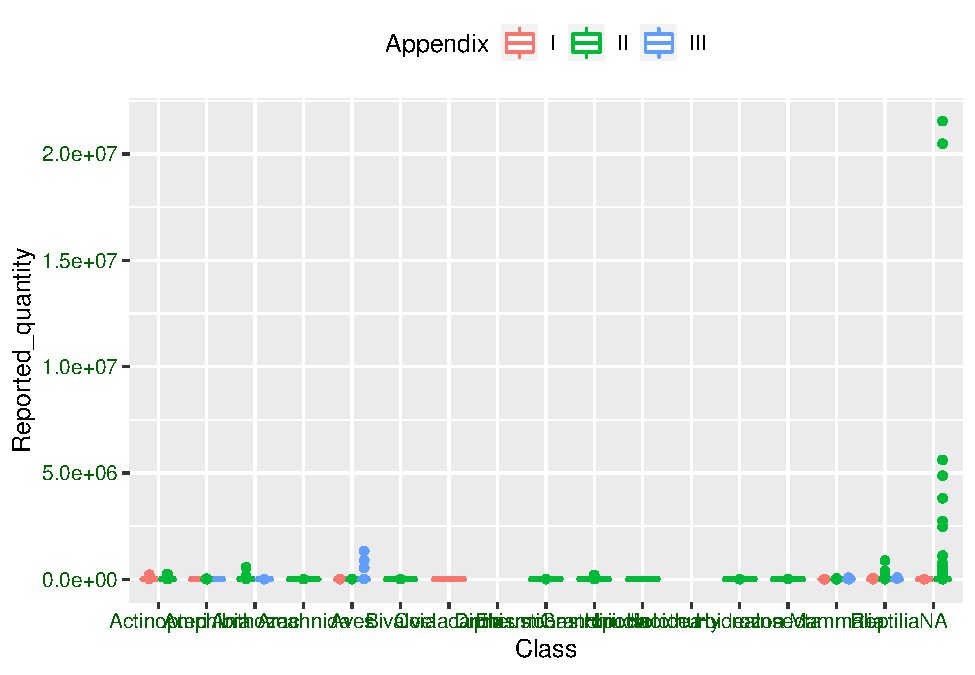
\includegraphics{Wood_ENV872_Project_files/figure-latex/unnamed-chunk-5-1.pdf}

\newpage

\hypertarget{dataset-information}{%
\section{Dataset Information}\label{dataset-information}}

\newpage

\hypertarget{exploratory-analysis}{%
\section{Exploratory Analysis}\label{exploratory-analysis}}

\newpage

\hypertarget{analysis}{%
\section{Analysis}\label{analysis}}

\hypertarget{question-1-insert-specific-question-here-and-add-additional-subsections-for-additional-questions-below-if-needed}{%
\subsection{Question 1: \textless insert specific question here and add
additional subsections for additional questions below, if
needed\textgreater{}}\label{question-1-insert-specific-question-here-and-add-additional-subsections-for-additional-questions-below-if-needed}}

\hypertarget{question-2}{%
\subsection{Question 2:}\label{question-2}}

\newpage

\hypertarget{summary-and-conclusions}{%
\section{Summary and Conclusions}\label{summary-and-conclusions}}

\newpage

\hypertarget{references}{%
\section{References}\label{references}}

\textless add references here if relevant, otherwise delete this
section\textgreater{}

\end{document}
